\chapter{Posterior Predictive Distributions}\label{app:postfitdists}

The $p_{\mu}$ and cos$\theta_{\mu}$ projections of the posterior predictions for each sample are shown in Figures \ref{fig:priorpost_fhc_papp}--\ref{fig:priorpost_rhc_numu_tapp}, along with the prior predictions and data.

\begin{figure}[!htbp]
\centering
\begin{subfigure}{.24\textwidth}
  \centering
  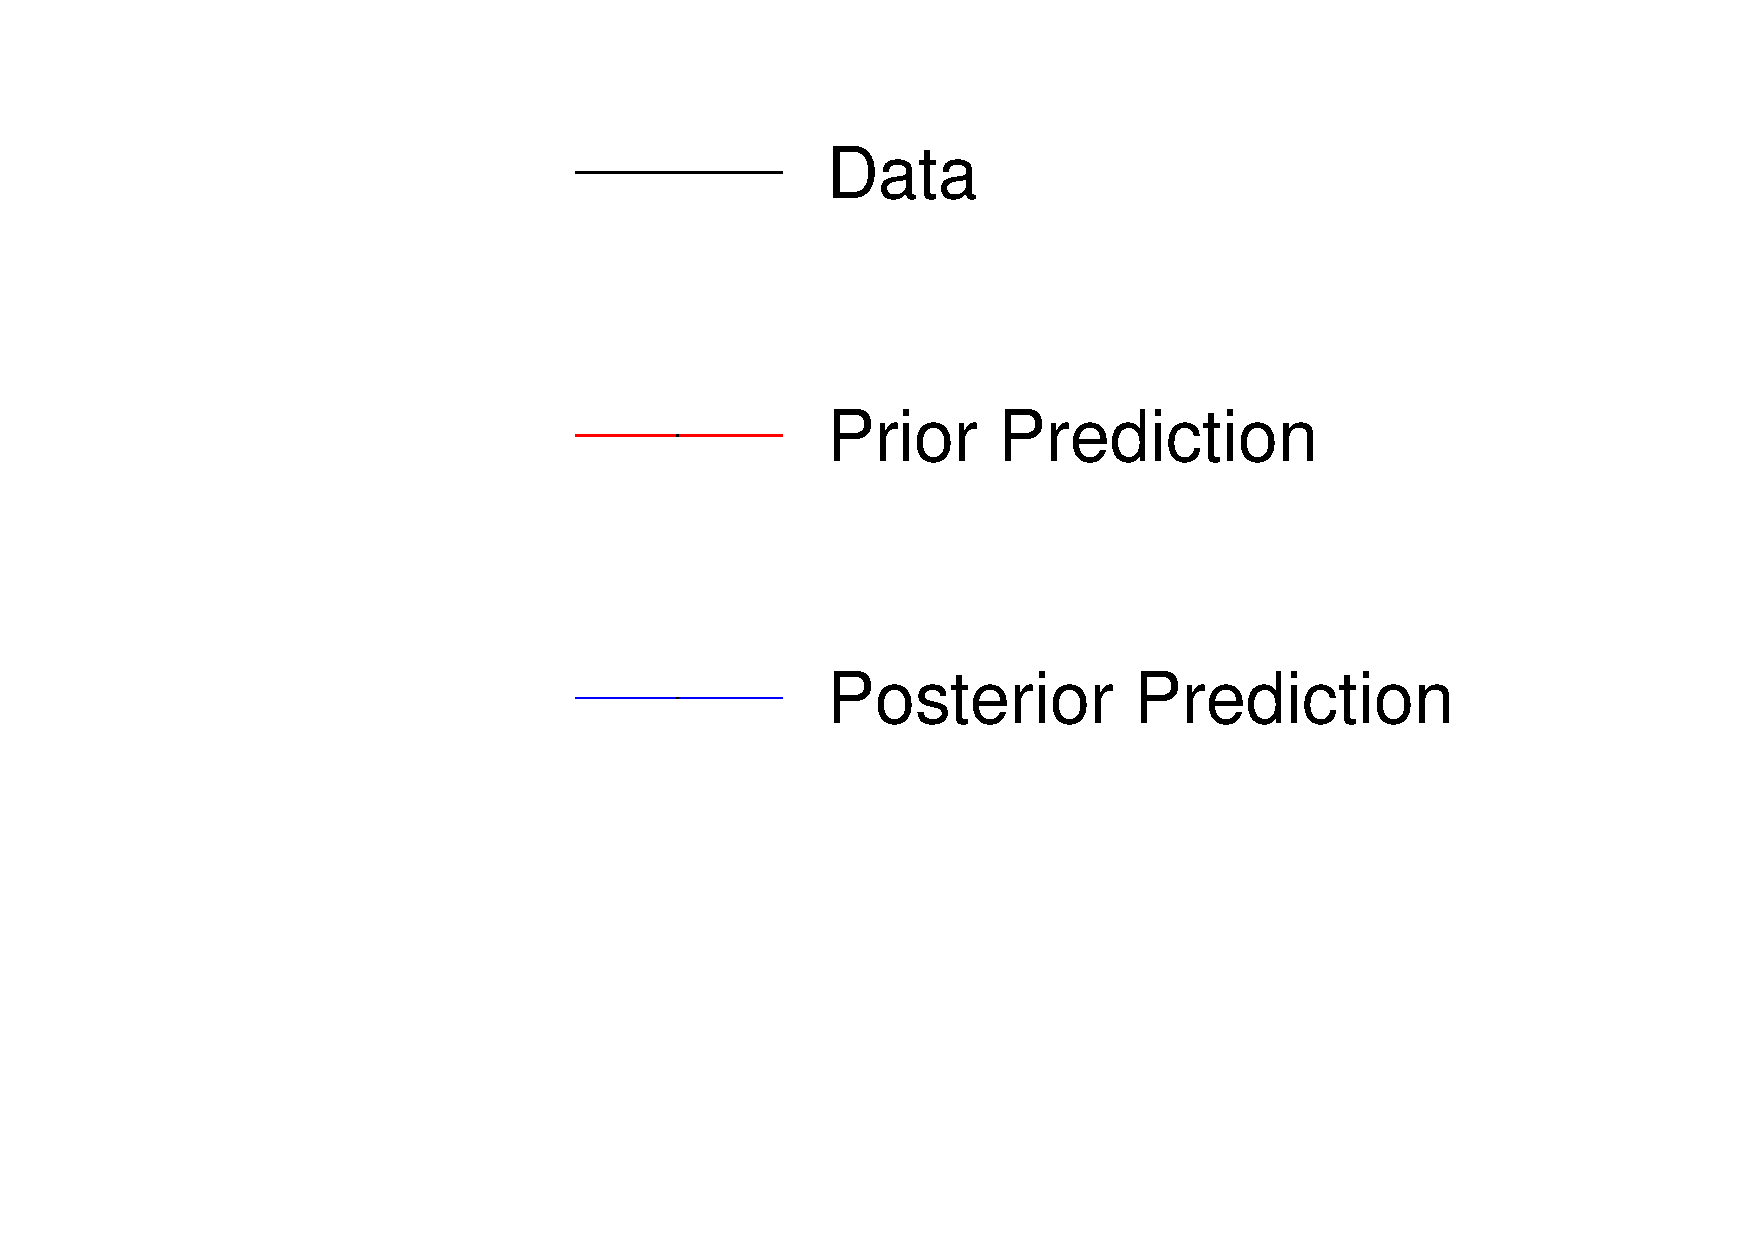
\includegraphics[width=\linewidth, clip]{figs/prior1dleg.pdf}
\end{subfigure}

\begin{subfigure}{0.49\textwidth}
  \centering
  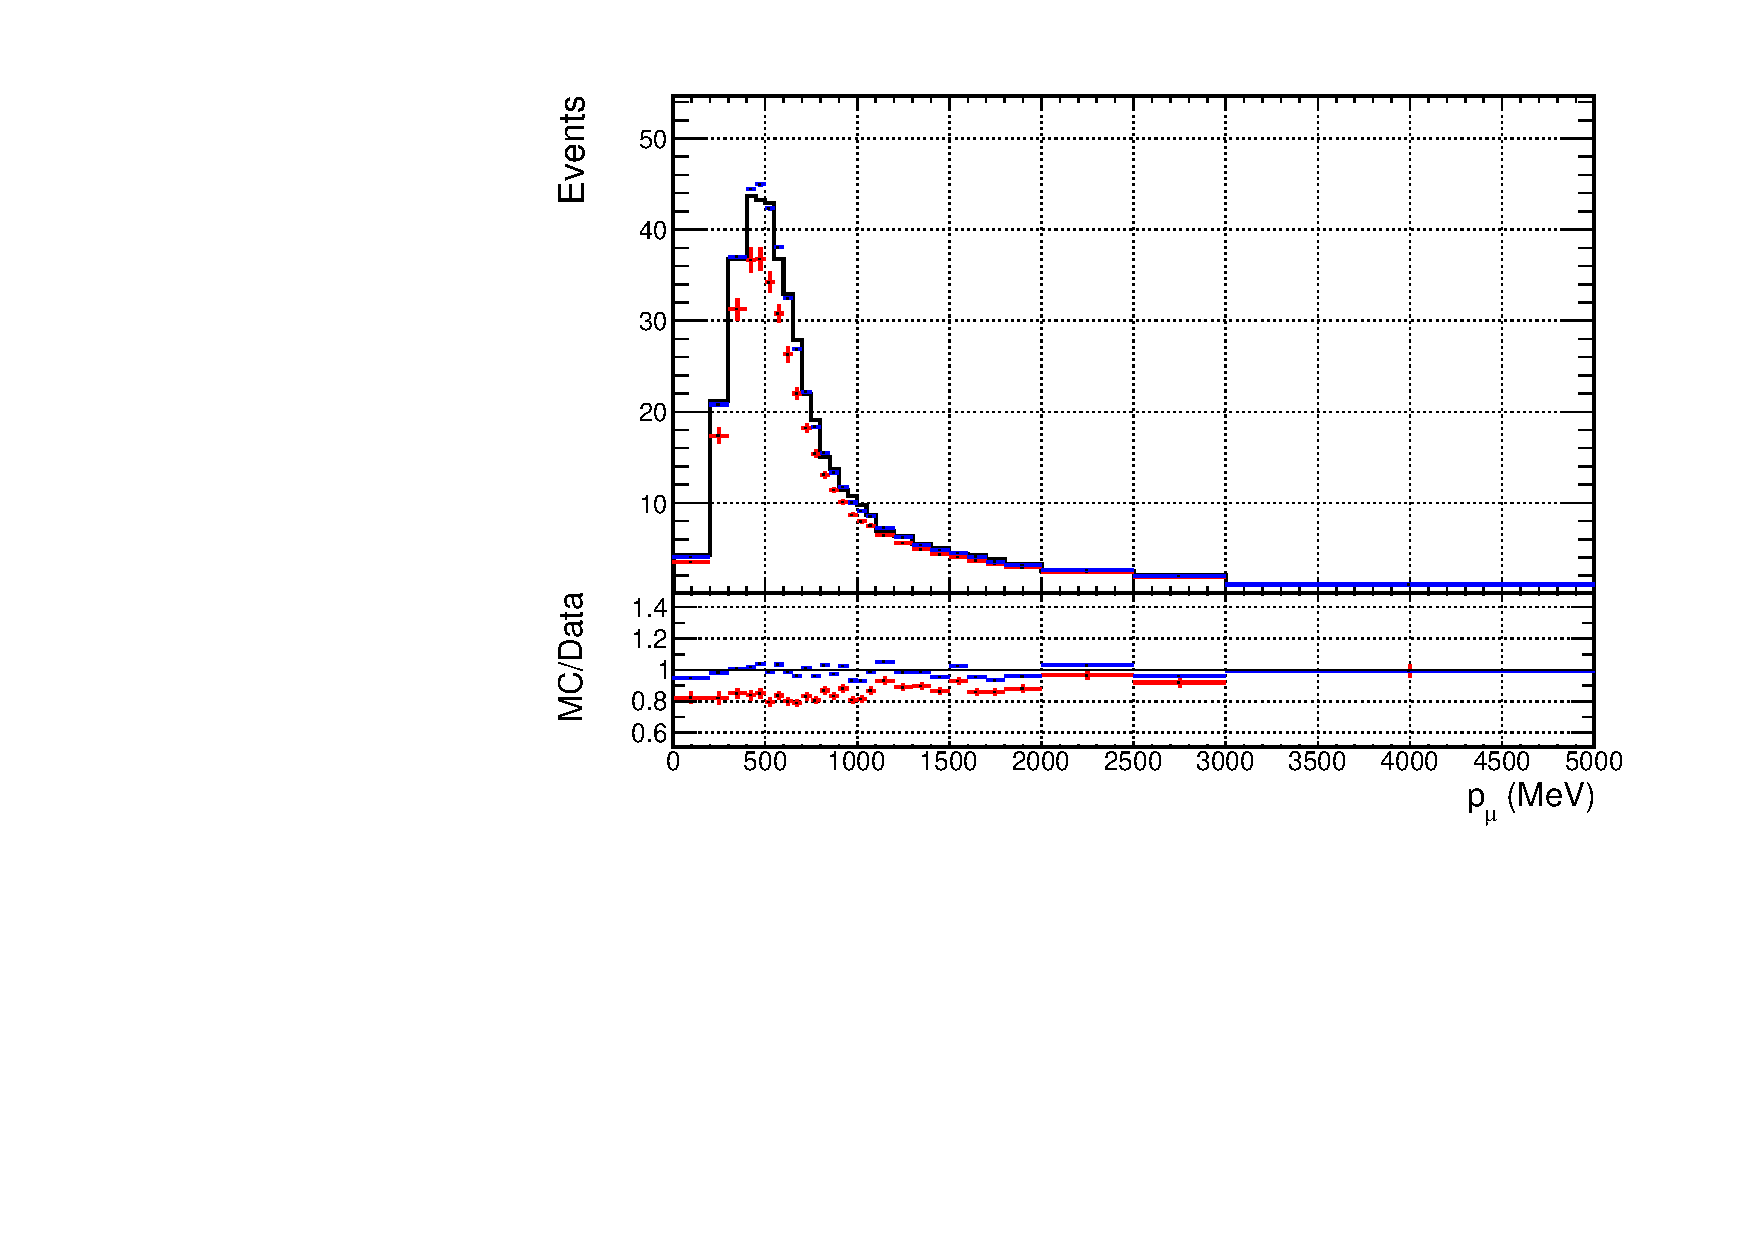
\includegraphics[width=\textwidth]{figs/priorpred1D_p_FGD1_numuCC_0pi}
  \caption{FGD1 FHC $\nu_{\mu}$ 0$\pi$}
\end{subfigure}
\begin{subfigure}{0.49\textwidth}
  \centering
  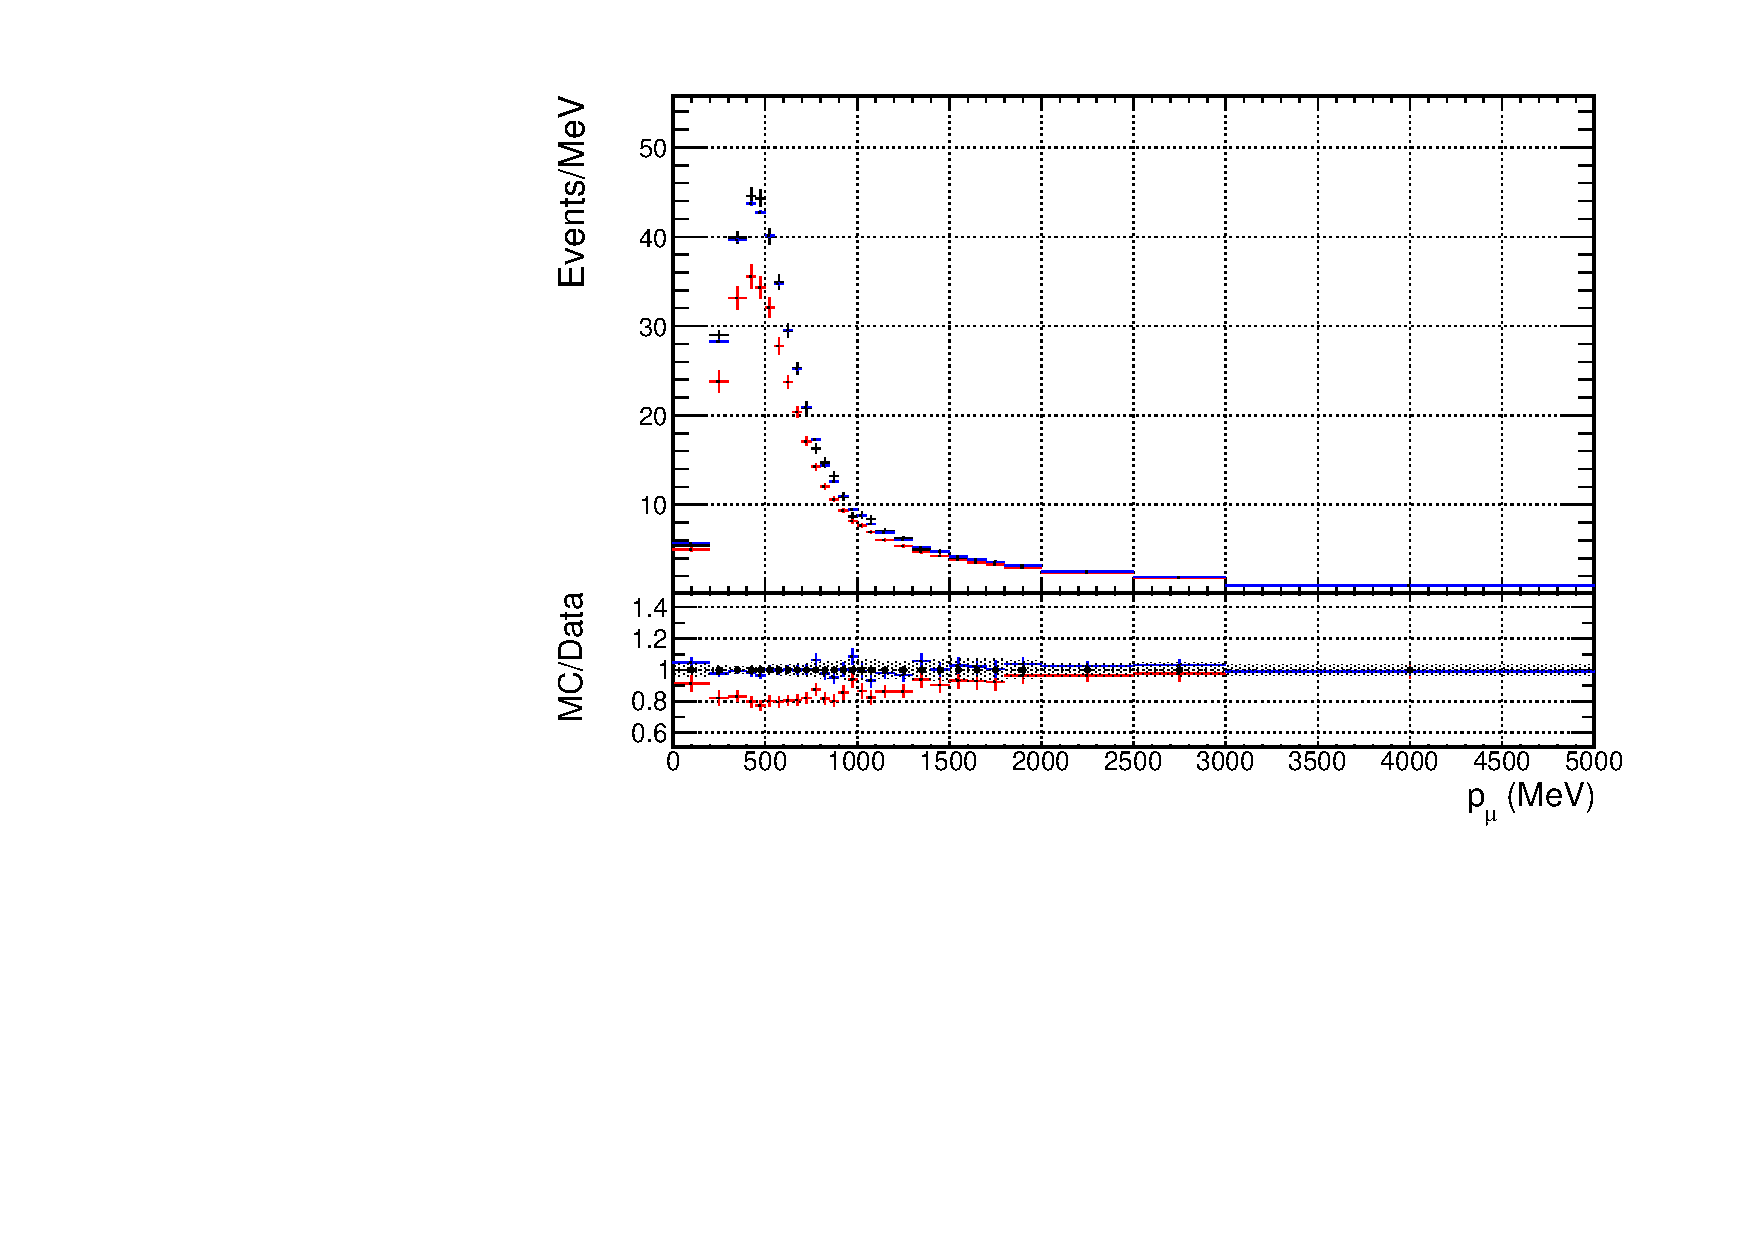
\includegraphics[width=\textwidth]{figs/priorpred1D_p_FGD2_numuCC_0pi}
  \caption{FGD2 FHC $\nu_{\mu}$ 0$\pi$}
\end{subfigure}

\begin{subfigure}{0.49\textwidth}
  \centering
  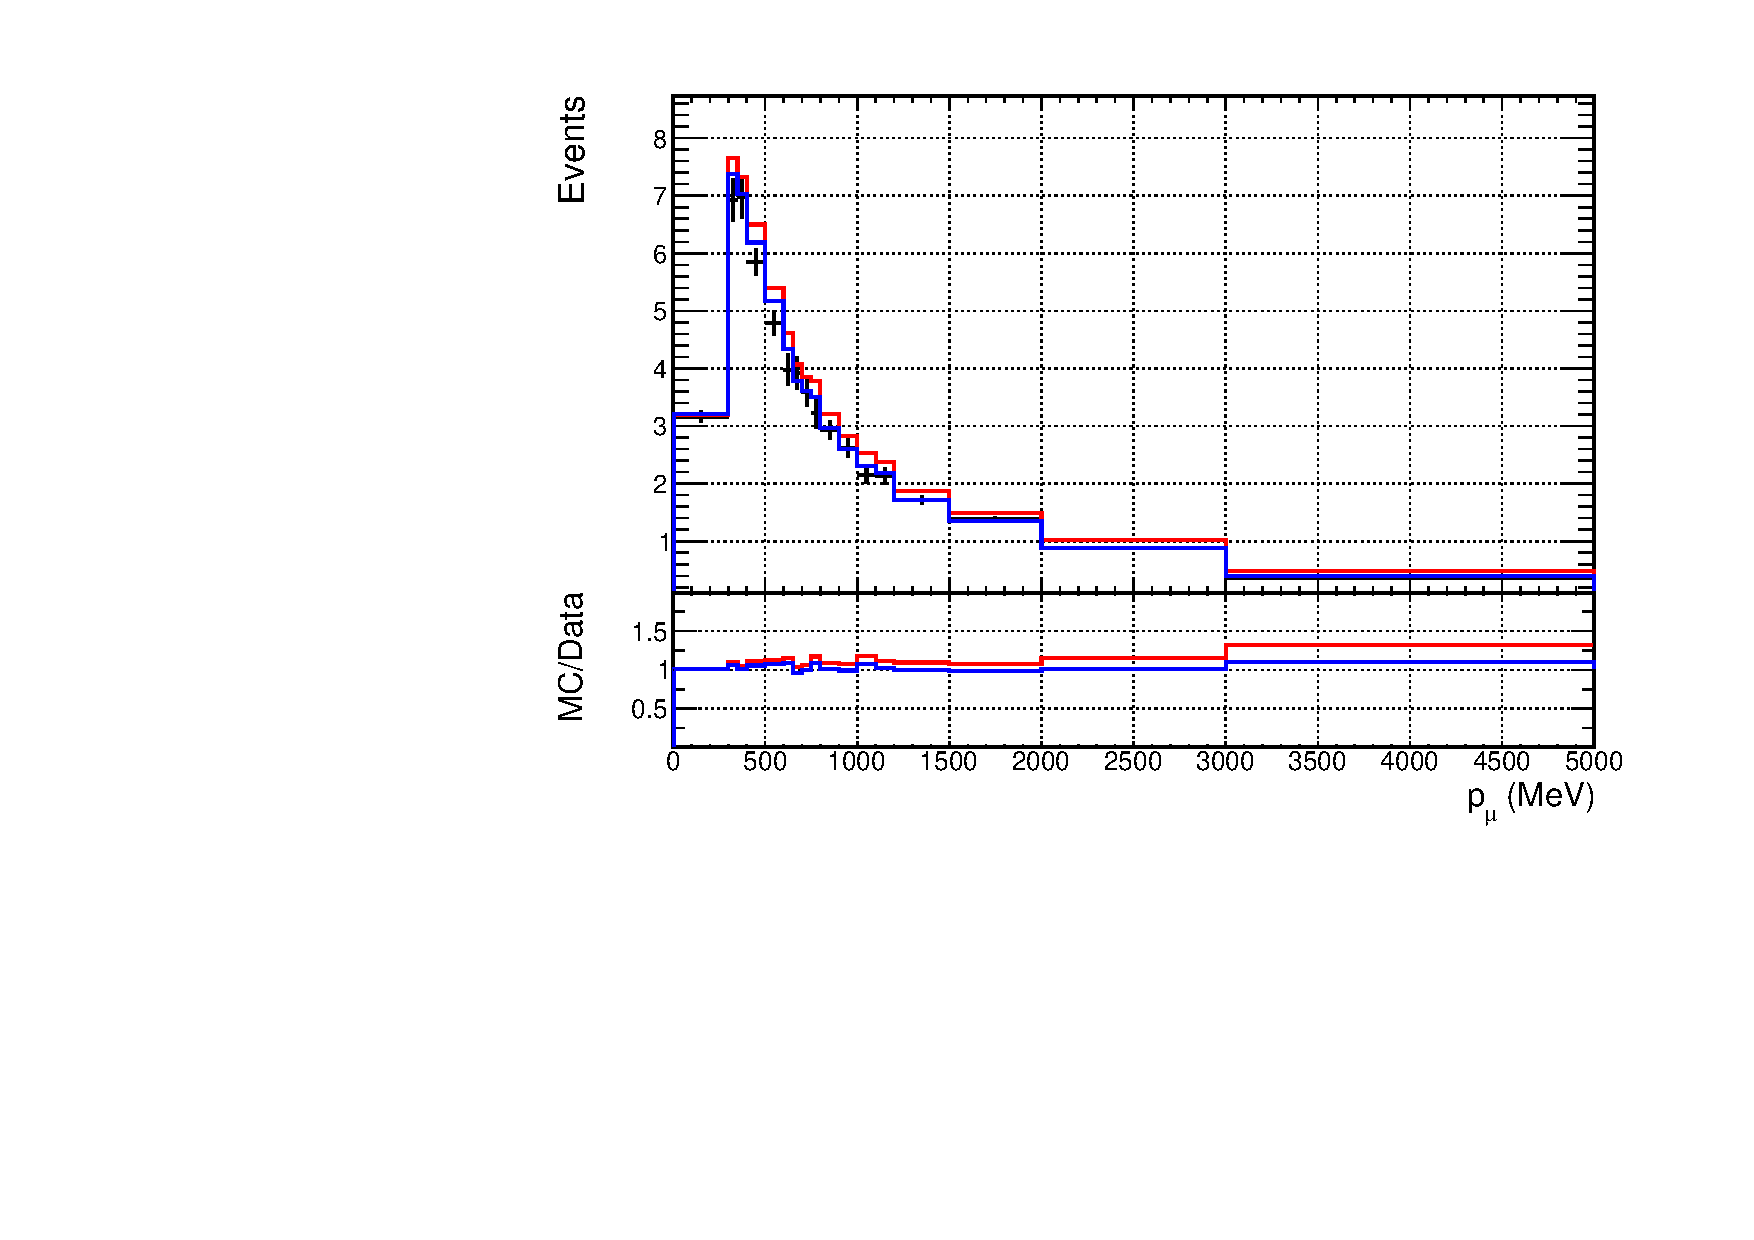
\includegraphics[width=\textwidth]{figs/priorpred1D_p_FGD1_numuCC_1pi}
  \caption{FGD1 FHC $\nu_{\mu}$ 1$\pi$}
\end{subfigure}
\begin{subfigure}{0.49\textwidth}
  \centering
  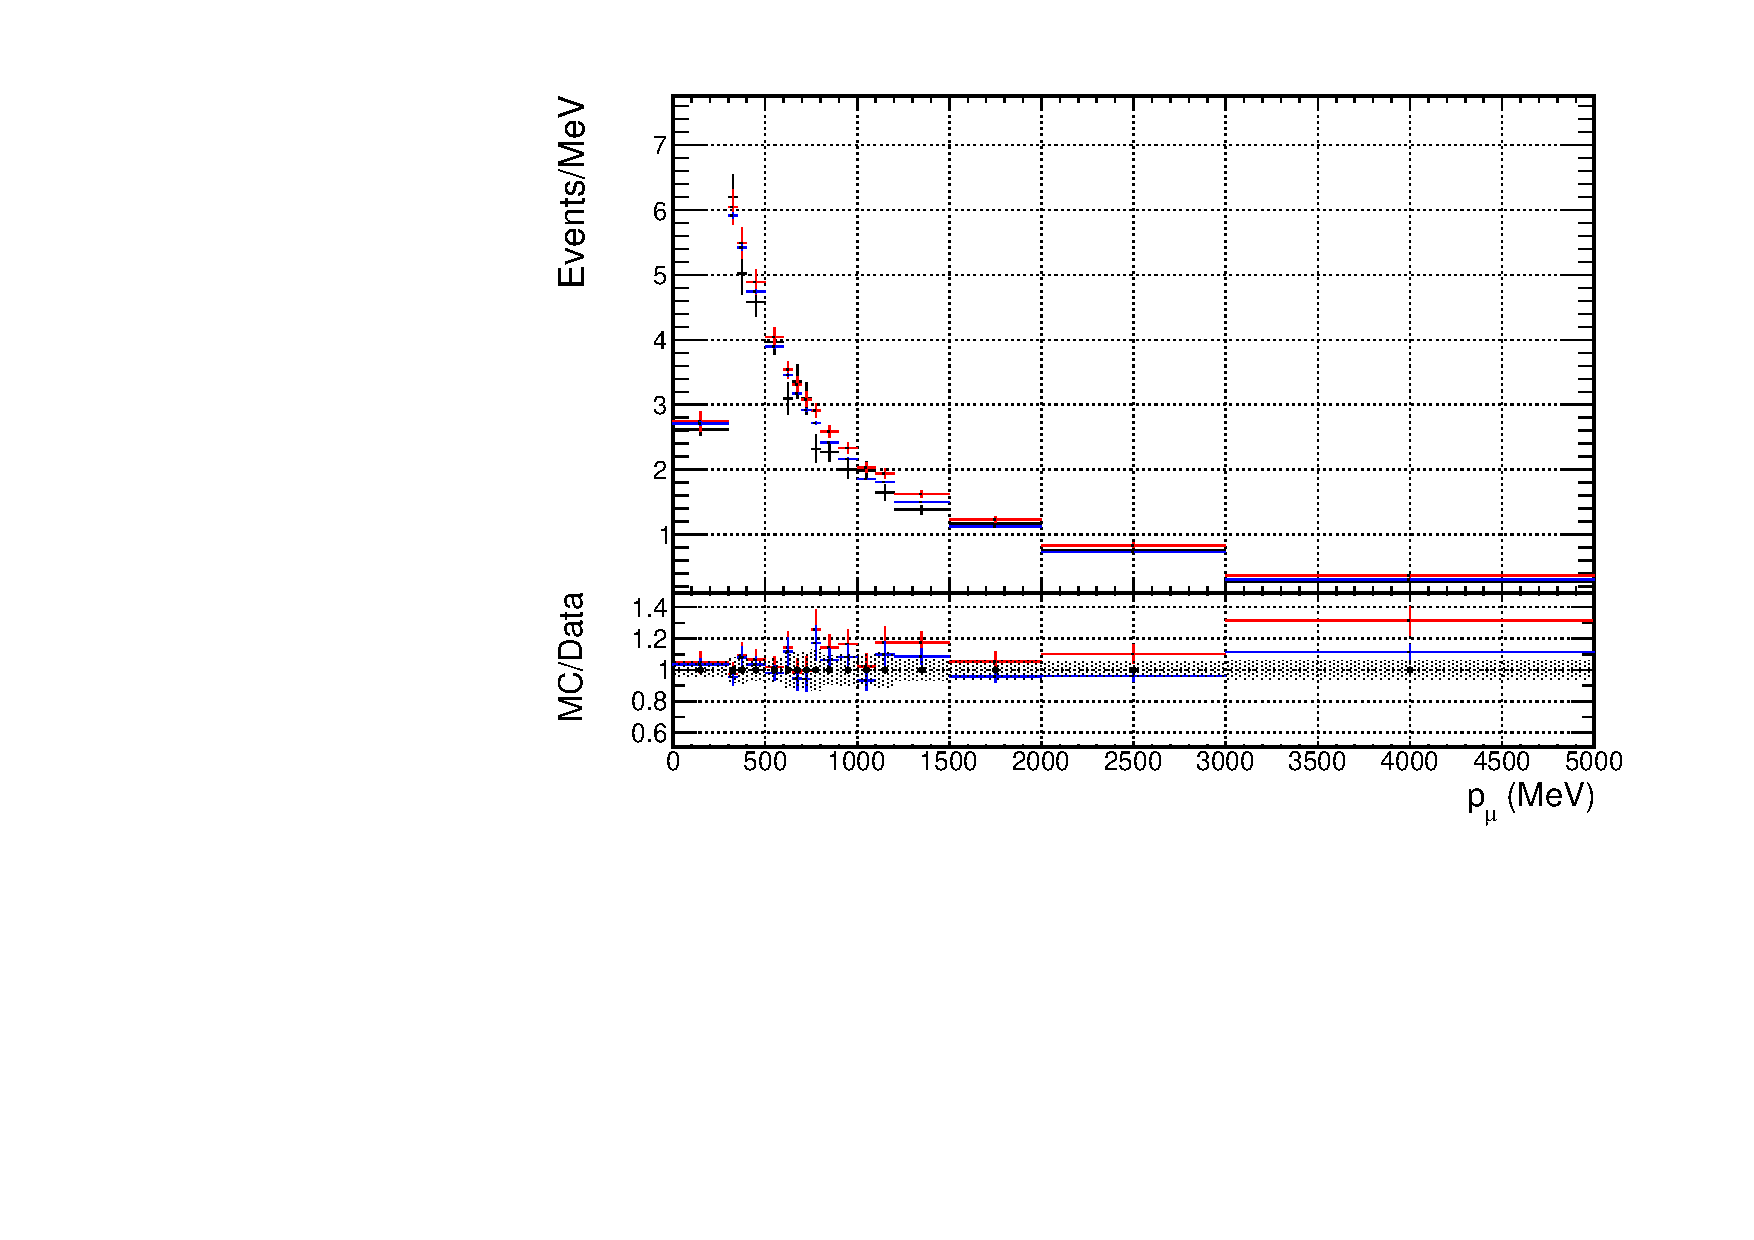
\includegraphics[width=\textwidth]{figs/priorpred1D_p_FGD2_numuCC_1pi}
  \caption{FGD2 FHC $\nu_{\mu}$ 1$\pi$}
\end{subfigure}

\begin{subfigure}{0.49\textwidth}
  \centering
  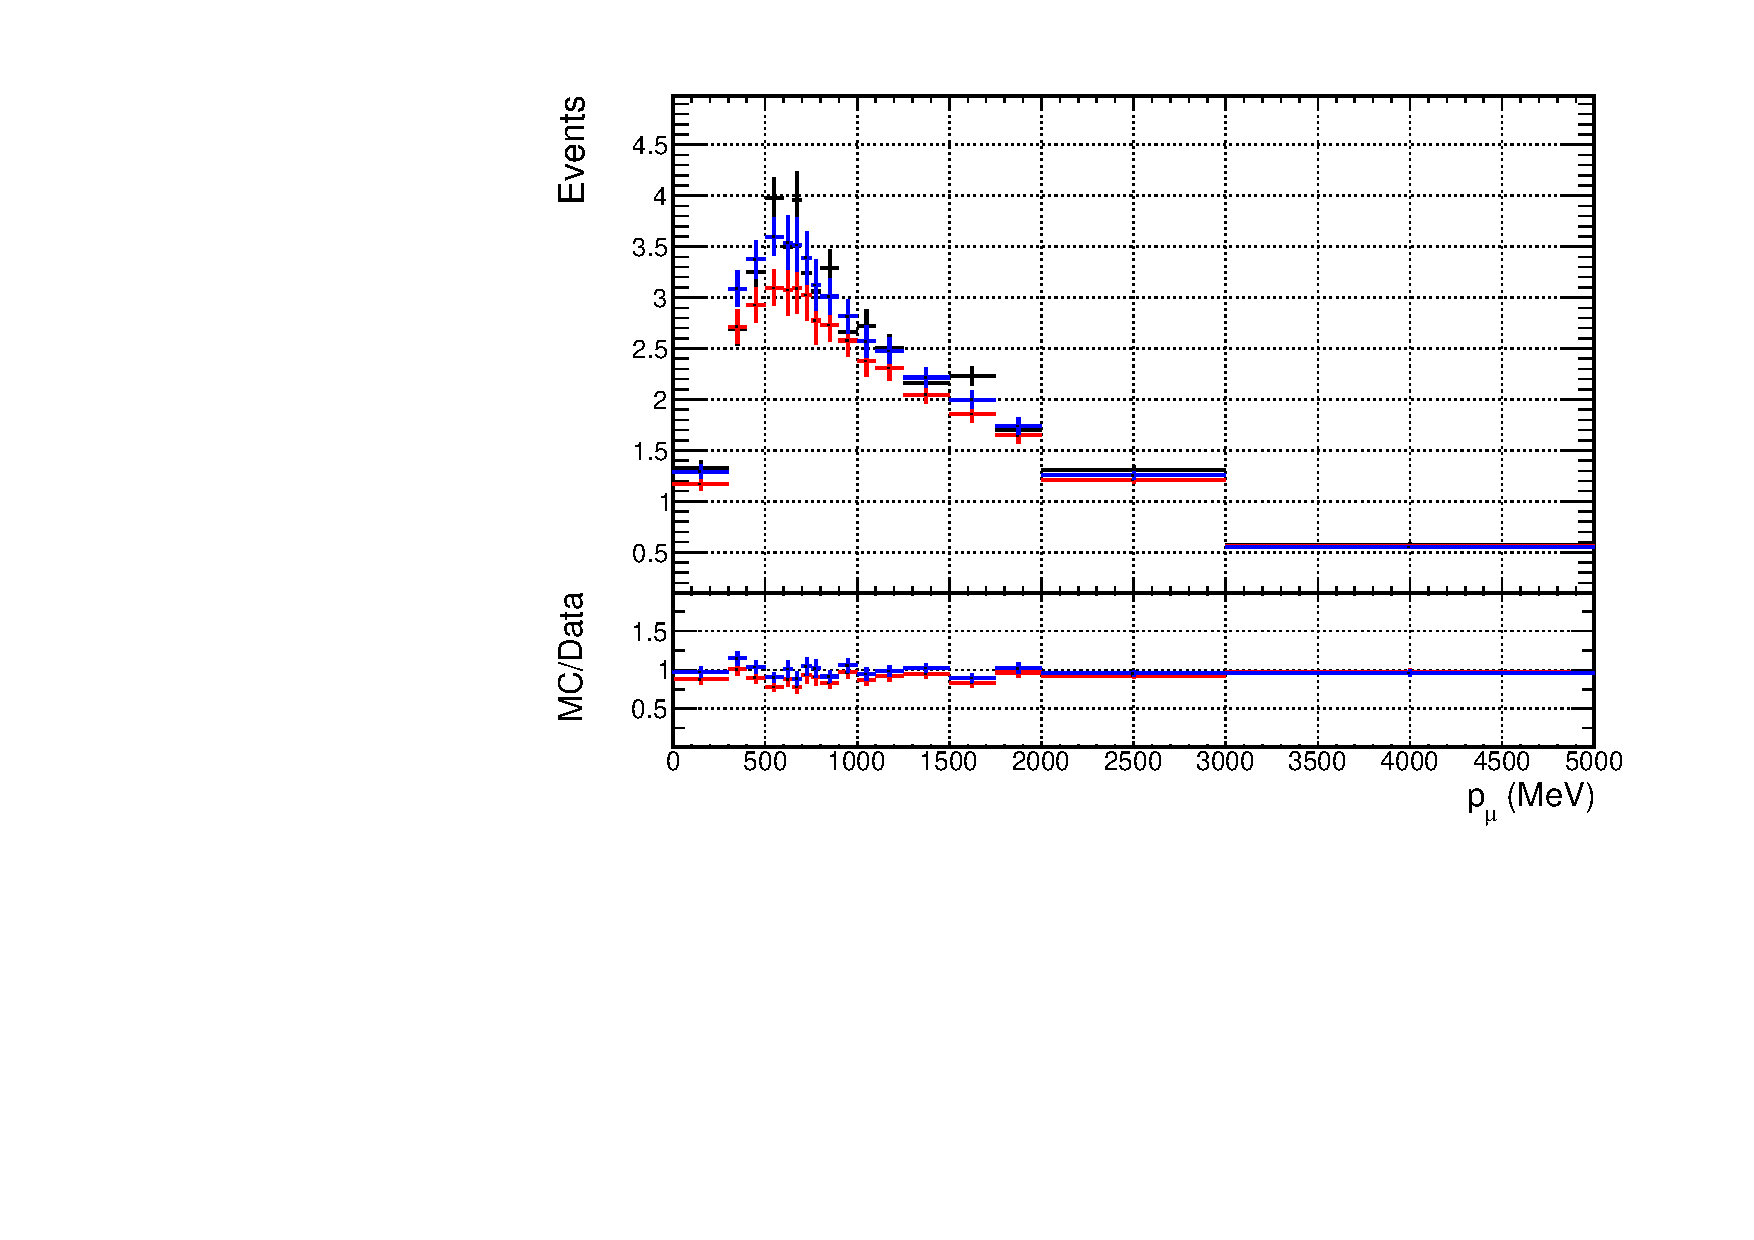
\includegraphics[width=\textwidth]{figs/priorpred1D_p_FGD1_numuCC_other}
  \caption{FGD1 FHC $\nu_{\mu}$ Other}
\end{subfigure}
\begin{subfigure}{0.49\textwidth}
  \centering
  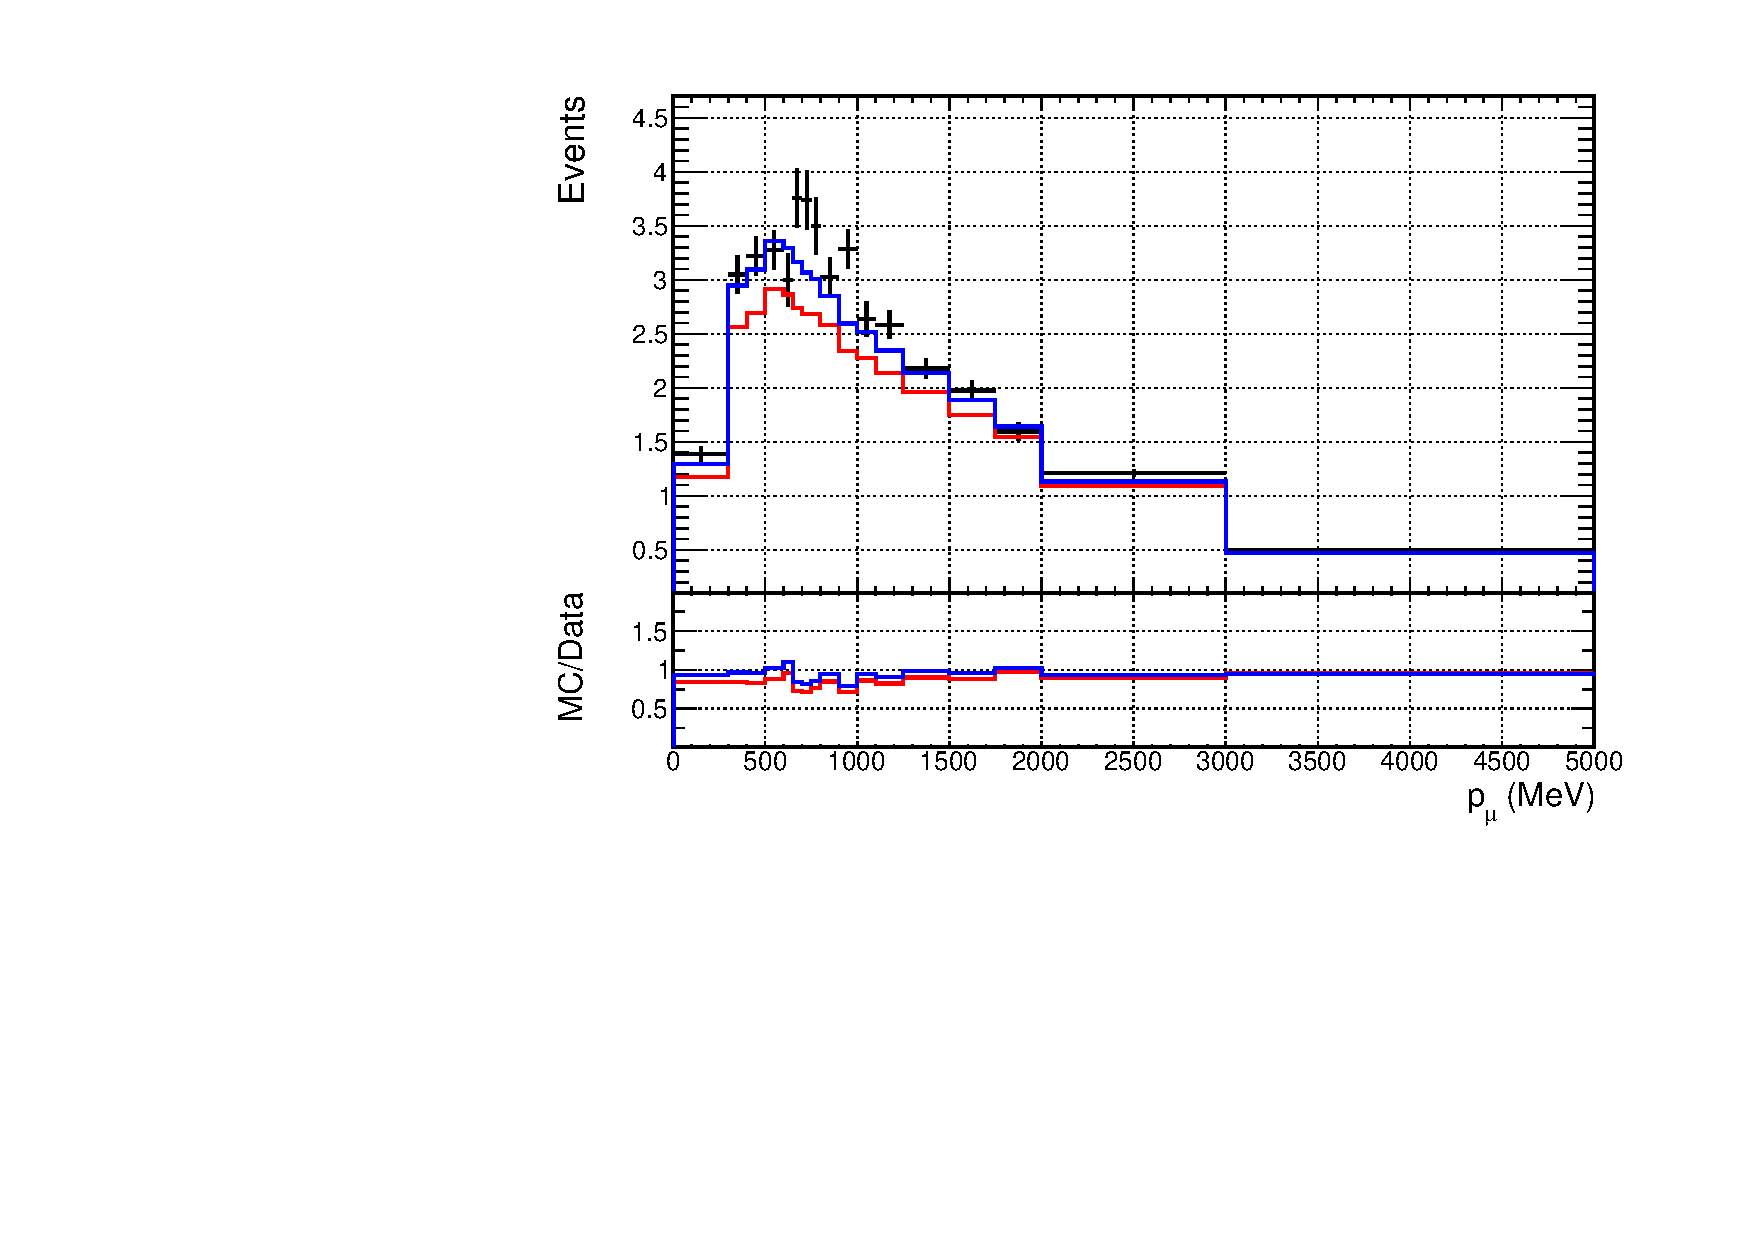
\includegraphics[width=\textwidth]{figs/priorpred1D_p_FGD2_numuCC_other}
  \caption{FGD2 FHC $\nu_{\mu}$ Other}
\end{subfigure}
\caption{$p_{\mu}$ projections of the prior and posterior predictive distributions and data for FHC \numu selections.}
\label{fig:priorpost_fhc_papp}
\end{figure}

\begin{figure}[!htbp]
\centering
\begin{subfigure}{.24\textwidth}
  \centering
  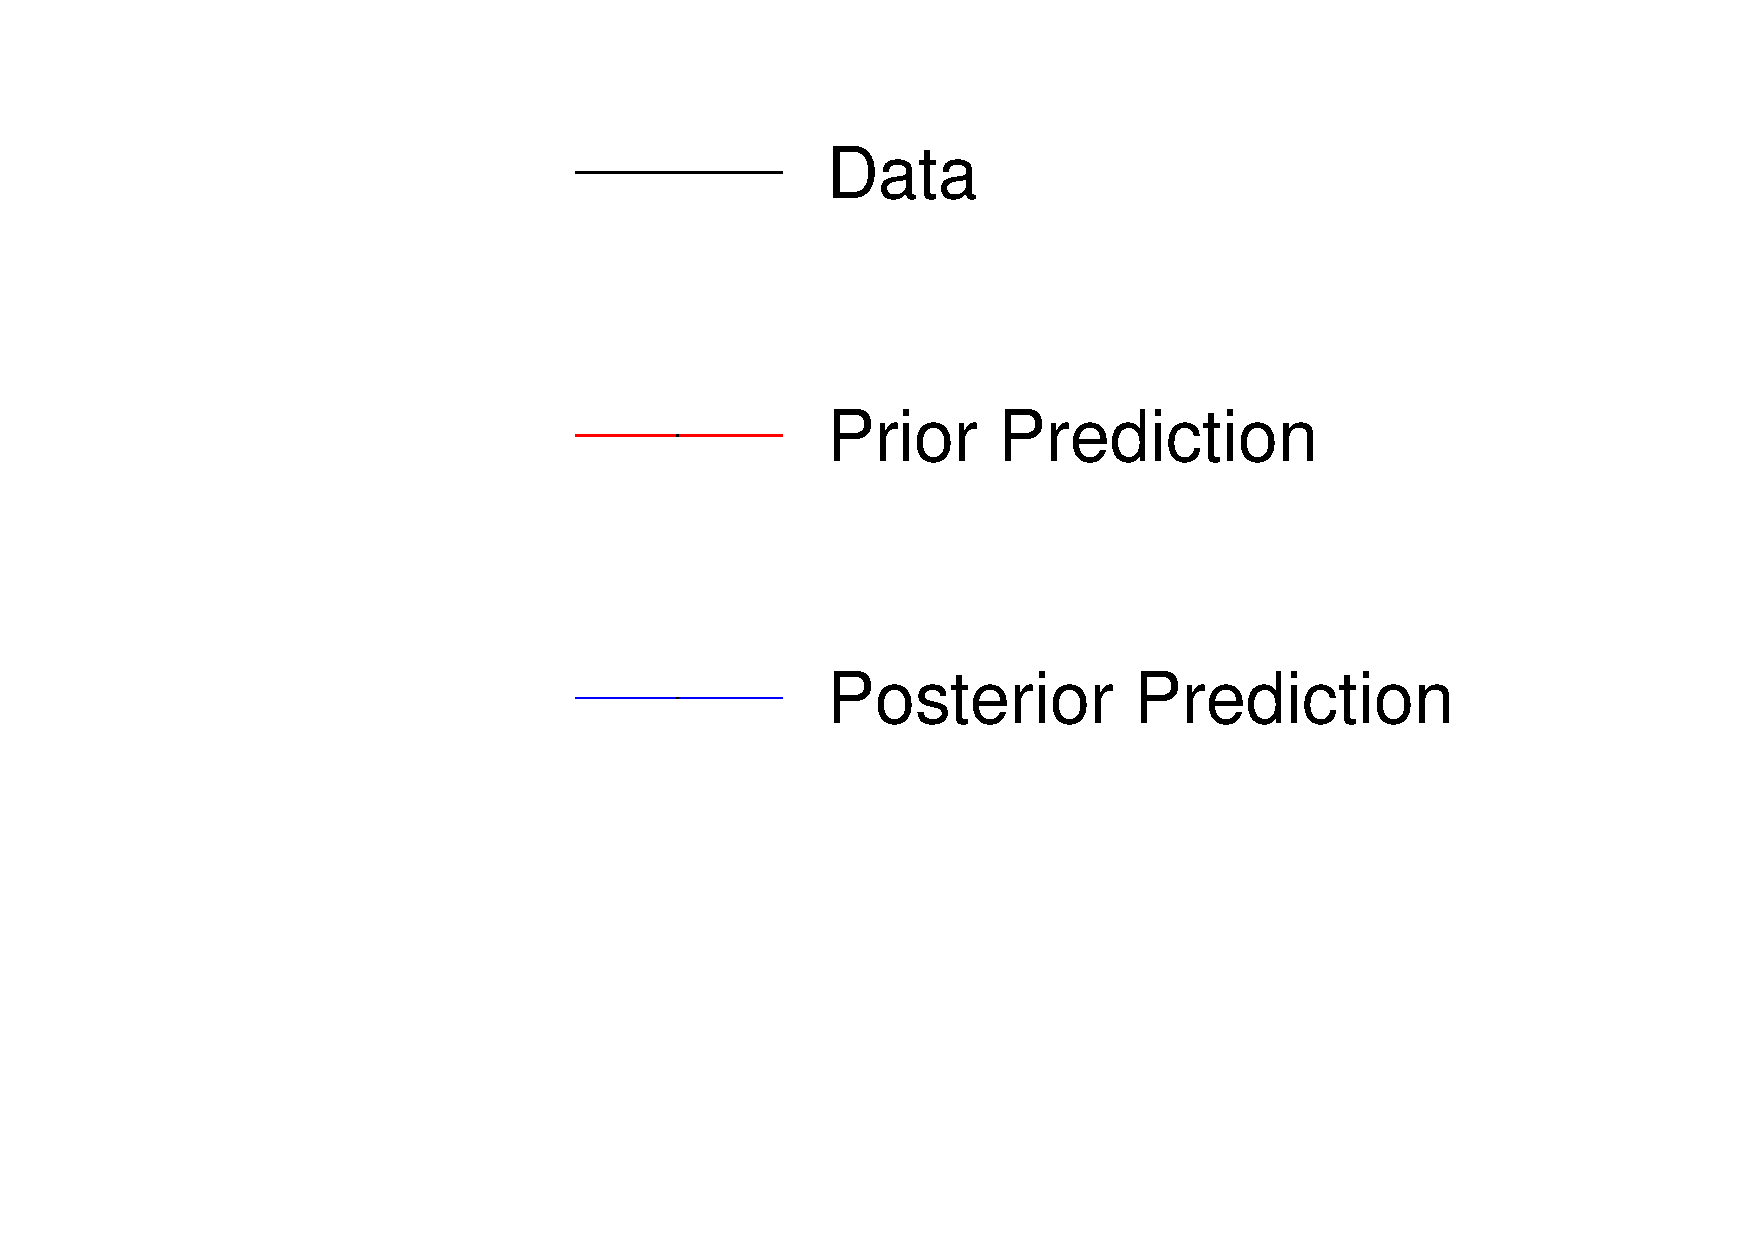
\includegraphics[width=\linewidth, clip]{figs/prior1dleg.pdf}
\end{subfigure}

\begin{subfigure}{0.49\textwidth}
  \centering
  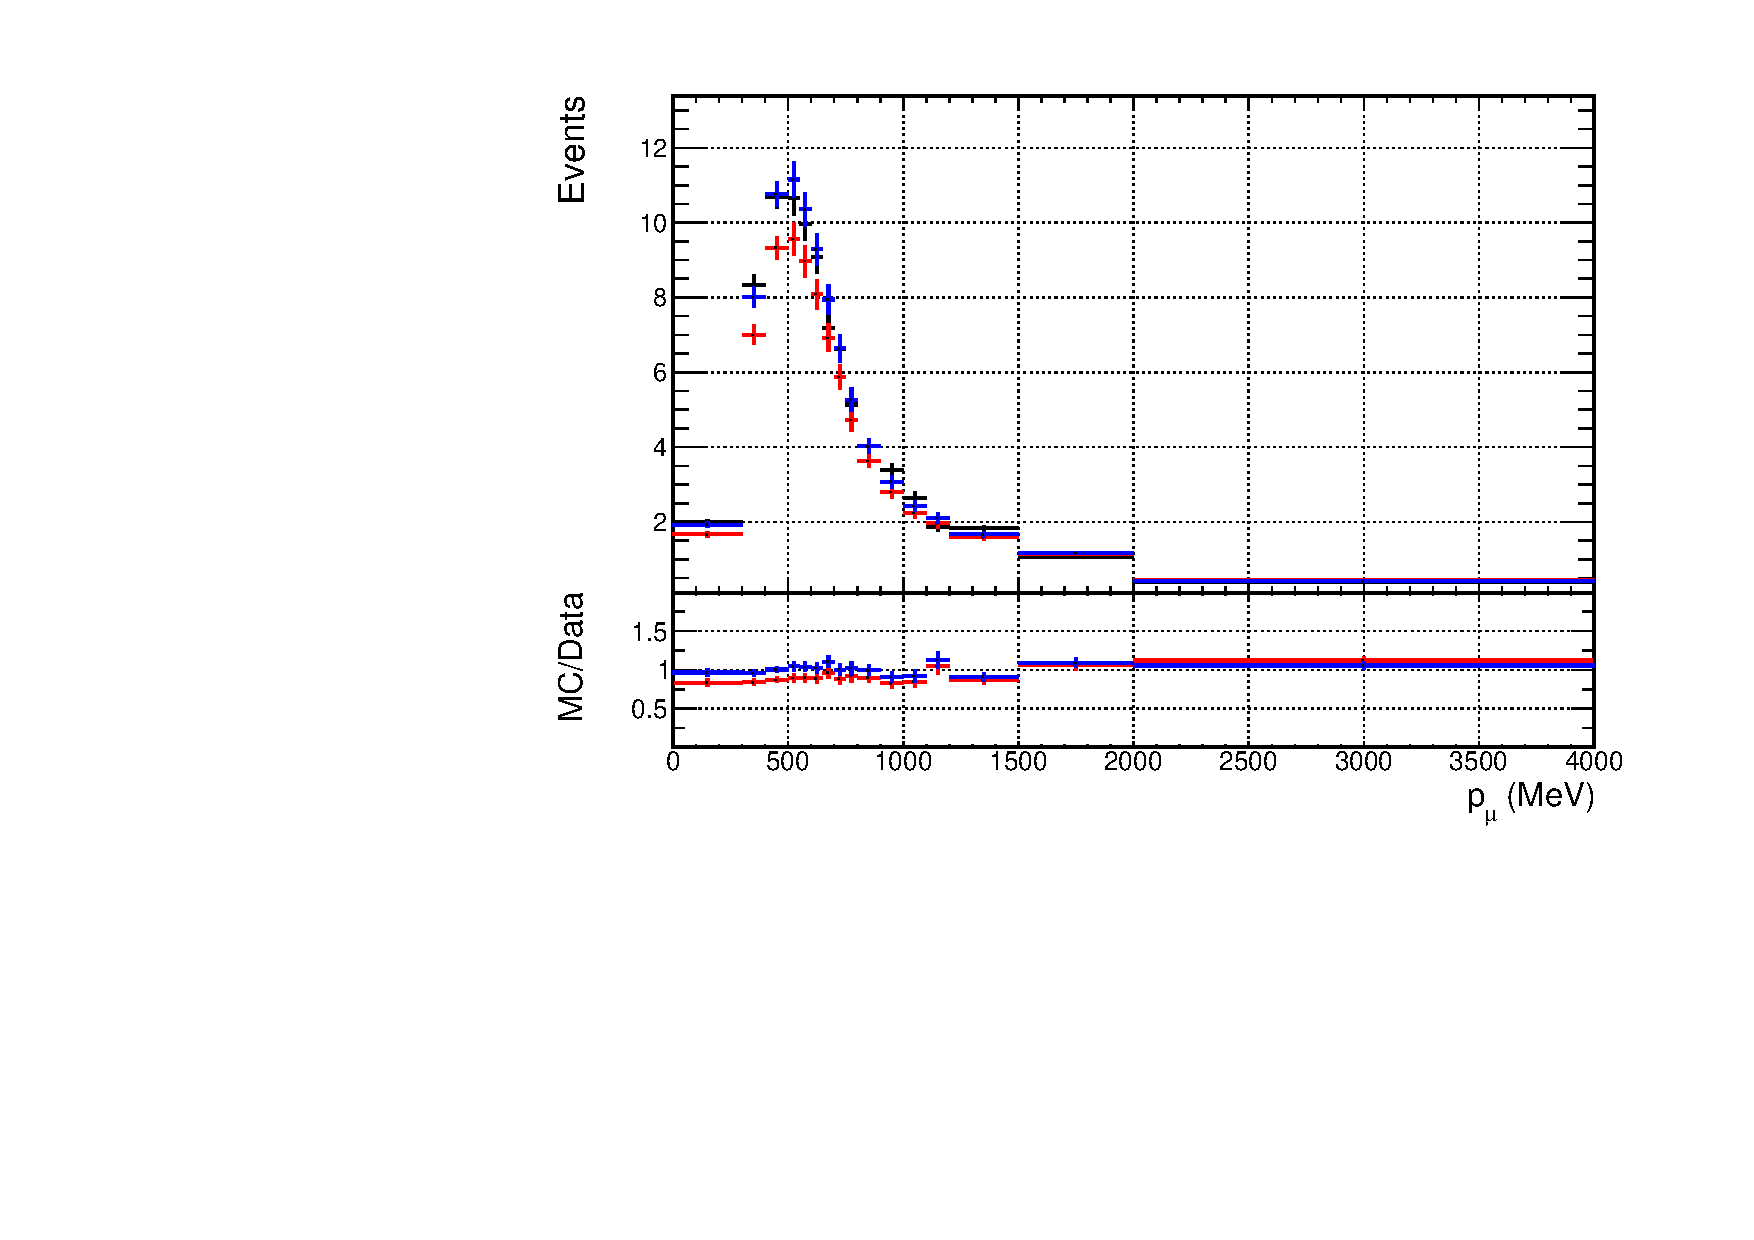
\includegraphics[width=\textwidth]{figs/priorpred1D_p_FGD1_anti-numuCC_0pi}
  \caption{FGD1 RHC $\bar{\nu_{\mu}}$ 0$\pi$}
\end{subfigure}
\begin{subfigure}{0.49\textwidth}
  \centering
  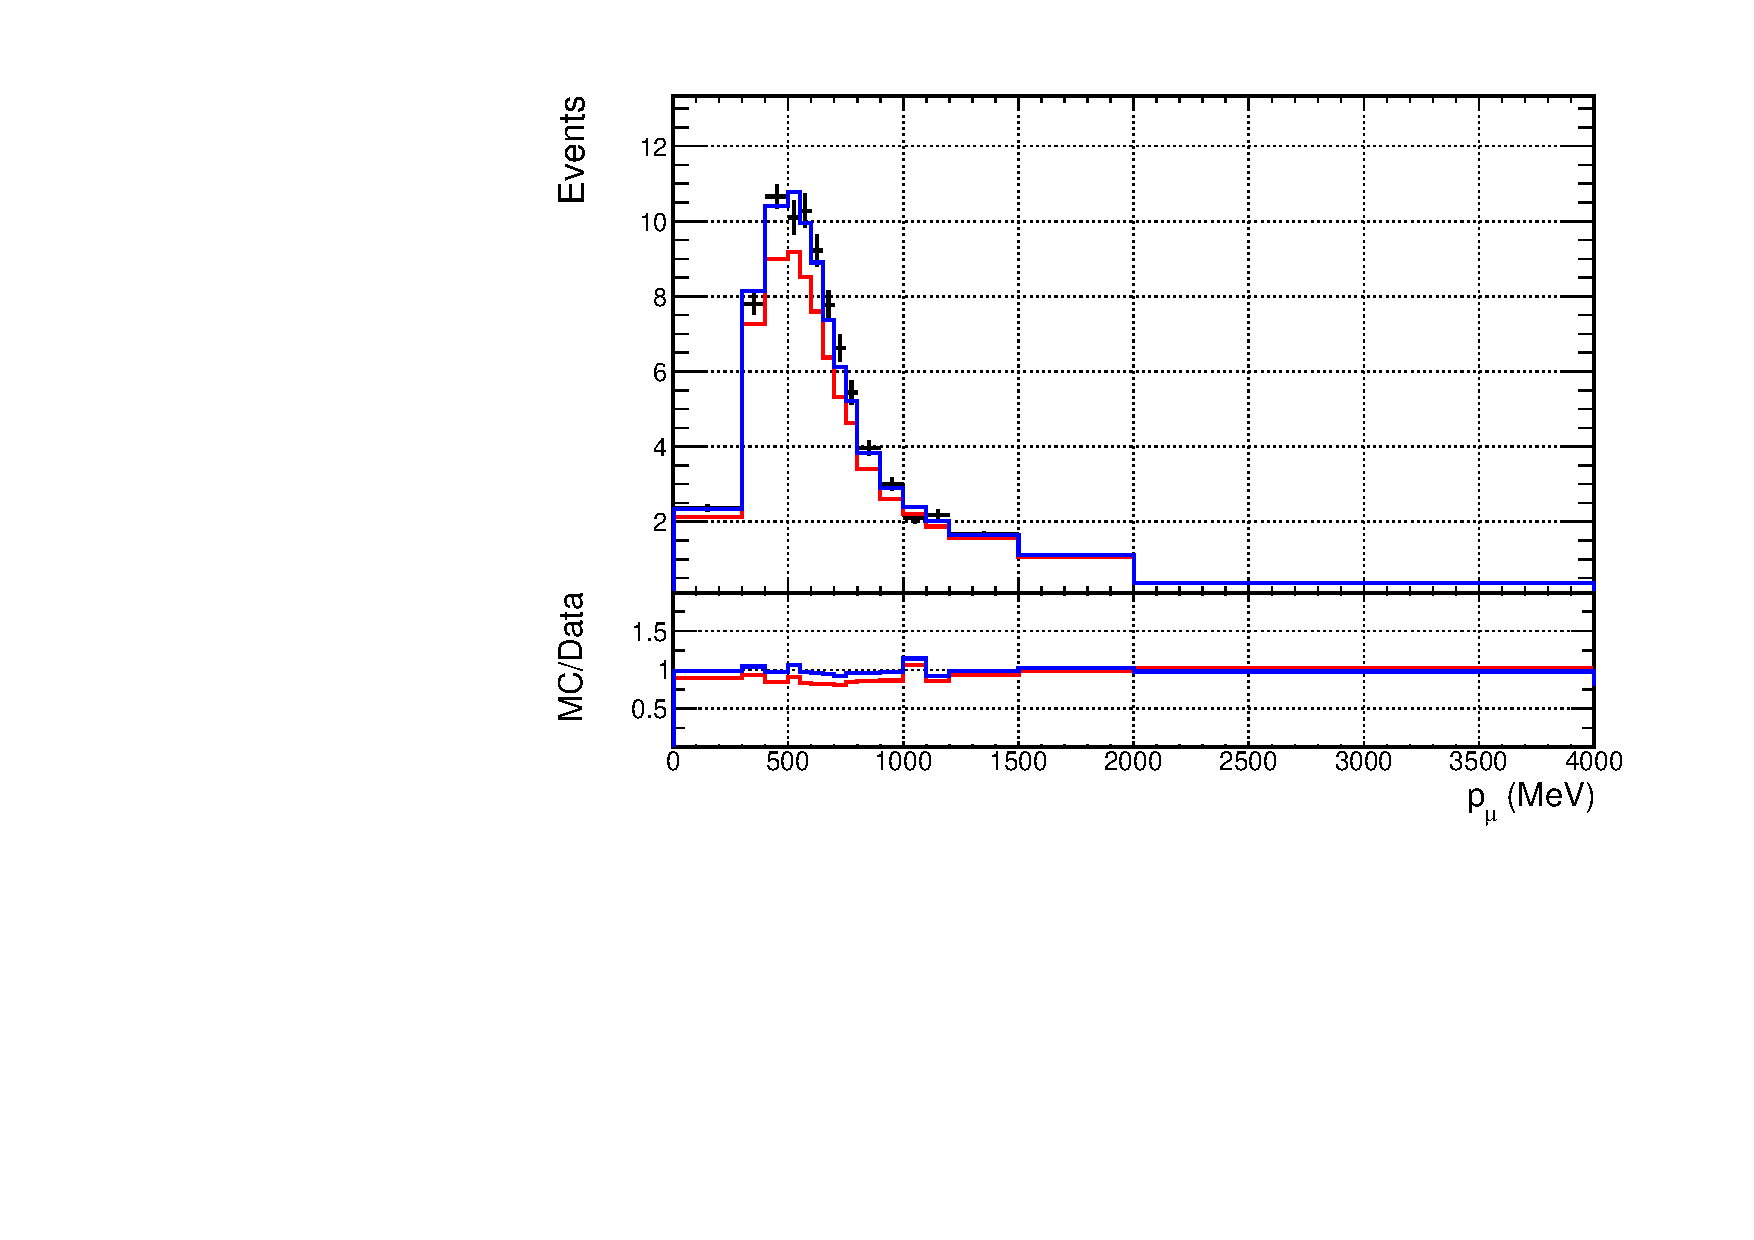
\includegraphics[width=\textwidth]{figs/priorpred1D_p_FGD2_anti-numuCC_0pi}
  \caption{FGD2 RHC $\bar{\nu_{\mu}}$ 0$\pi$}
\end{subfigure}

\begin{subfigure}{0.49\textwidth}
  \centering
  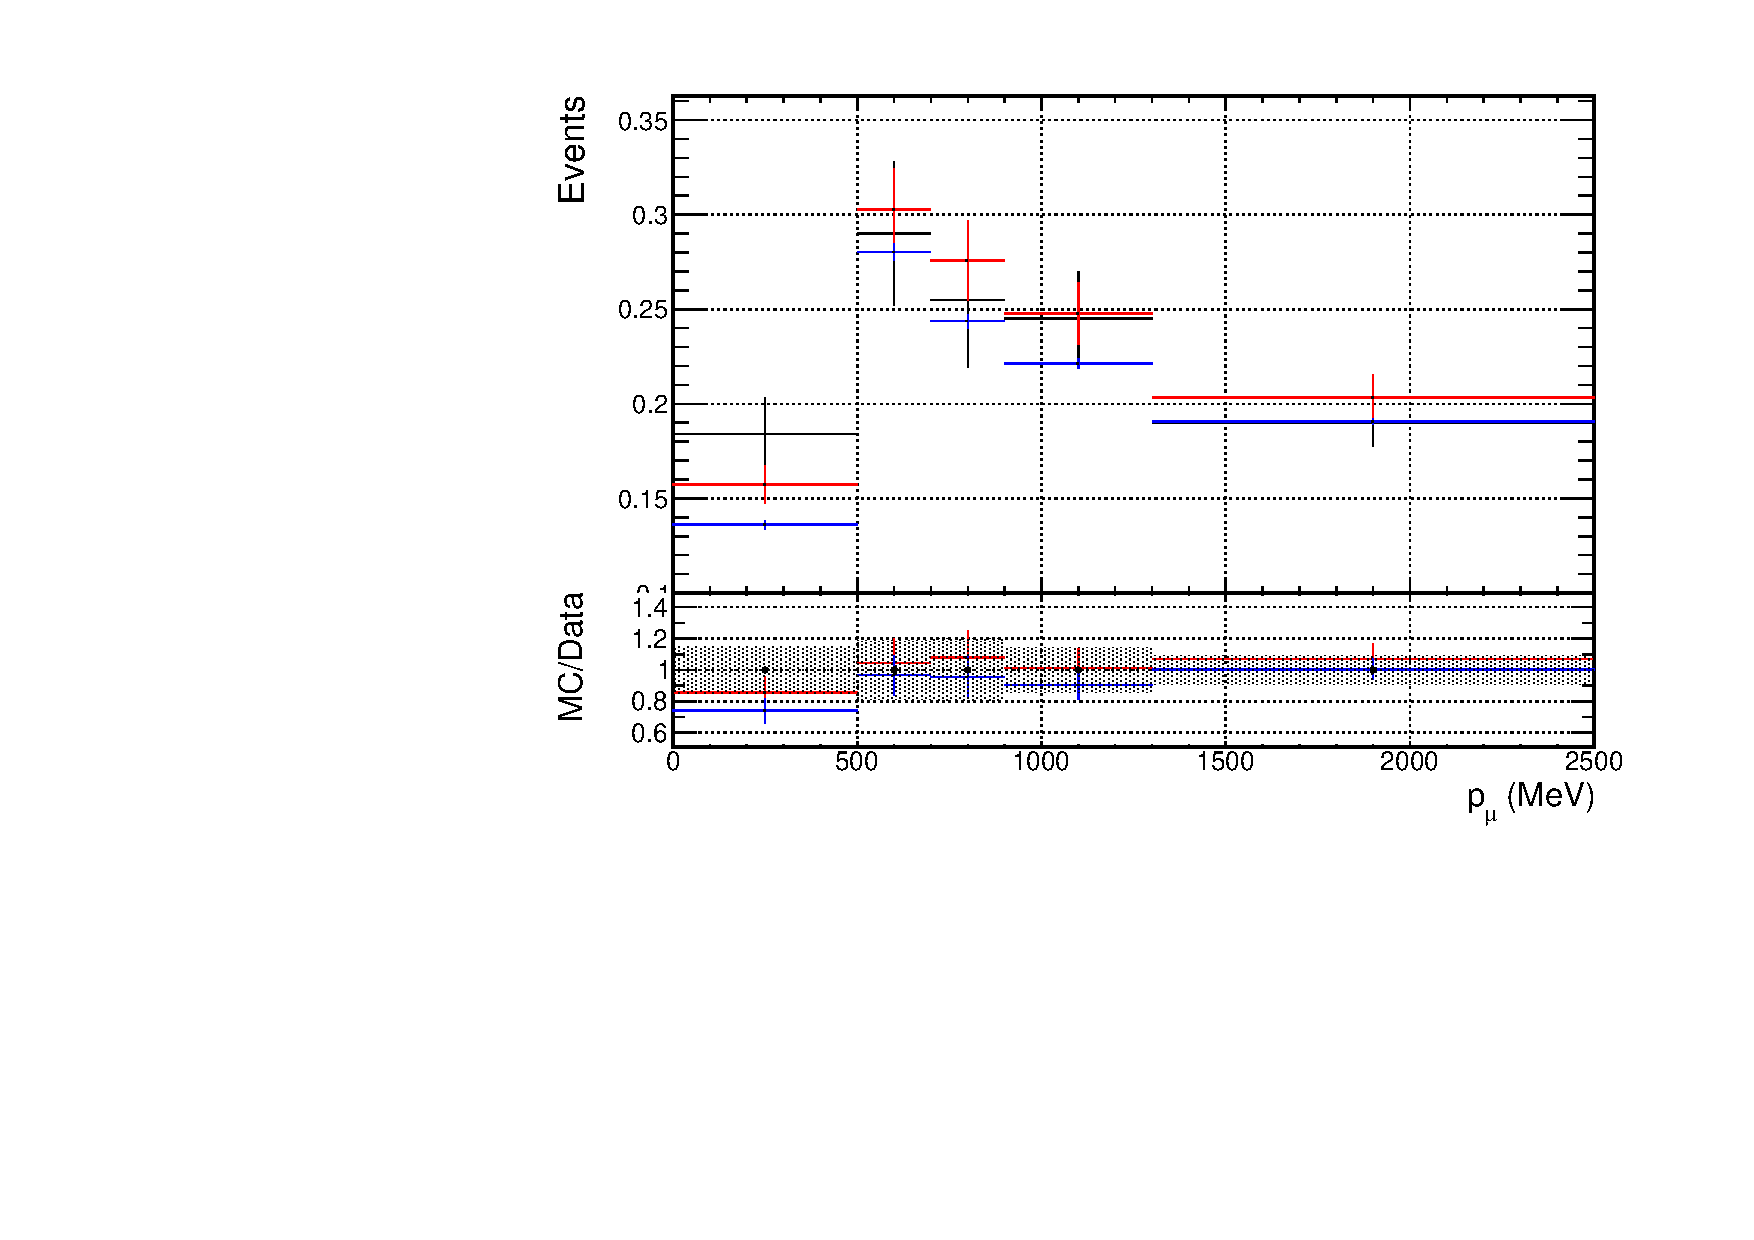
\includegraphics[width=\textwidth]{figs/priorpred1D_p_FGD1_anti-numuCC_1pi}
  \caption{FGD1 RHC $\bar{\nu_{\mu}}$ 1$\pi$}
\end{subfigure}
\centering
\begin{subfigure}{0.49\textwidth}
  \centering
  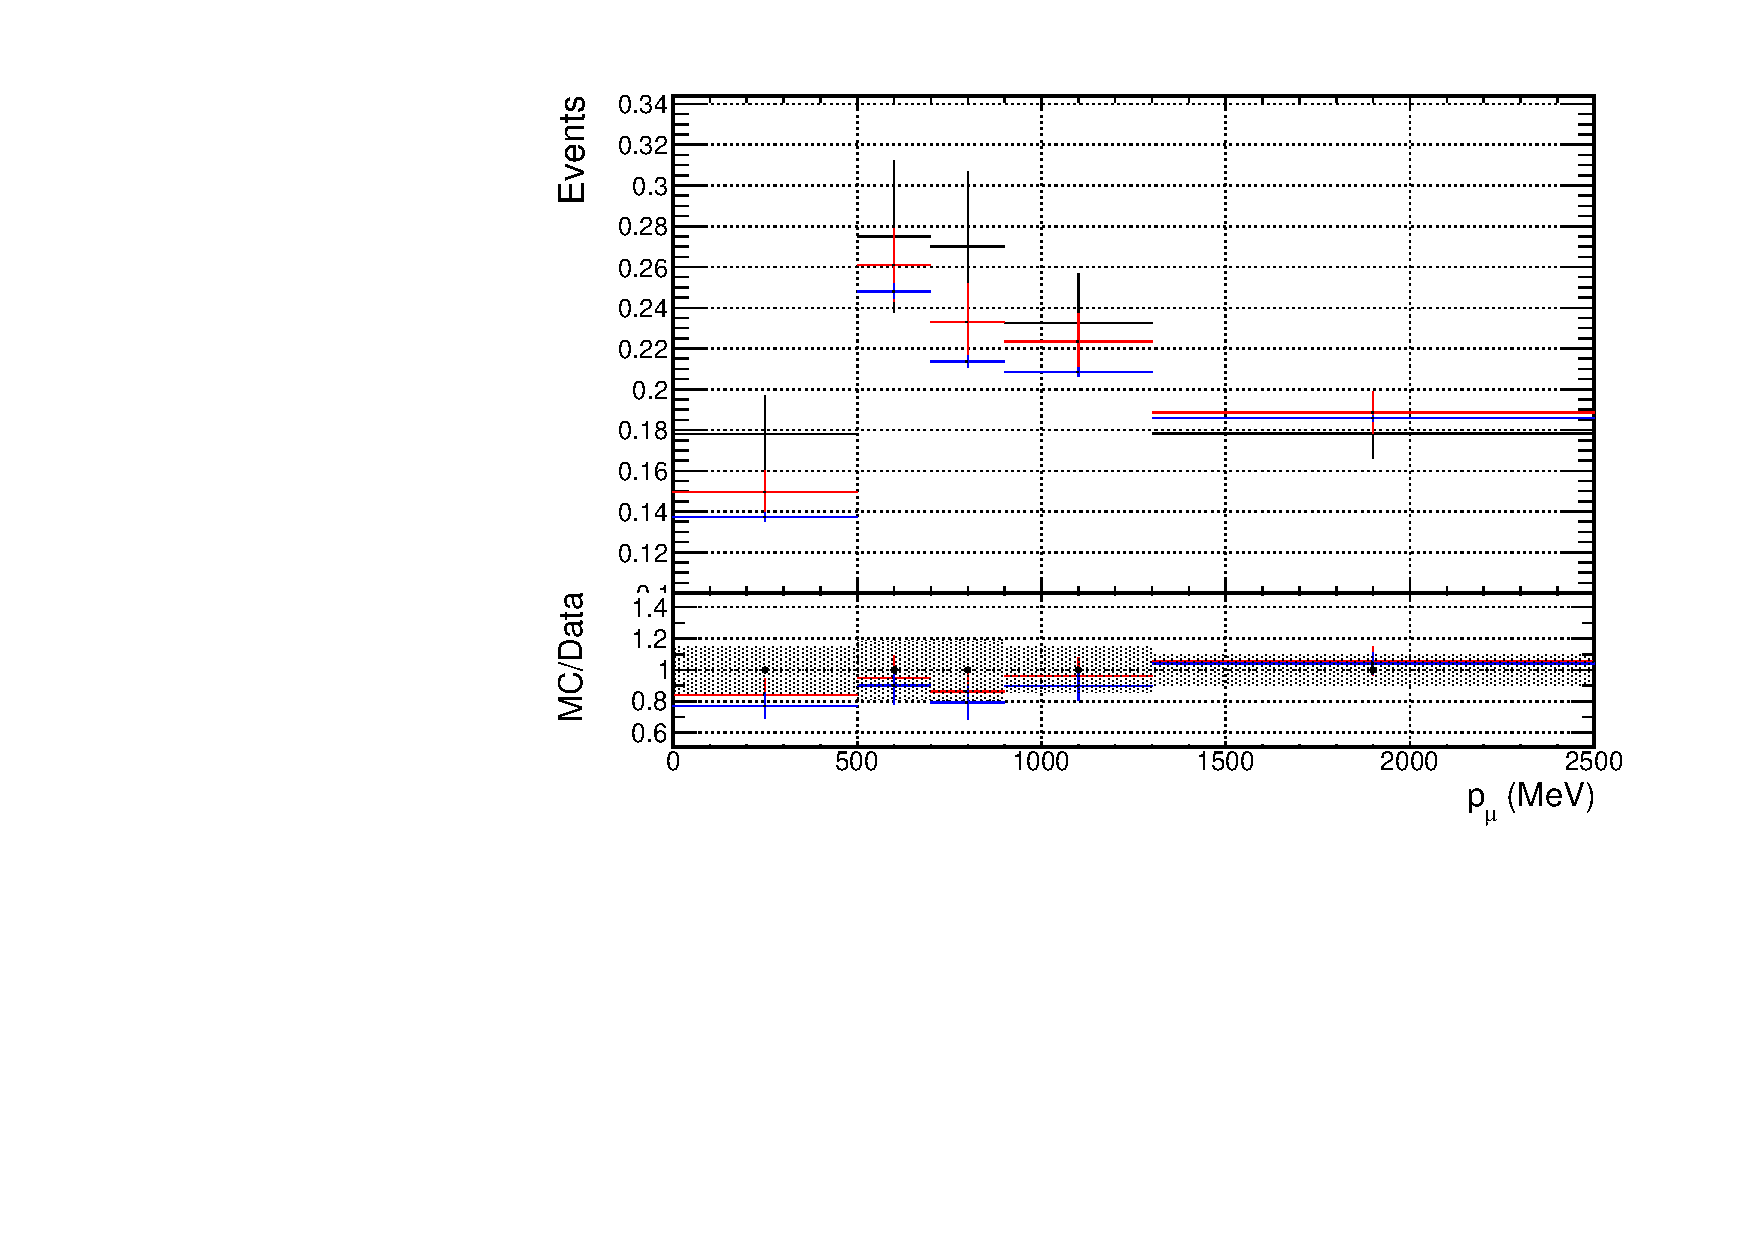
\includegraphics[width=\textwidth]{figs/priorpred1D_p_FGD2_anti-numuCC_1pi}
  \caption{FGD2 RHC $\bar{\nu_{\mu}}$ 1$\pi$}
\end{subfigure}

\begin{subfigure}{0.49\textwidth}
  \centering
  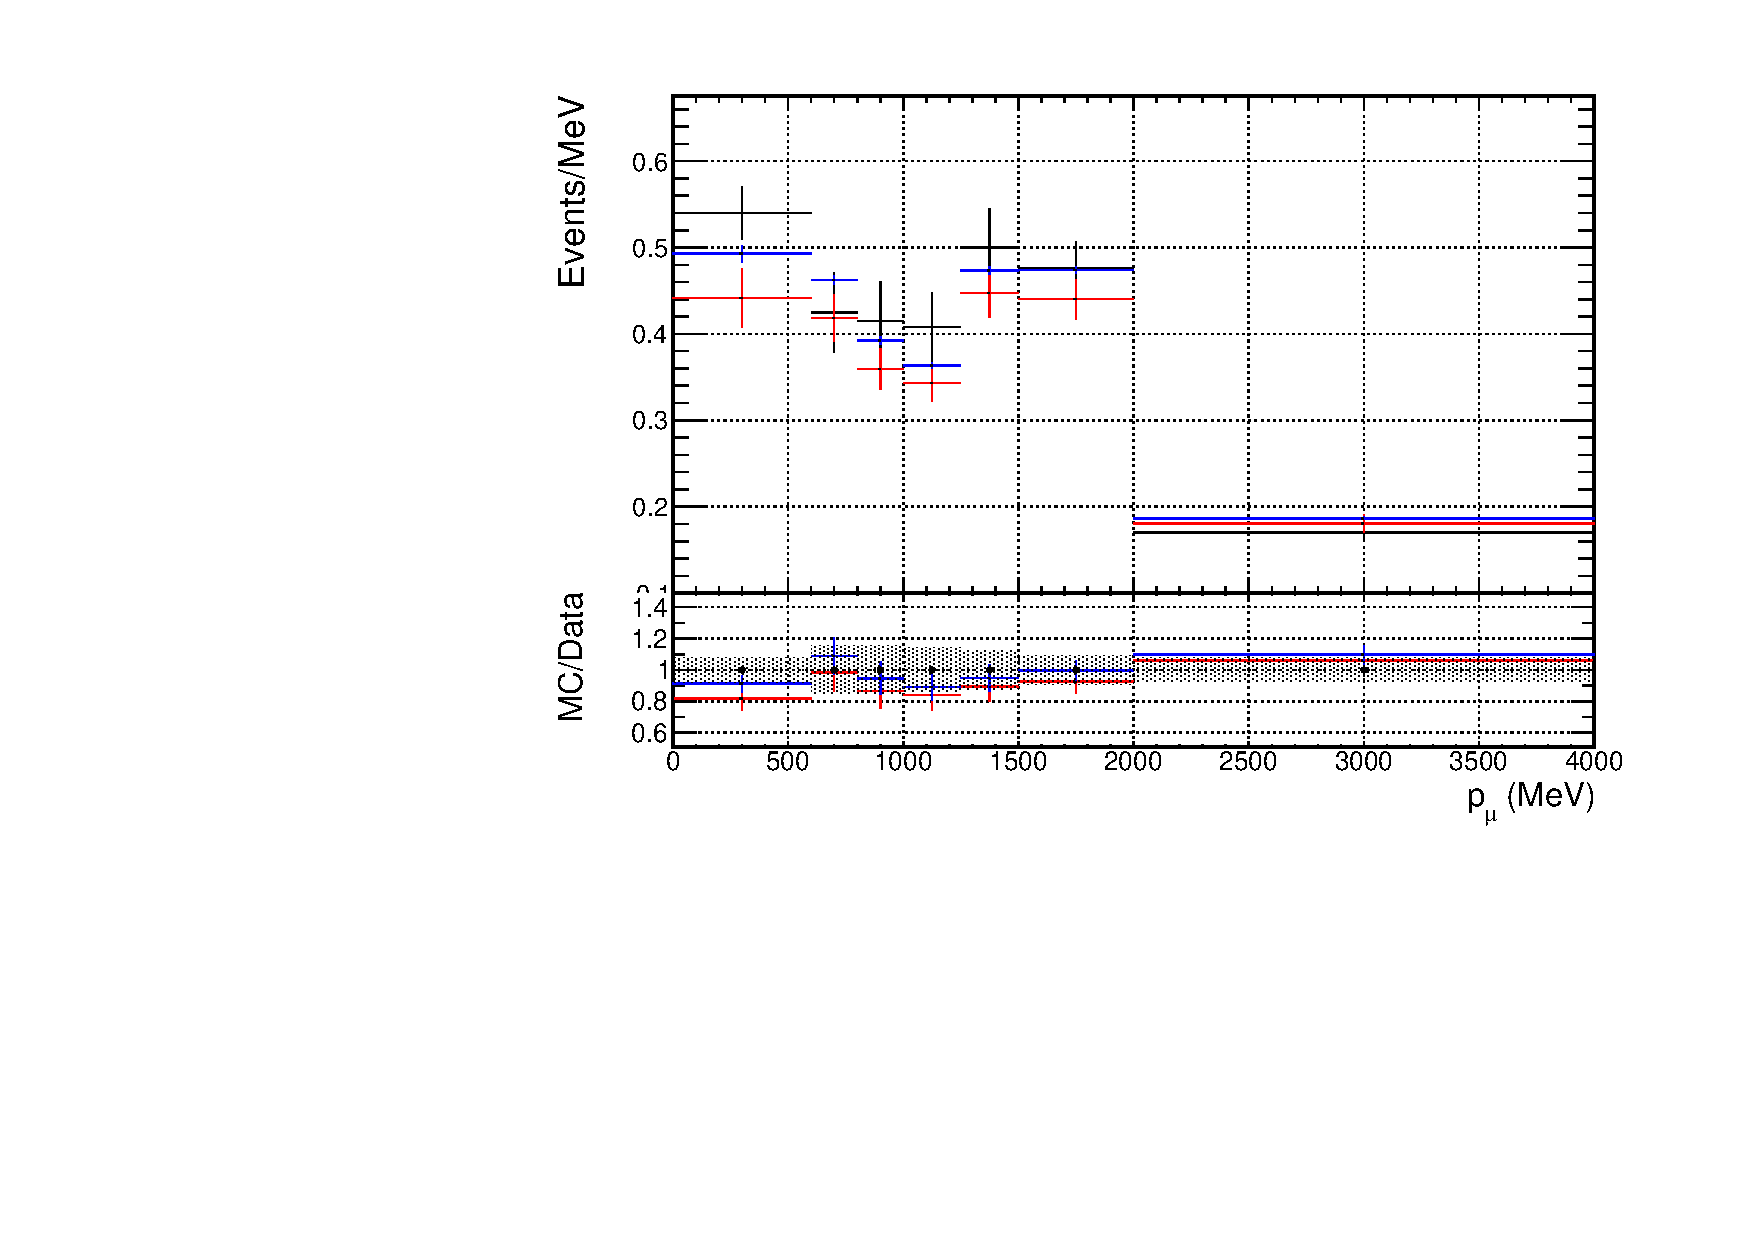
\includegraphics[width=\textwidth]{figs/priorpred1D_p_FGD1_anti-numuCC_other}
  \caption{FGD1 RHC $\bar{\nu_{\mu}}$ Other}
\end{subfigure}
\begin{subfigure}{0.49\textwidth}
  \centering
  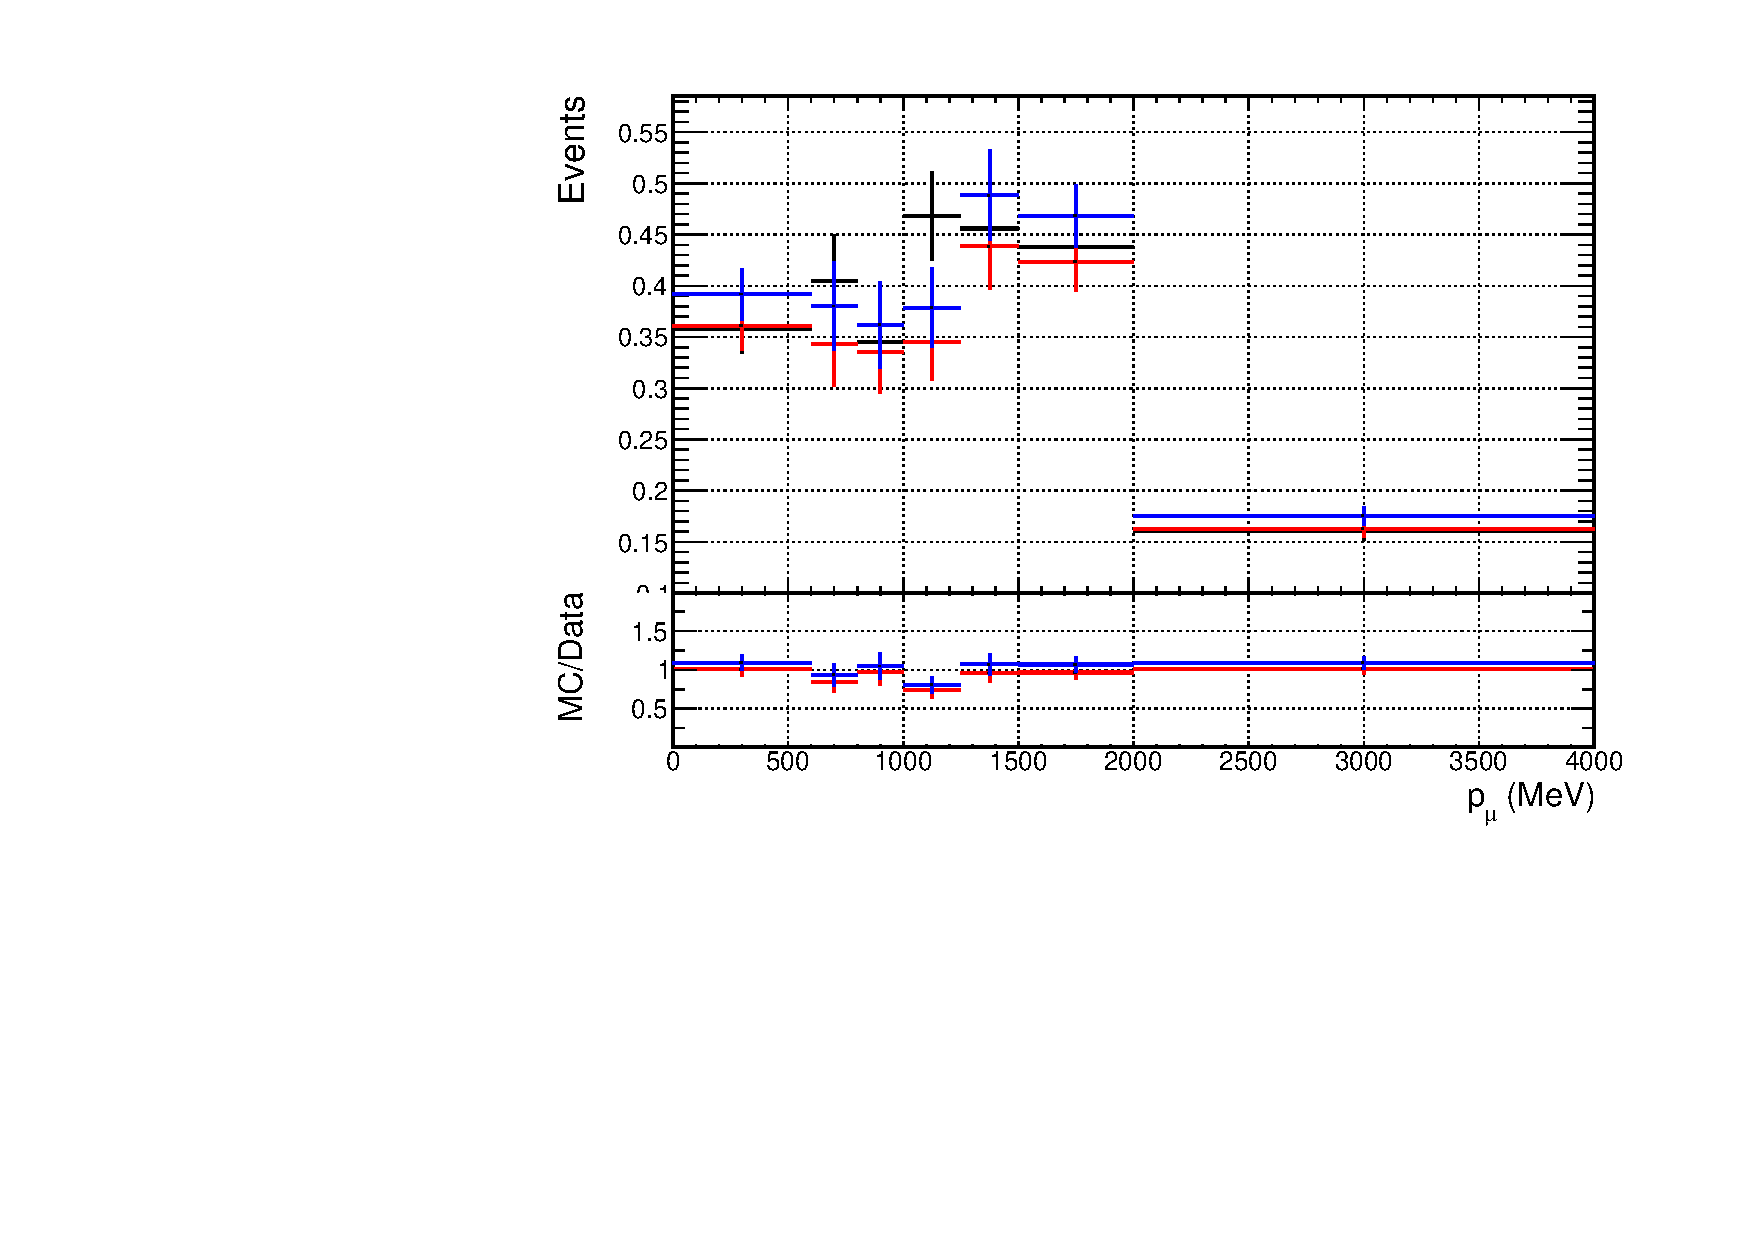
\includegraphics[width=\textwidth]{figs/priorpred1D_p_FGD2_anti-numuCC_other}
  \caption{FGD2 RHC $\bar{\nu_{\mu}}$ Other}
\end{subfigure}
\caption{$p_{\mu}$ projections of the prior and posterior predictive distributions and data for RHC \numub selections.}
\label{fig:priorpost_rhc_numub_papp}
\end{figure}

\begin{figure}[!htbp]
\centering
\begin{subfigure}{.24\textwidth}
  \centering
  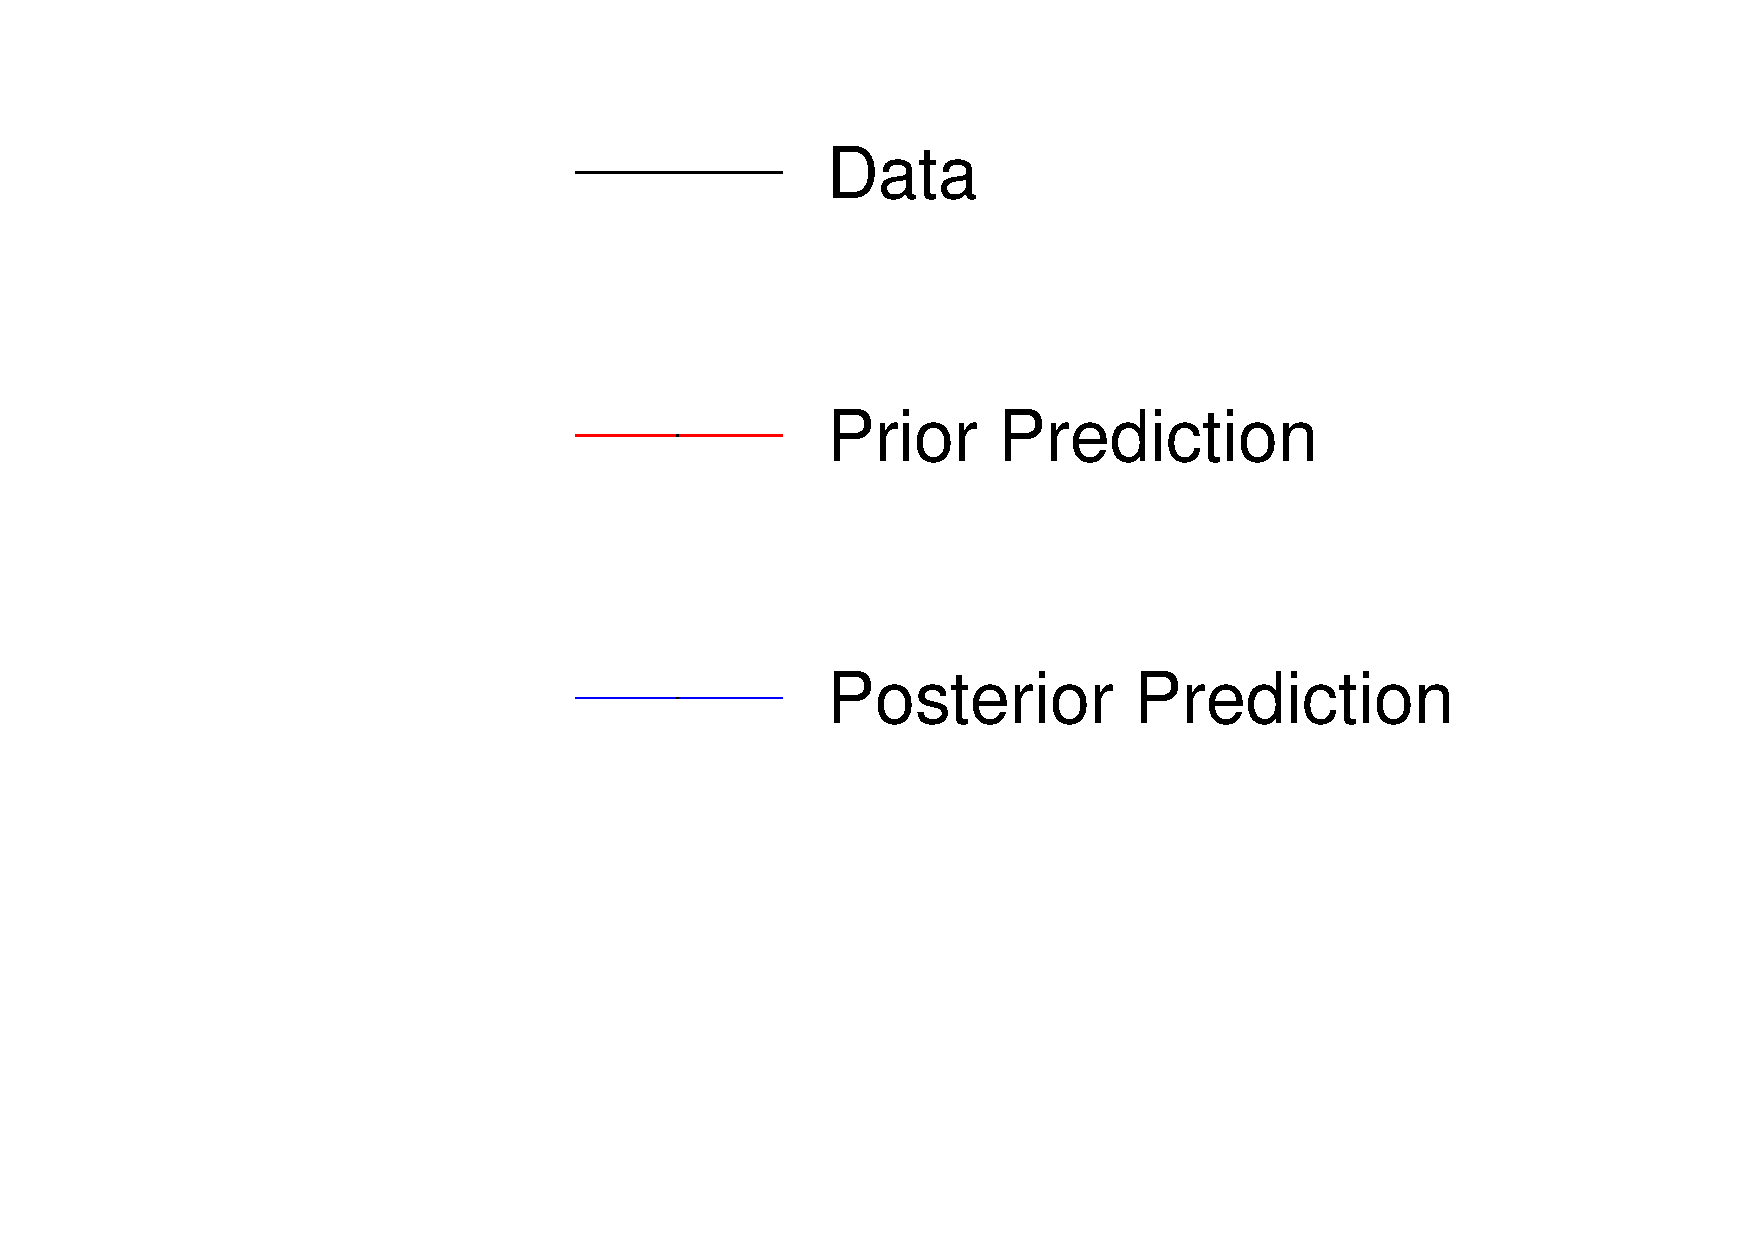
\includegraphics[width=\linewidth, clip]{figs/prior1dleg.pdf}
\end{subfigure}

\begin{subfigure}{0.49\textwidth}
  \centering
  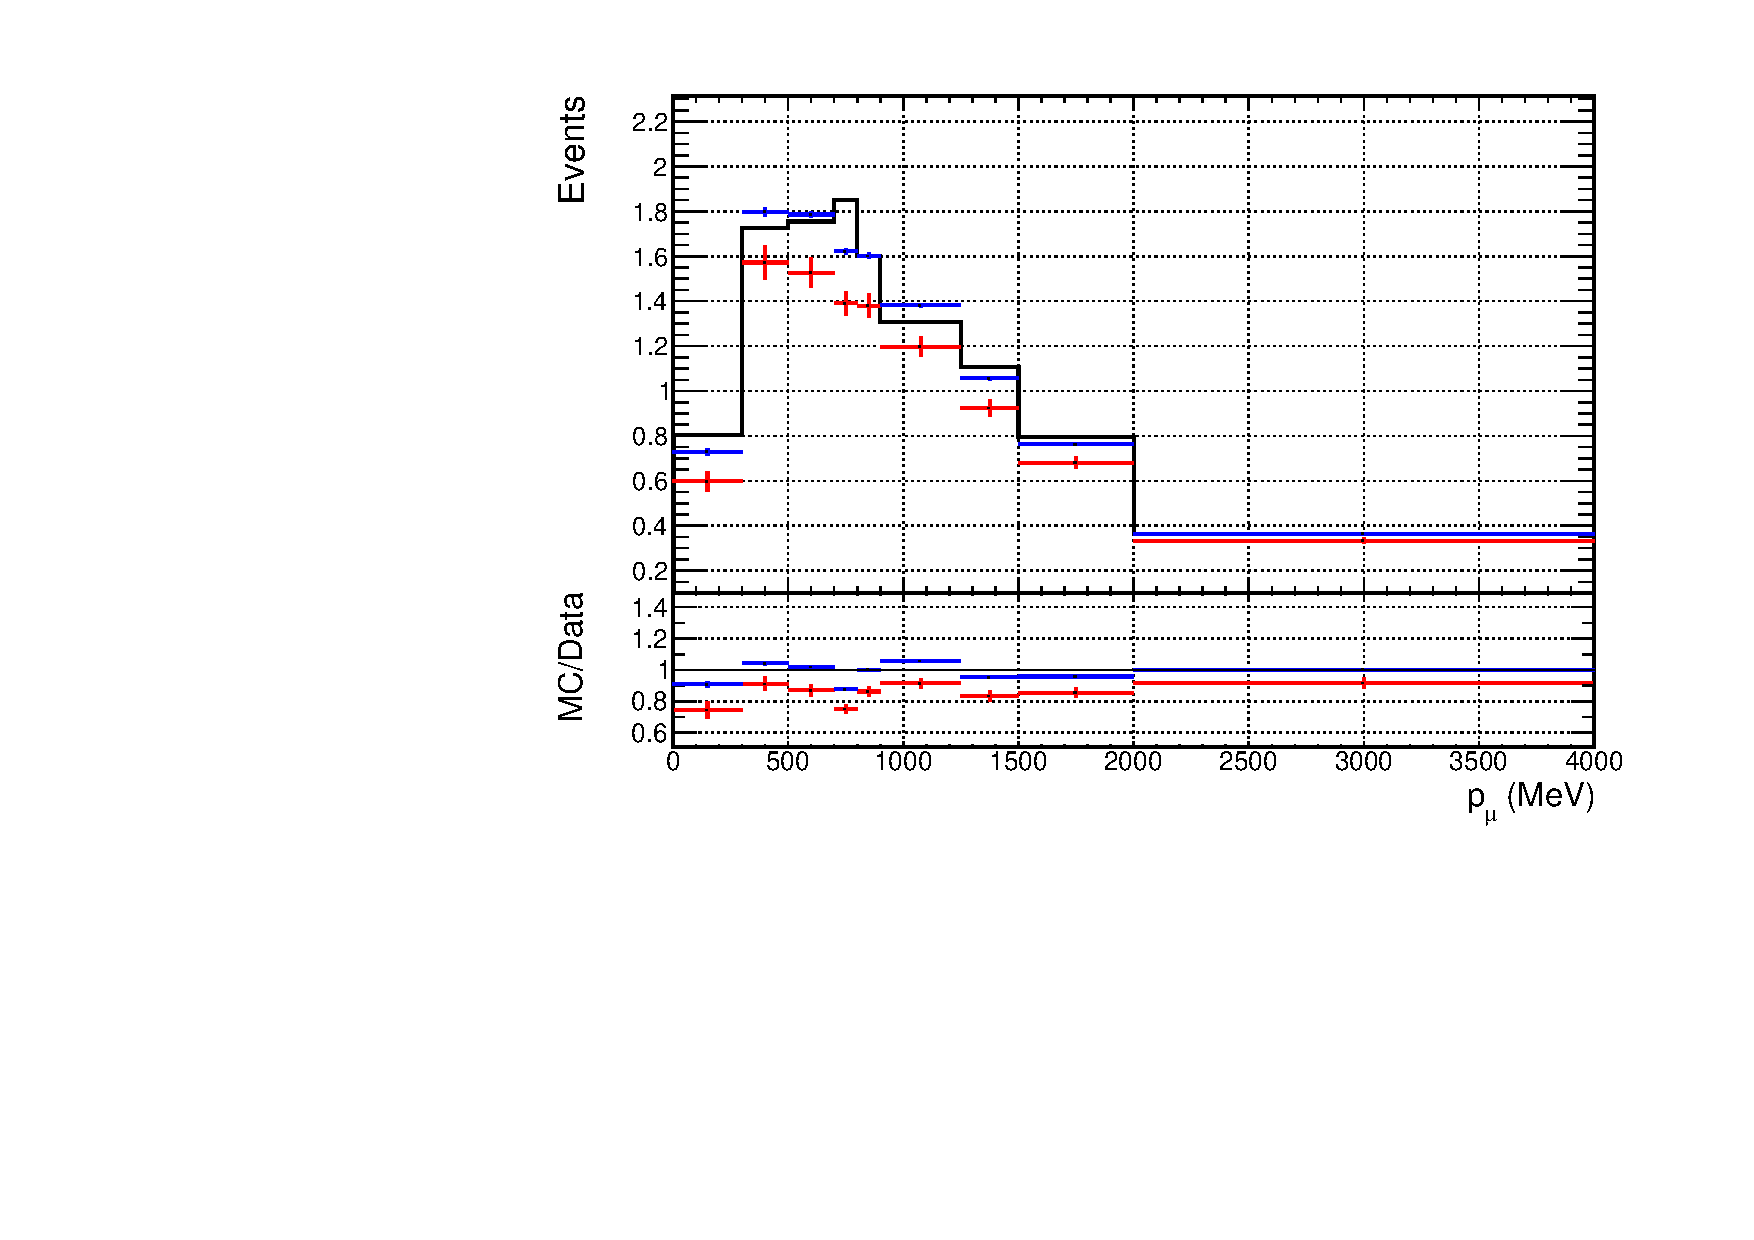
\includegraphics[width=\textwidth]{figs/priorpred1D_p_FGD1_NuMuBkg_CC0pi_in_AntiNu_Mode}
  \caption{FGD1 RHC $\nu_{\mu}$ 0$\pi$}
\end{subfigure}
\begin{subfigure}{0.49\textwidth}
  \centering
  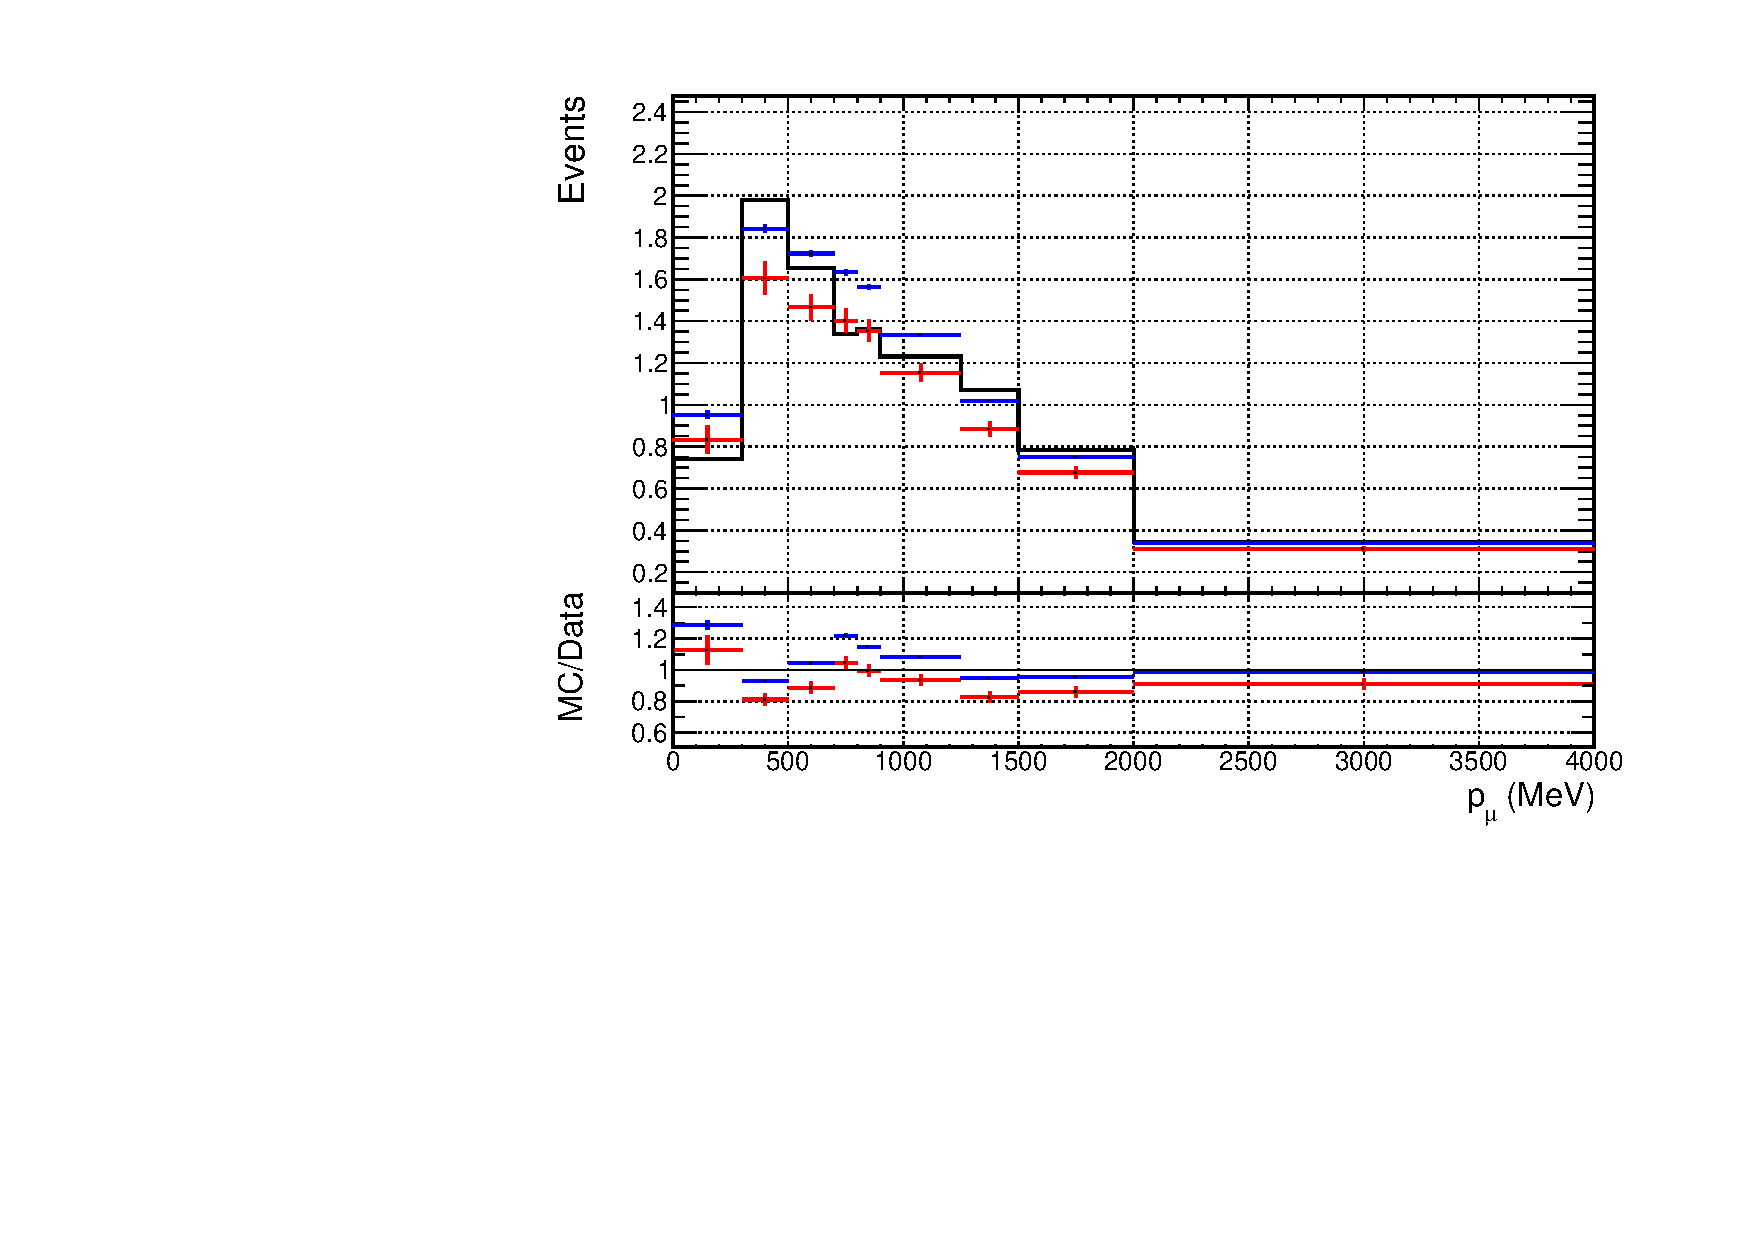
\includegraphics[width=\textwidth]{figs/priorpred1D_p_FGD2_NuMuBkg_CC0pi_in_AntiNu_Mode}
  \caption{FGD2 RHC $\nu_{\mu}$ 0$\pi$}
\end{subfigure}

\begin{subfigure}{0.49\textwidth}
  \centering
  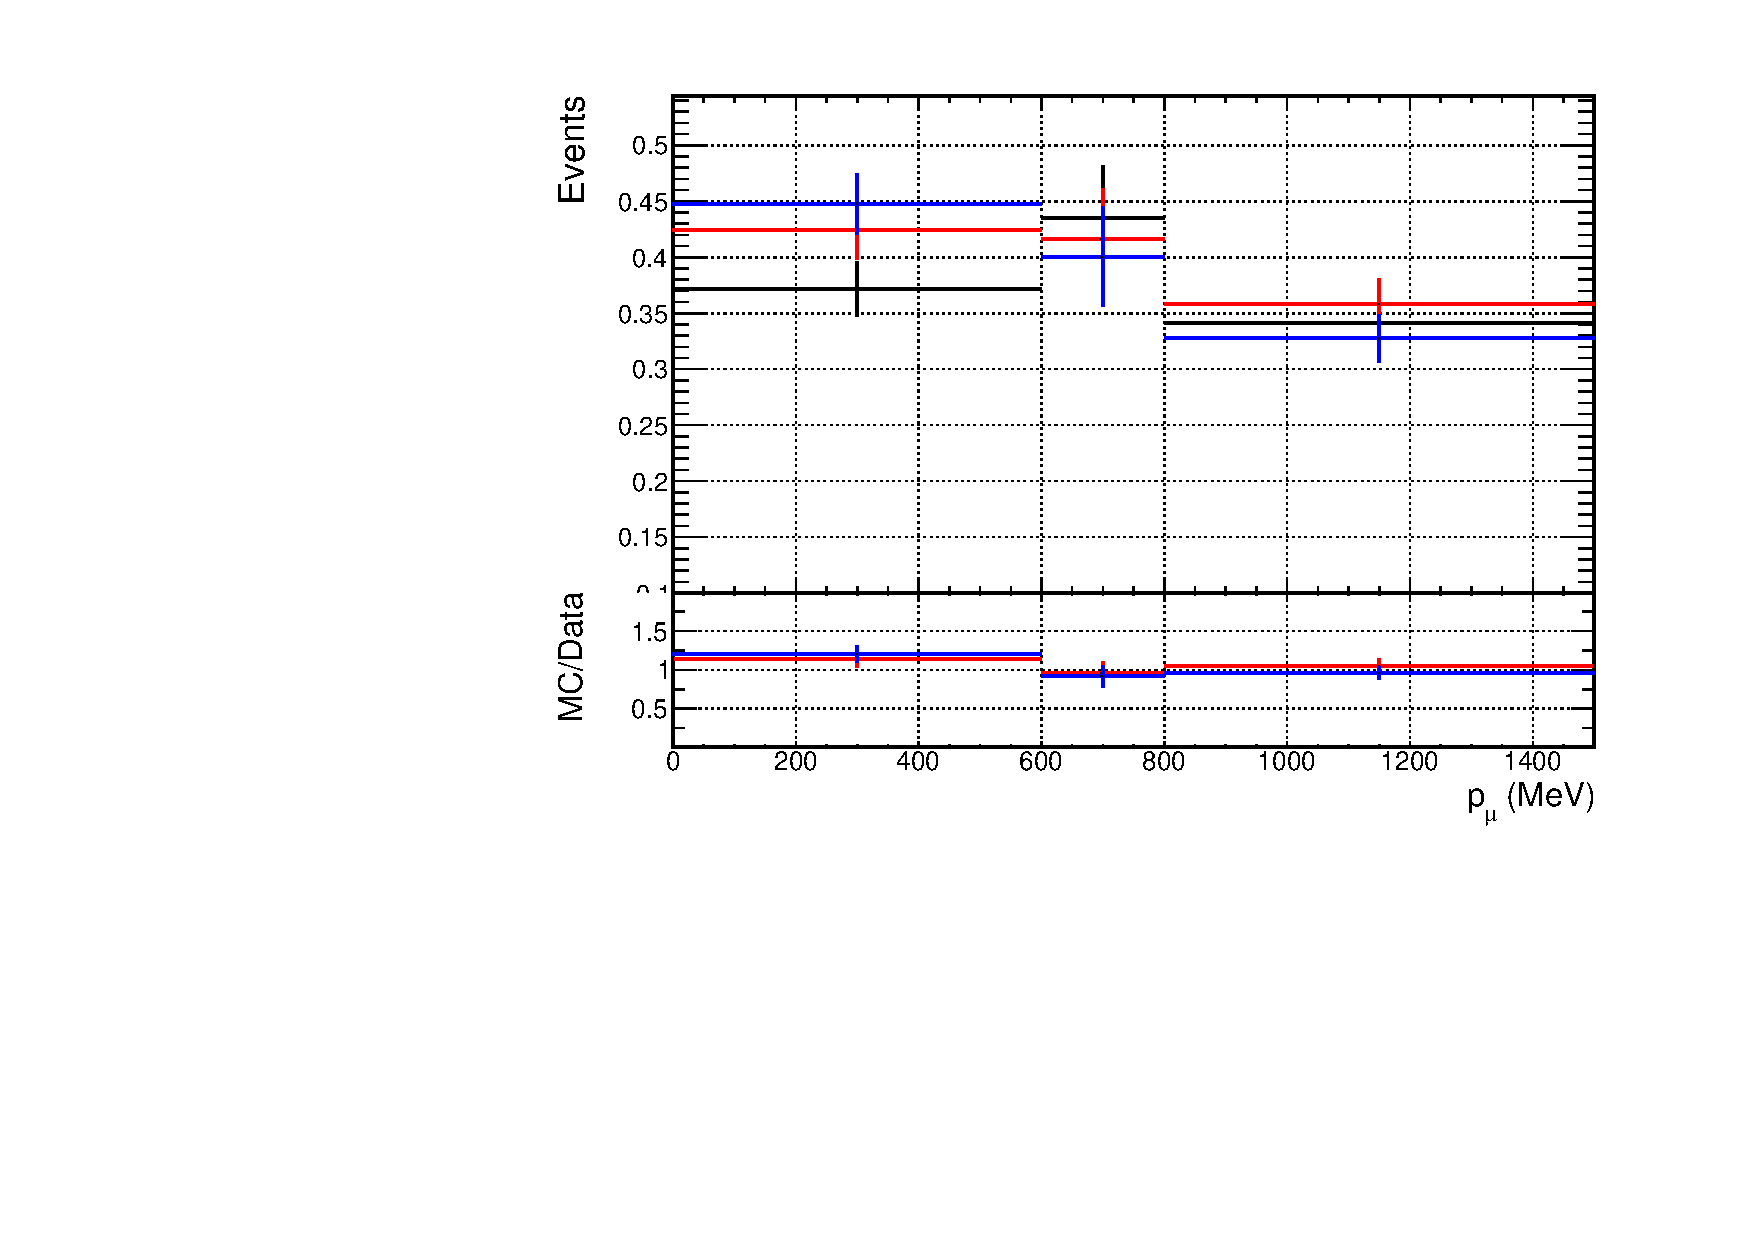
\includegraphics[width=\textwidth]{figs/priorpred1D_p_FGD1_NuMuBkg_CC1pi_in_AntiNu_Mode}
  \caption{FGD1 RHC $\nu_{\mu}$ 1$\pi$}
\end{subfigure}
\begin{subfigure}{0.49\textwidth}
  \centering
  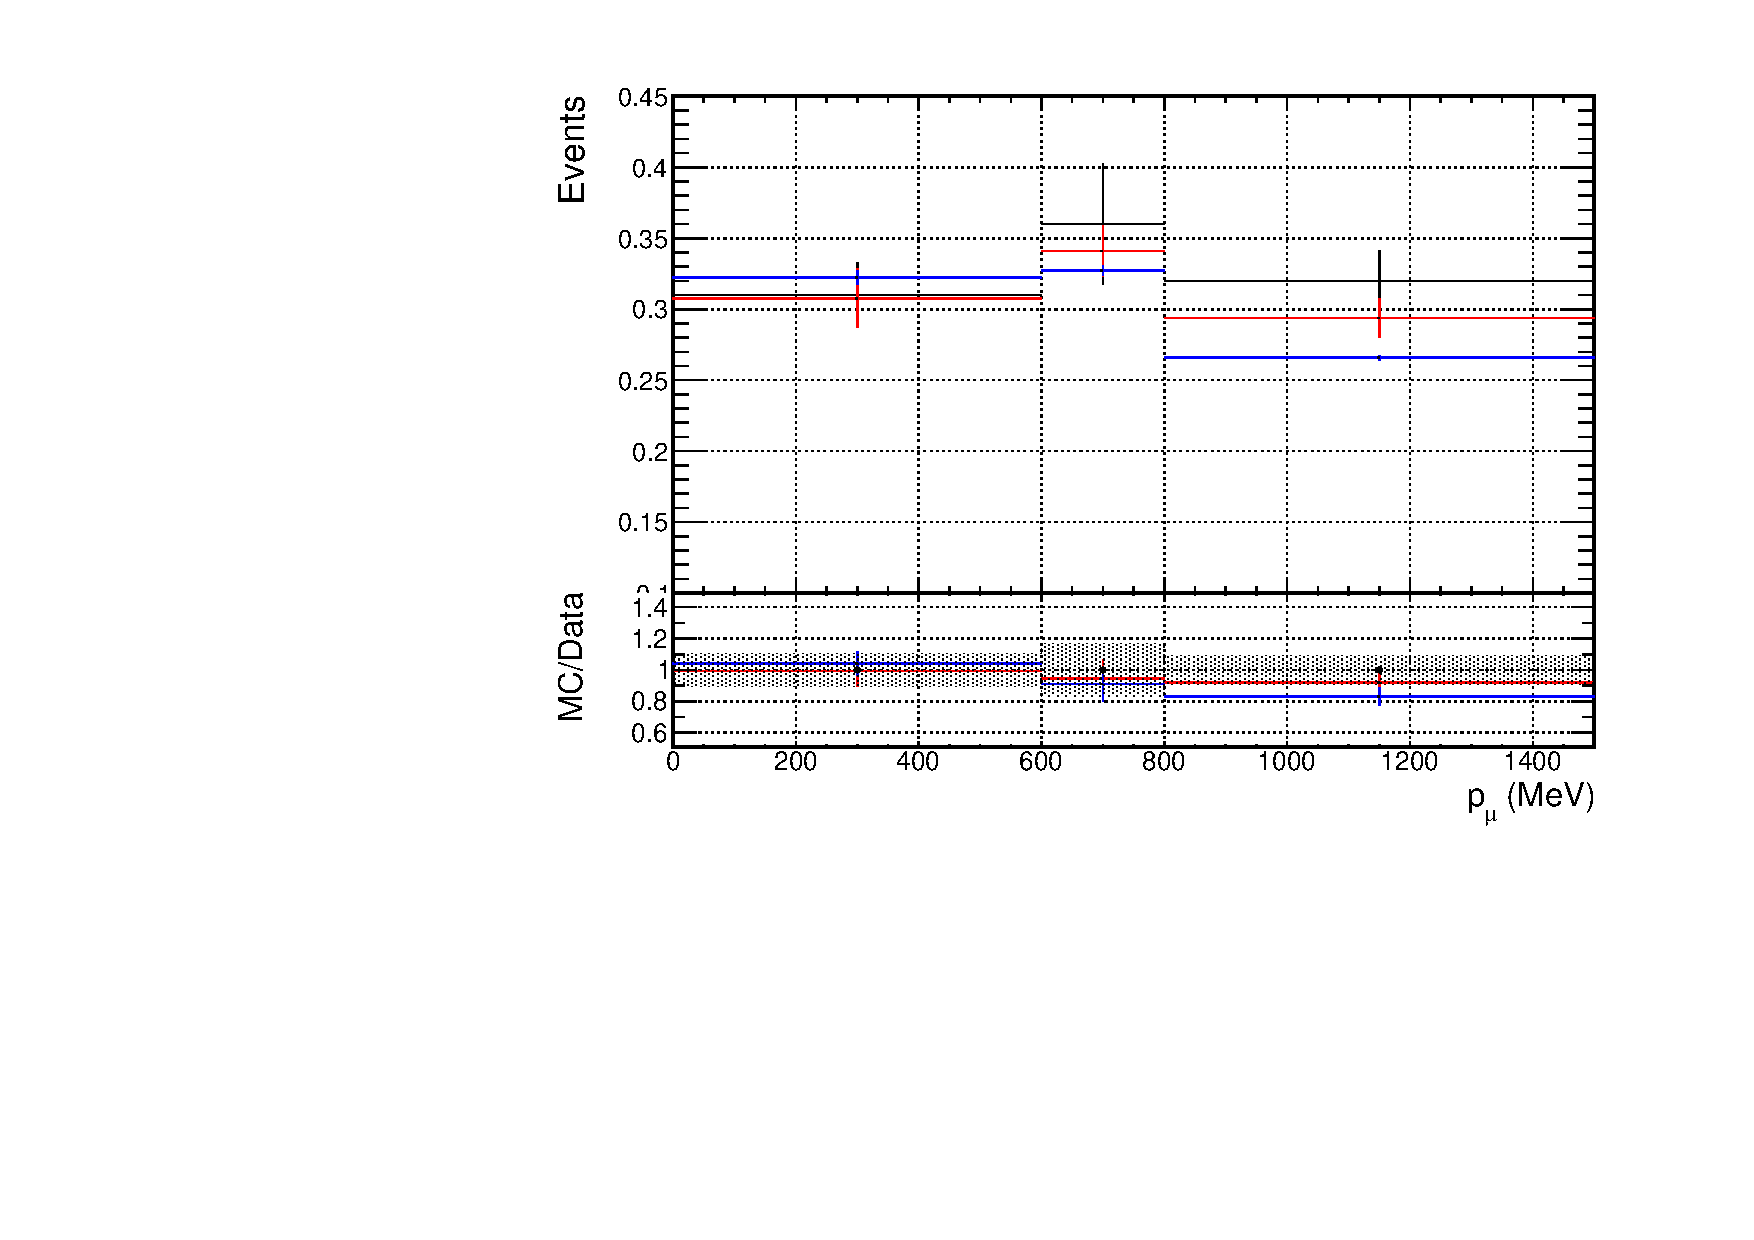
\includegraphics[width=\textwidth]{figs/priorpred1D_p_FGD2_NuMuBkg_CC1pi_in_AntiNu_Mode}
  \caption{FGD2 RHC $\nu_{\mu}$ 1$\pi$}
\end{subfigure}

\begin{subfigure}{0.49\textwidth}
  \centering
  \includegraphics[width=\textwidth]{figs/priorpred1D_p_FGD1_NuMuBkg_CCOther_in_AntiNu_Mode}
  \caption{FGD1 RHC $\nu_{\mu}$ Other}
\end{subfigure}
\begin{subfigure}{0.49\textwidth}
  \centering
  \includegraphics[width=\textwidth]{figs/priorpred1D_p_FGD2_NuMuBkg_CCOther_in_AntiNu_Mode}
  \caption{FGD2 RHC $\nu_{\mu}$ Other}
\end{subfigure}
\caption{$p_{\mu}$ projections of the prior and posterior predictive distributions and data for RHC \numu selections.}
\label{fig:priorpost_rhc_numu_papp}
\end{figure}

\begin{figure}[!htbp]
\centering
\begin{subfigure}{.24\textwidth}
  \centering
  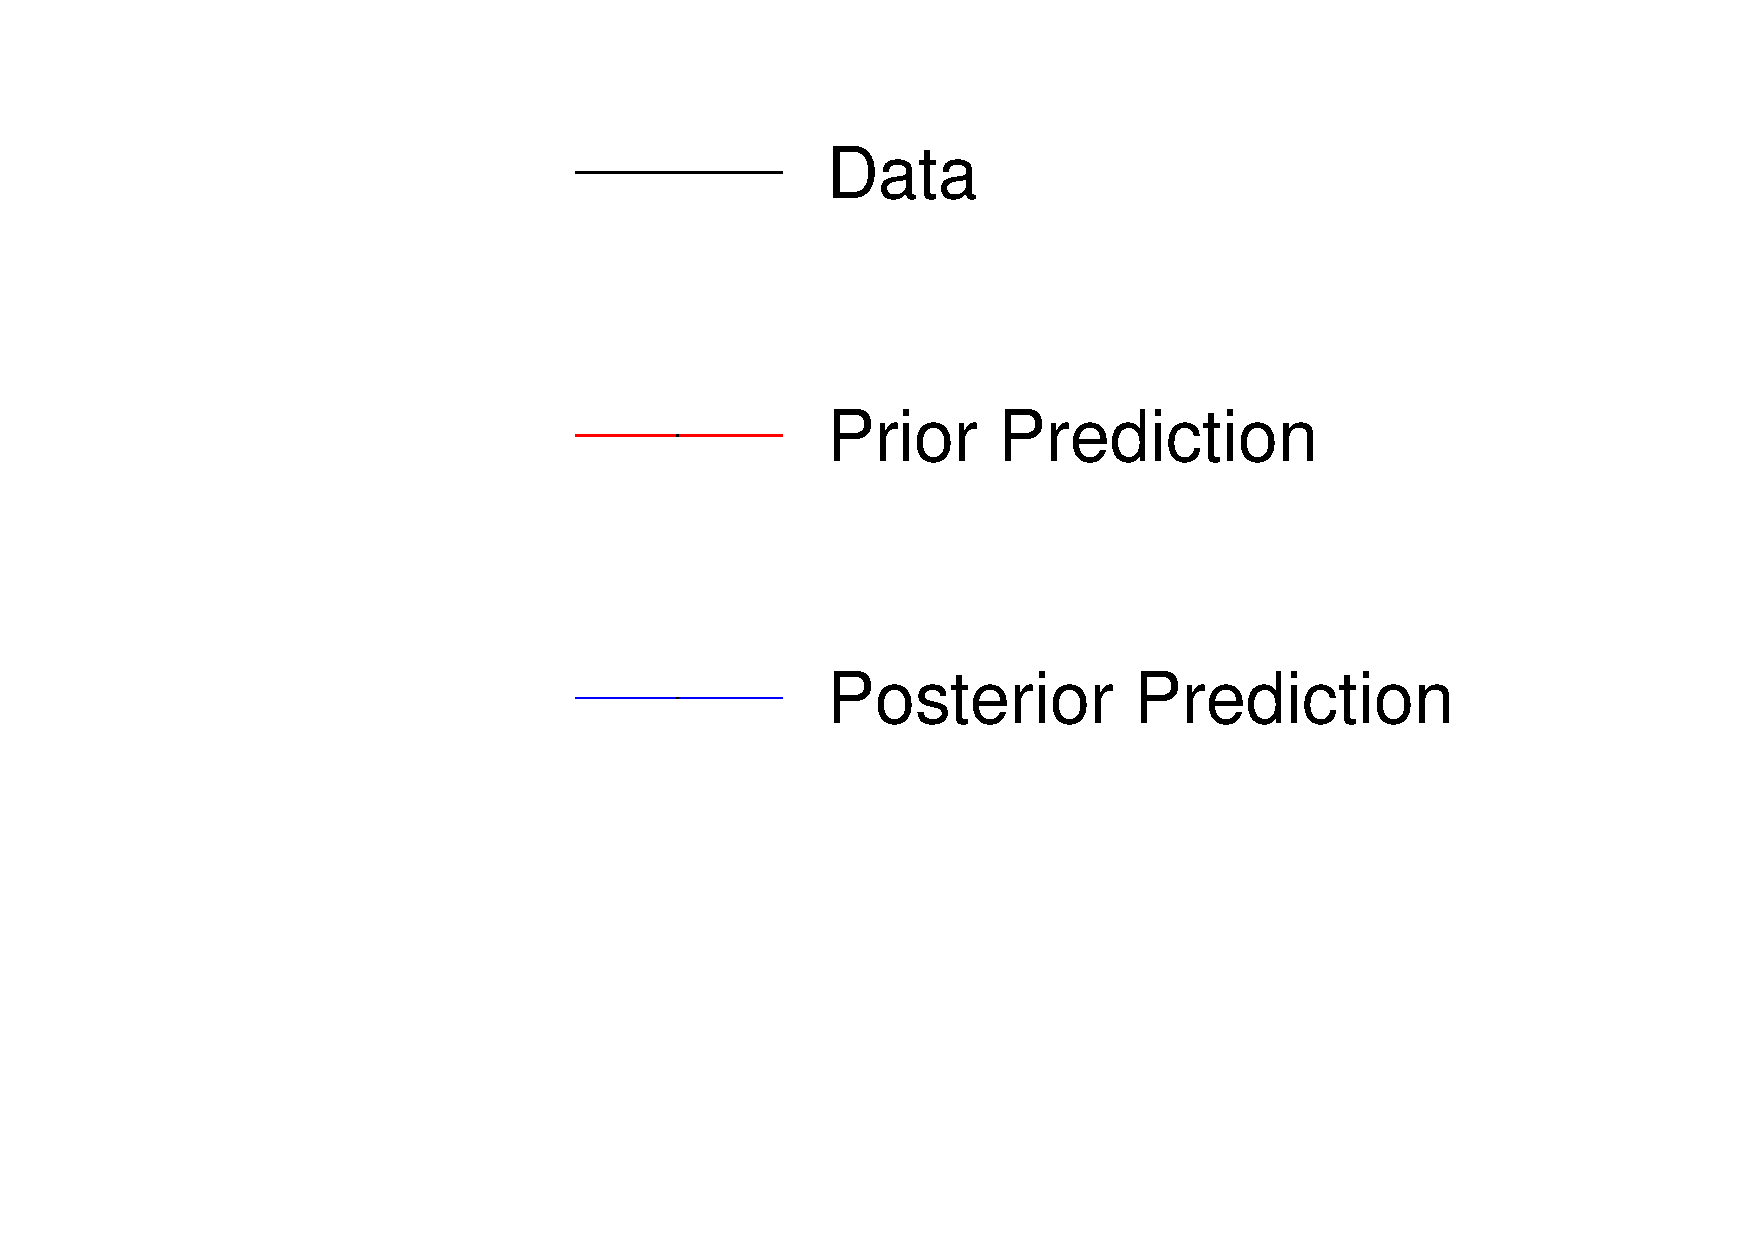
\includegraphics[width=\linewidth, clip]{figs/prior1dleg.pdf}
\end{subfigure}

\begin{subfigure}{0.49\textwidth}
  \centering
  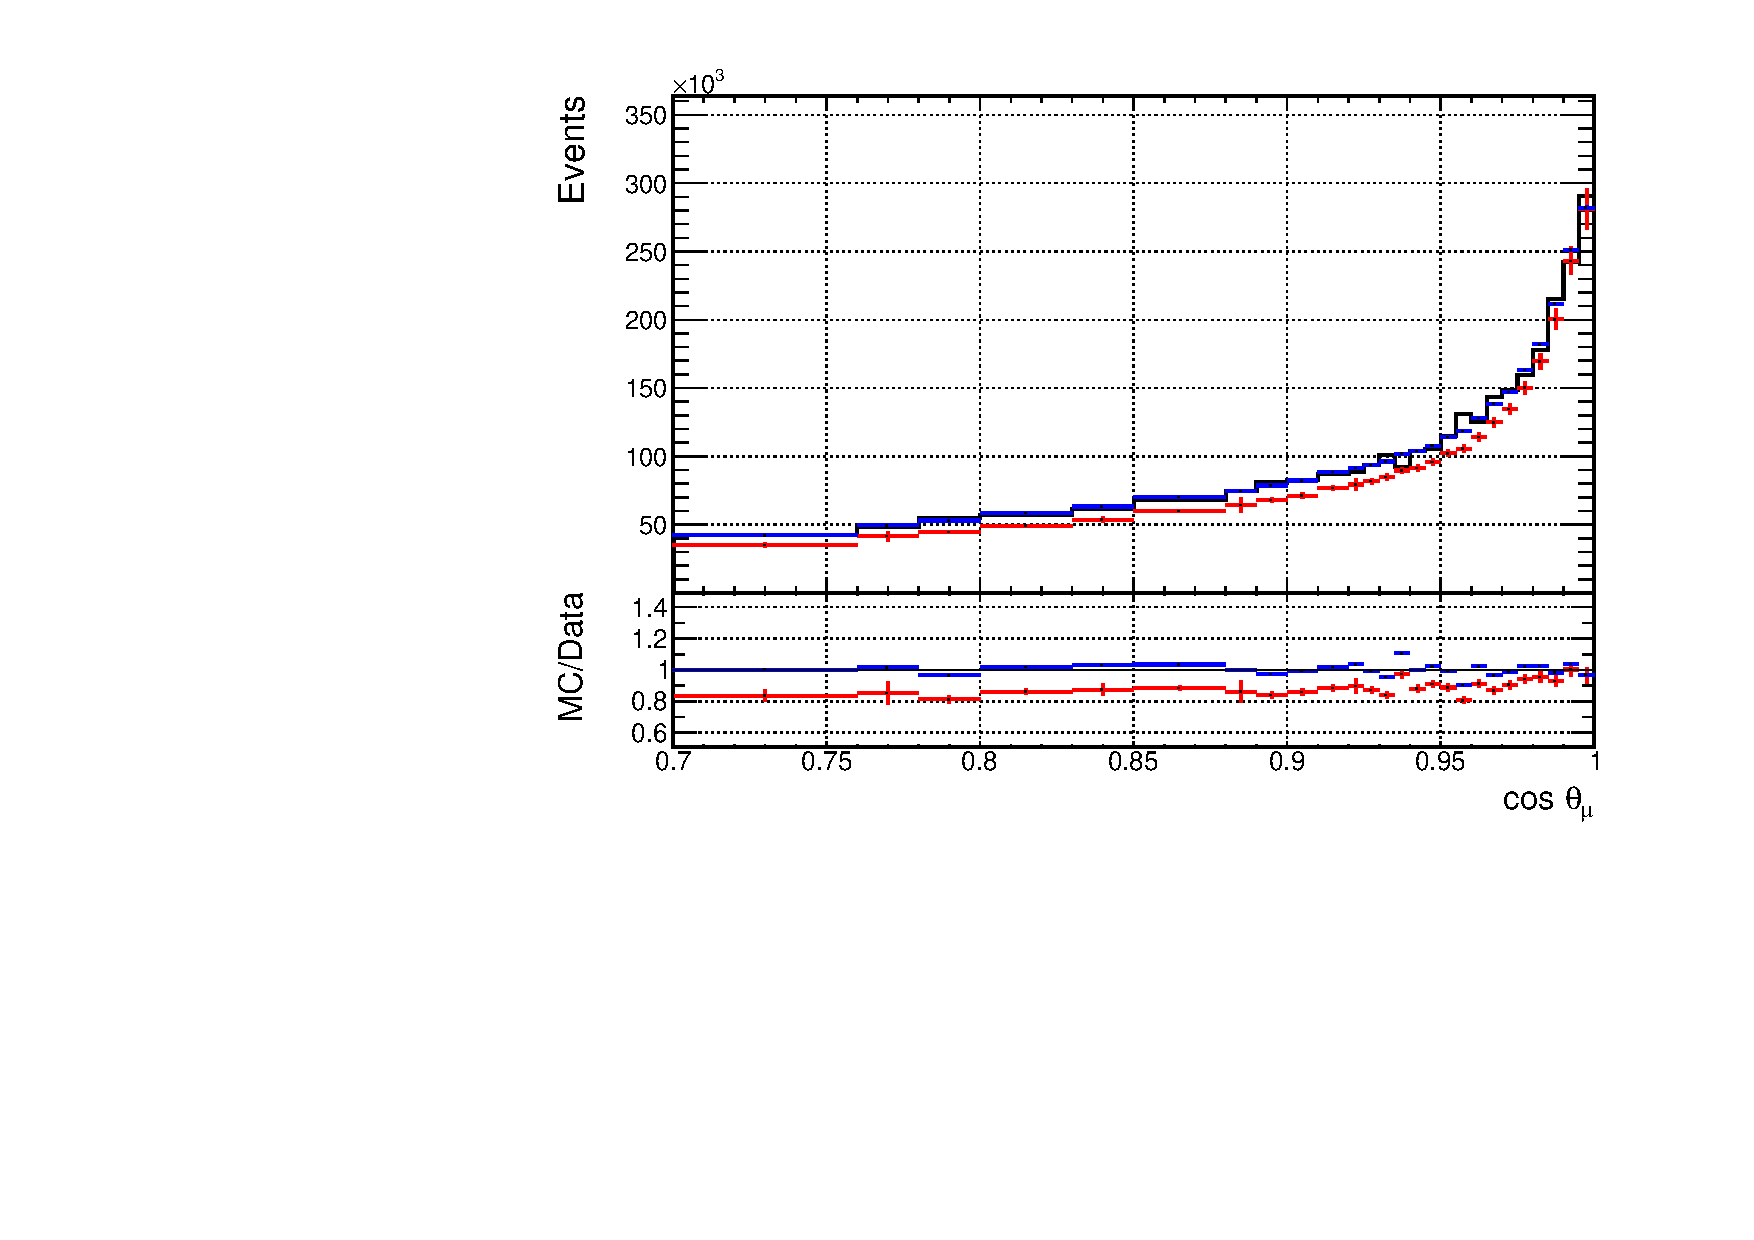
\includegraphics[width=\textwidth]{figs/priorpred1D_t_FGD1_numuCC_0pi}
  \caption{FGD1 FHC $\nu_{\mu}$ 0$\pi$}
\end{subfigure}
\begin{subfigure}{0.49\textwidth}
  \centering
  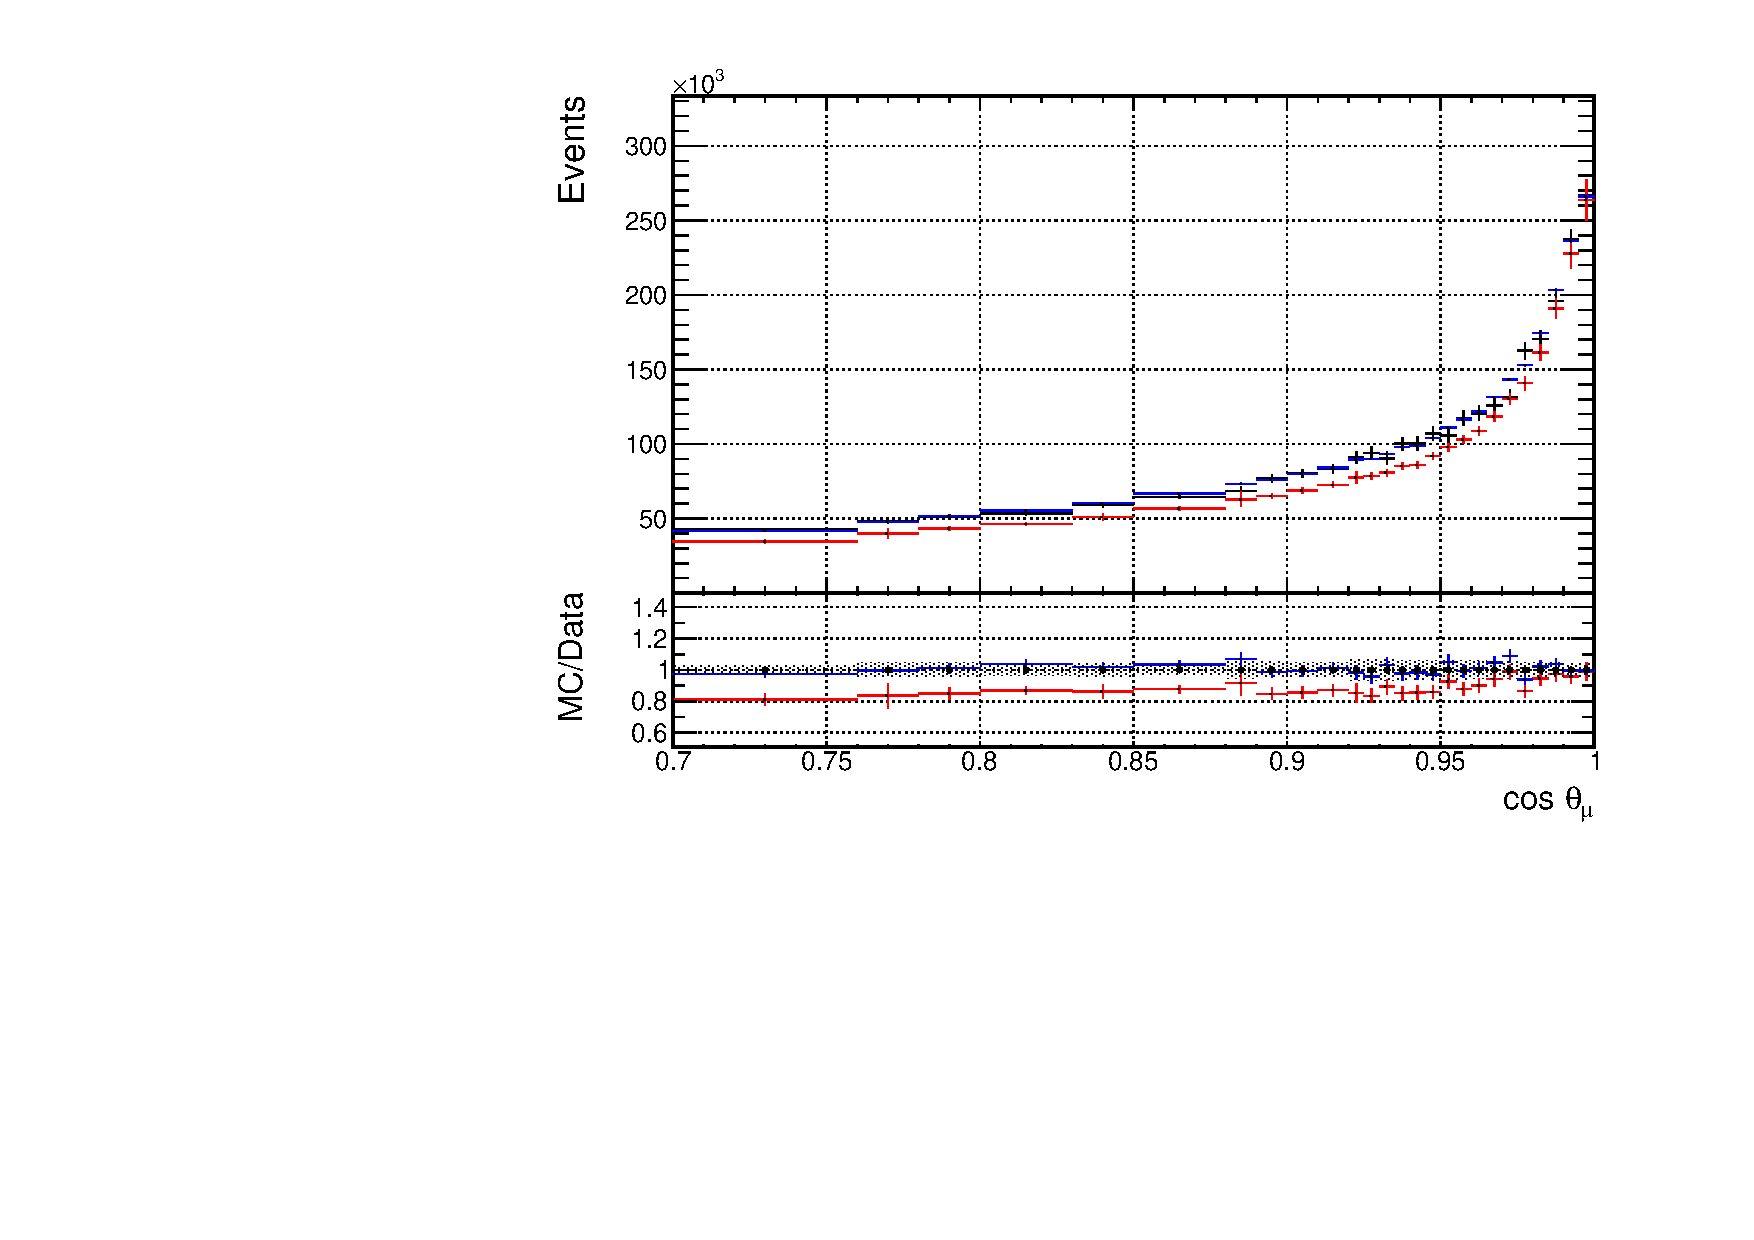
\includegraphics[width=\textwidth]{figs/priorpred1D_t_FGD2_numuCC_0pi}
  \caption{FGD2 FHC $\nu_{\mu}$ 0$\pi$}
\end{subfigure}

\begin{subfigure}{0.49\textwidth}
  \centering
  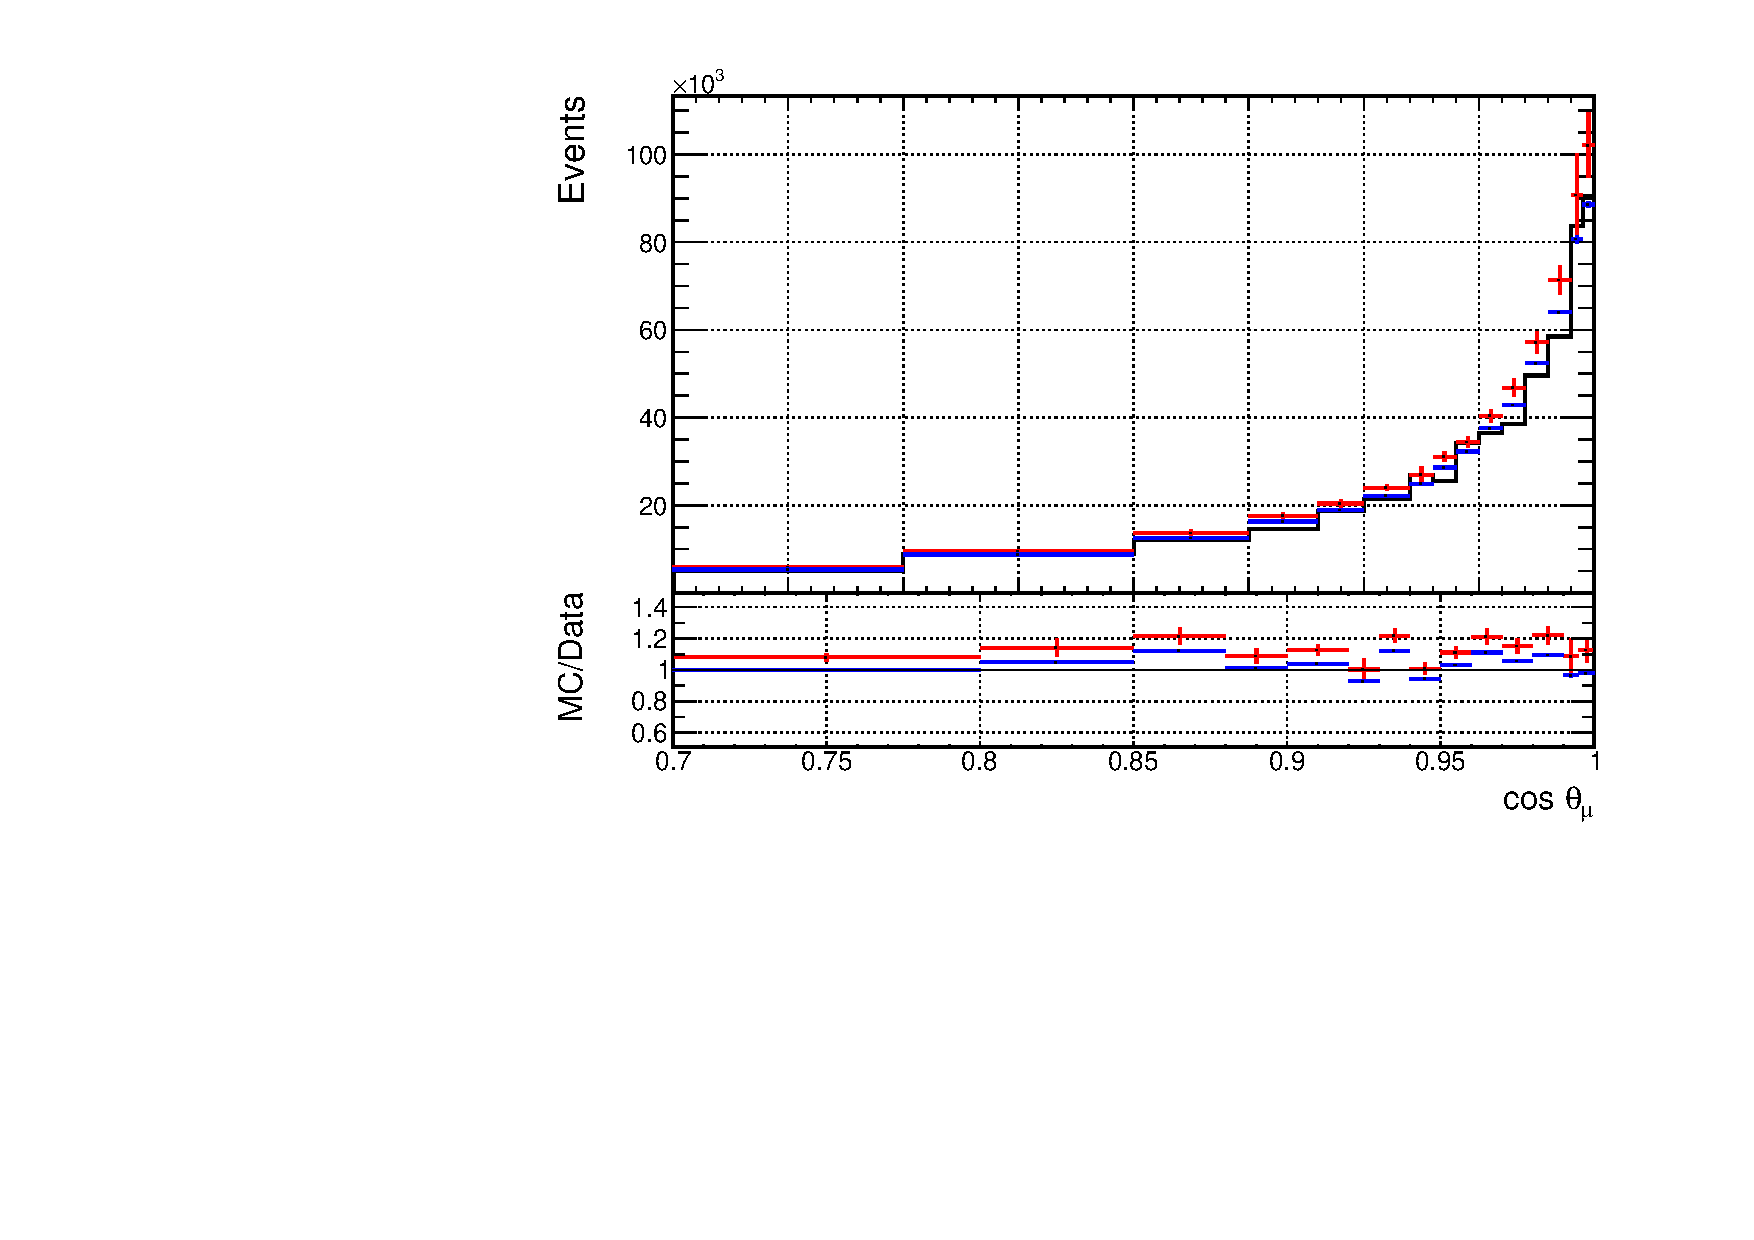
\includegraphics[width=\textwidth]{figs/priorpred1D_t_FGD1_numuCC_1pi}
  \caption{FGD1 FHC $\nu_{\mu}$ 1$\pi$}
\end{subfigure}
\begin{subfigure}{0.49\textwidth}
  \centering
  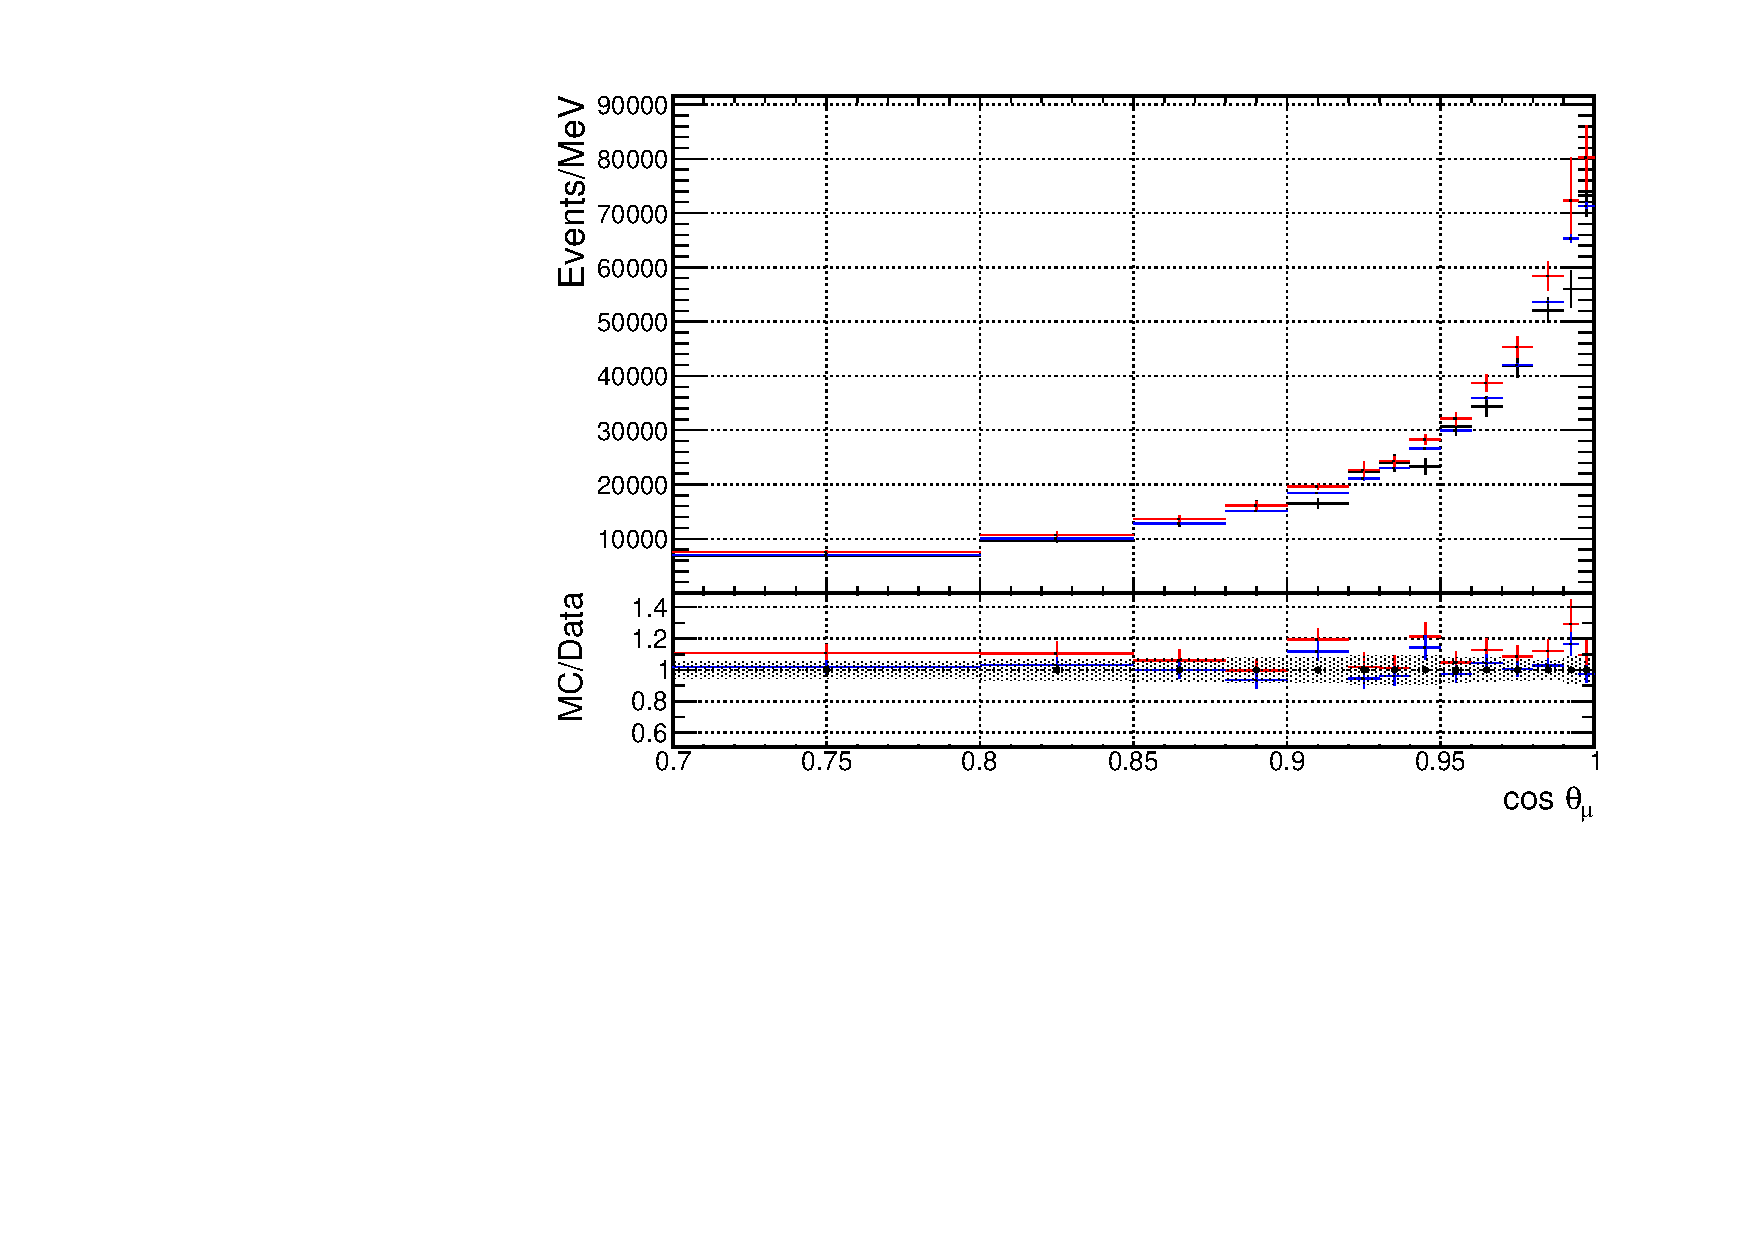
\includegraphics[width=\textwidth]{figs/priorpred1D_t_FGD2_numuCC_1pi}
  \caption{FGD2 FHC $\nu_{\mu}$ 1$\pi$}
\end{subfigure}

\begin{subfigure}{0.49\textwidth}
  \centering
  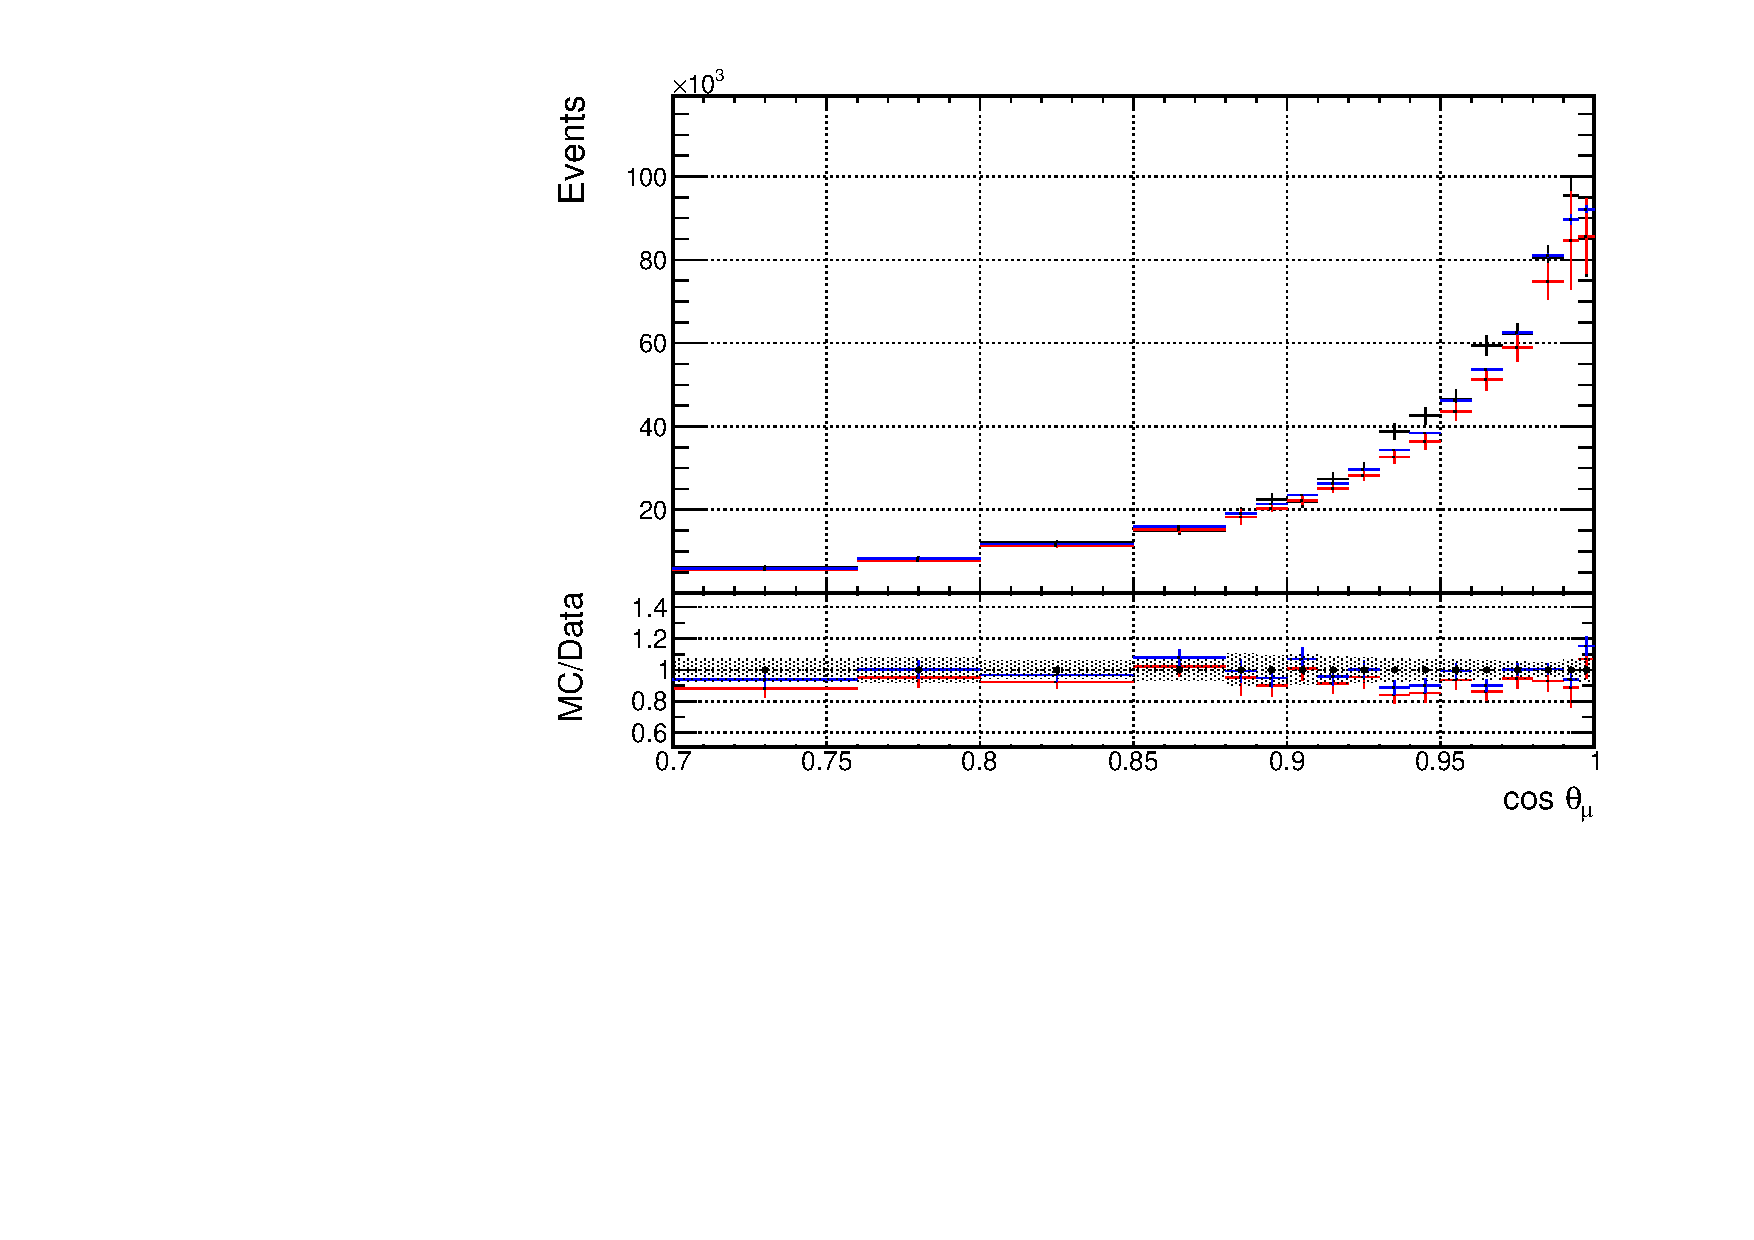
\includegraphics[width=\textwidth]{figs/priorpred1D_t_FGD1_numuCC_other}
  \caption{FGD1 FHC $\nu_{\mu}$ Other}
\end{subfigure}
\begin{subfigure}{0.49\textwidth}
  \centering
  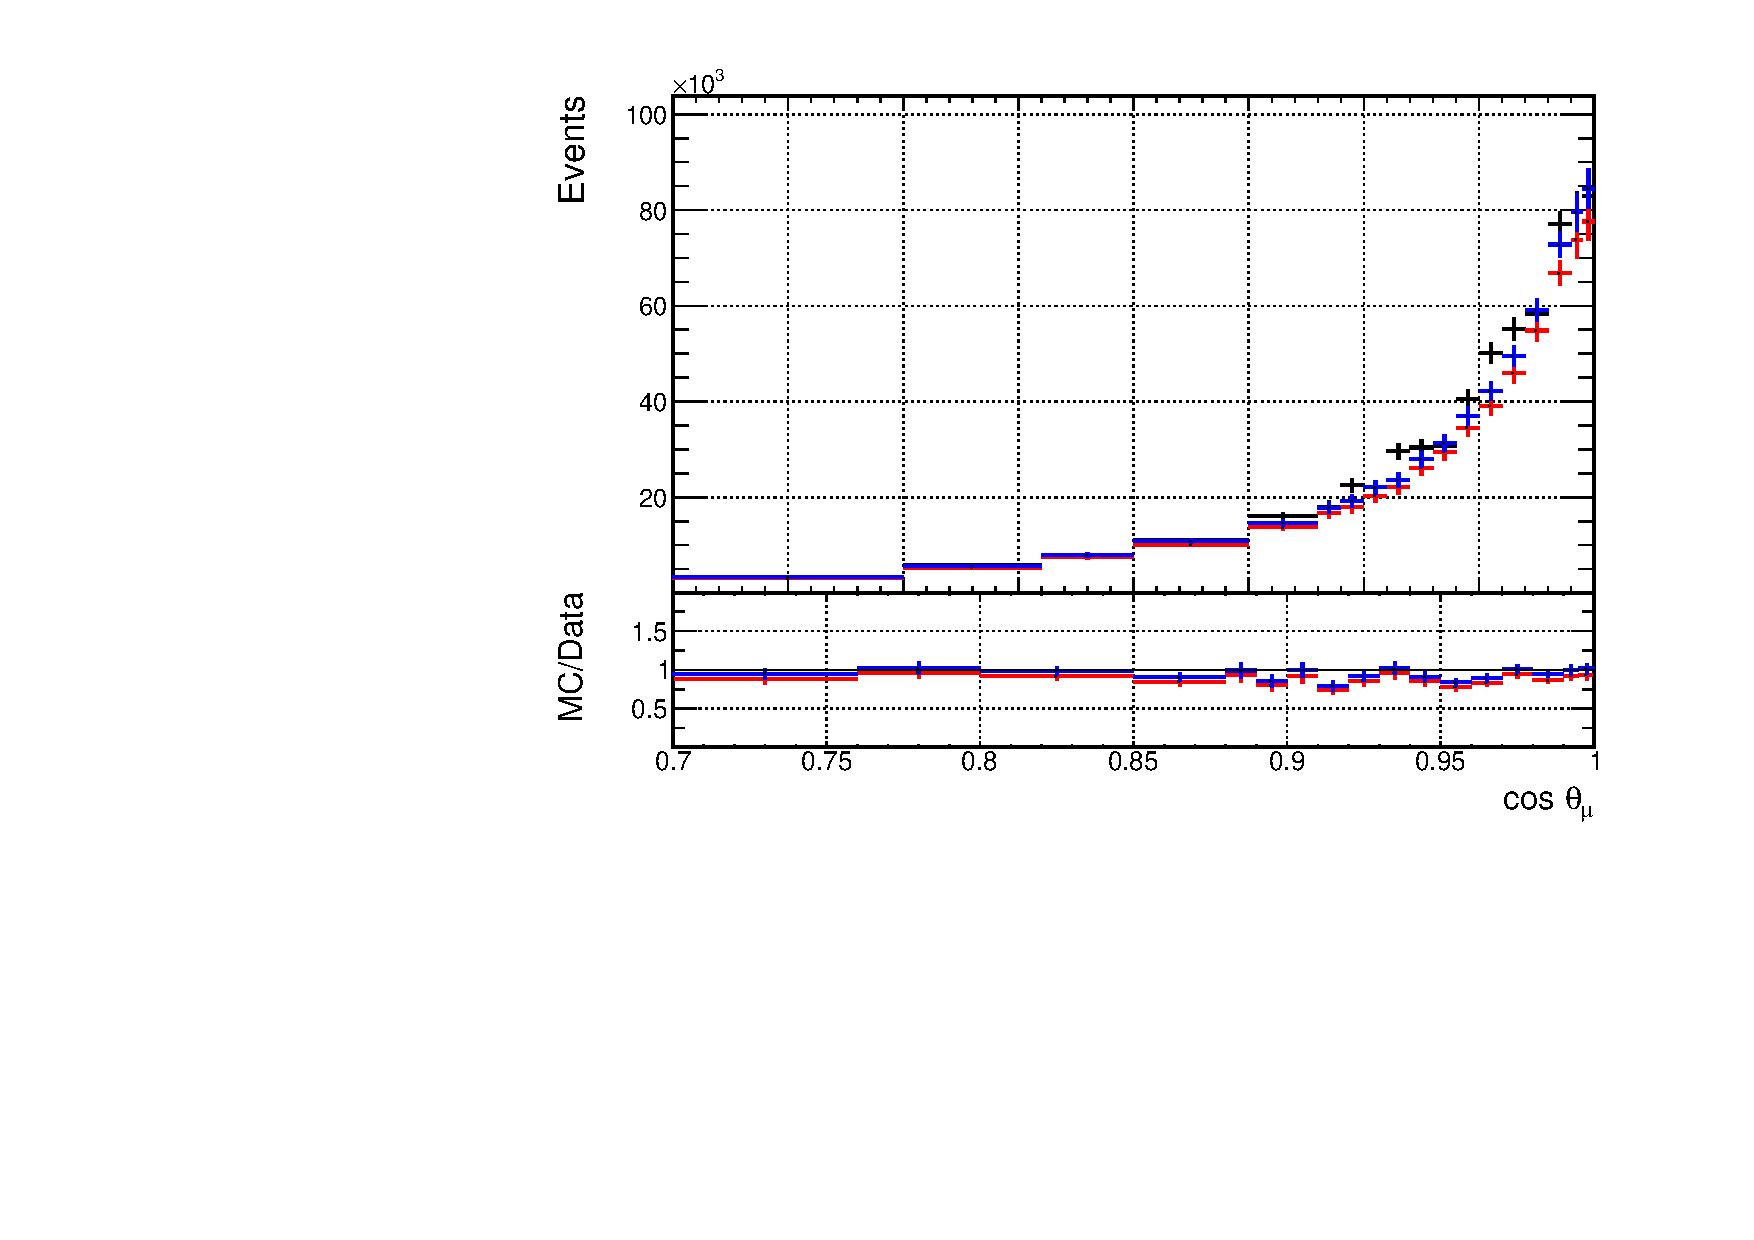
\includegraphics[width=\textwidth]{figs/priorpred1D_t_FGD2_numuCC_other}
  \caption{FGD2 FHC $\nu_{\mu}$ Other}
\end{subfigure}
\caption{cos$\theta_{\mu}$ projections of the prior and posterior predictive distributions and data for FHC \numu selections.}
\label{fig:priorpost_fhc_tapp}
\end{figure}

\begin{figure}[!htbp]
\centering
\begin{subfigure}{.24\textwidth}
  \centering
  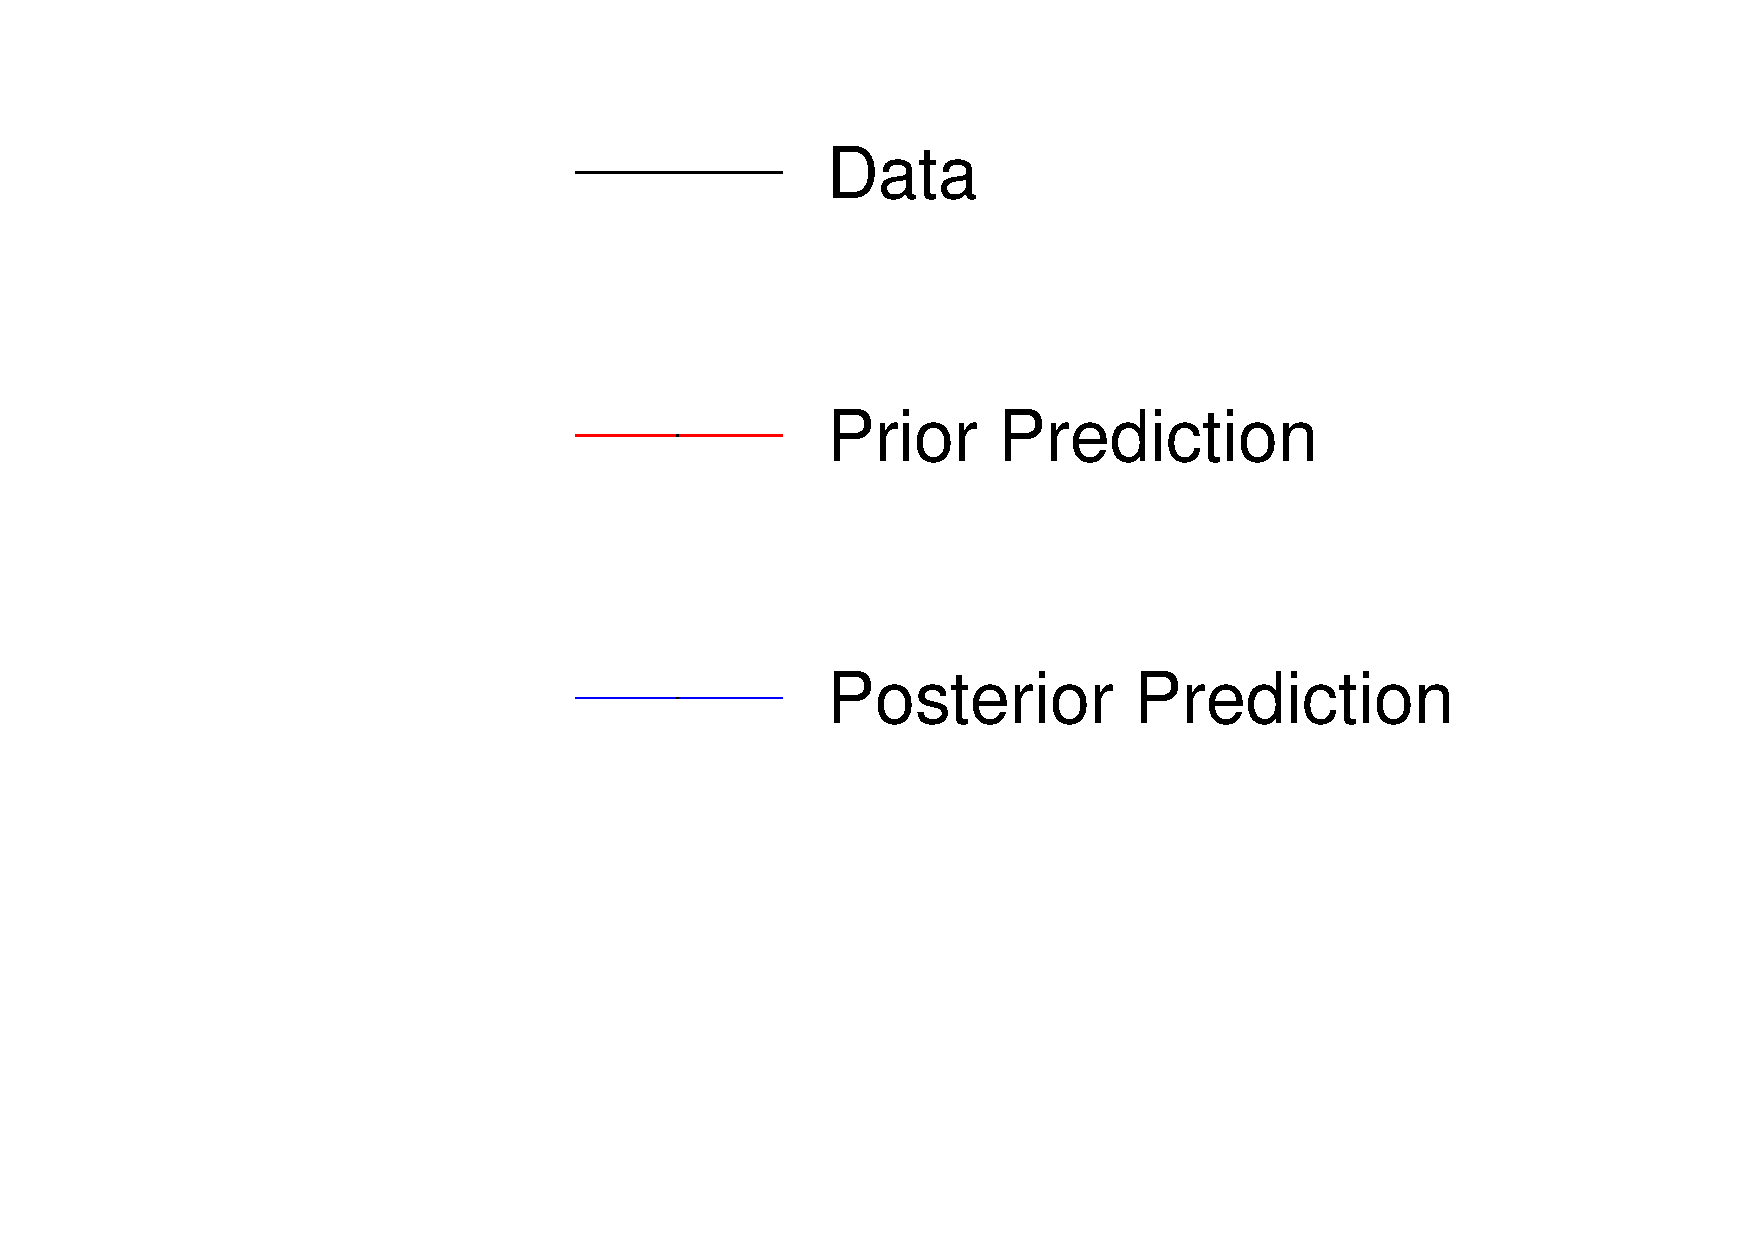
\includegraphics[width=\linewidth, clip]{figs/prior1dleg.pdf}
\end{subfigure}

\begin{subfigure}{0.49\textwidth}
  \centering
  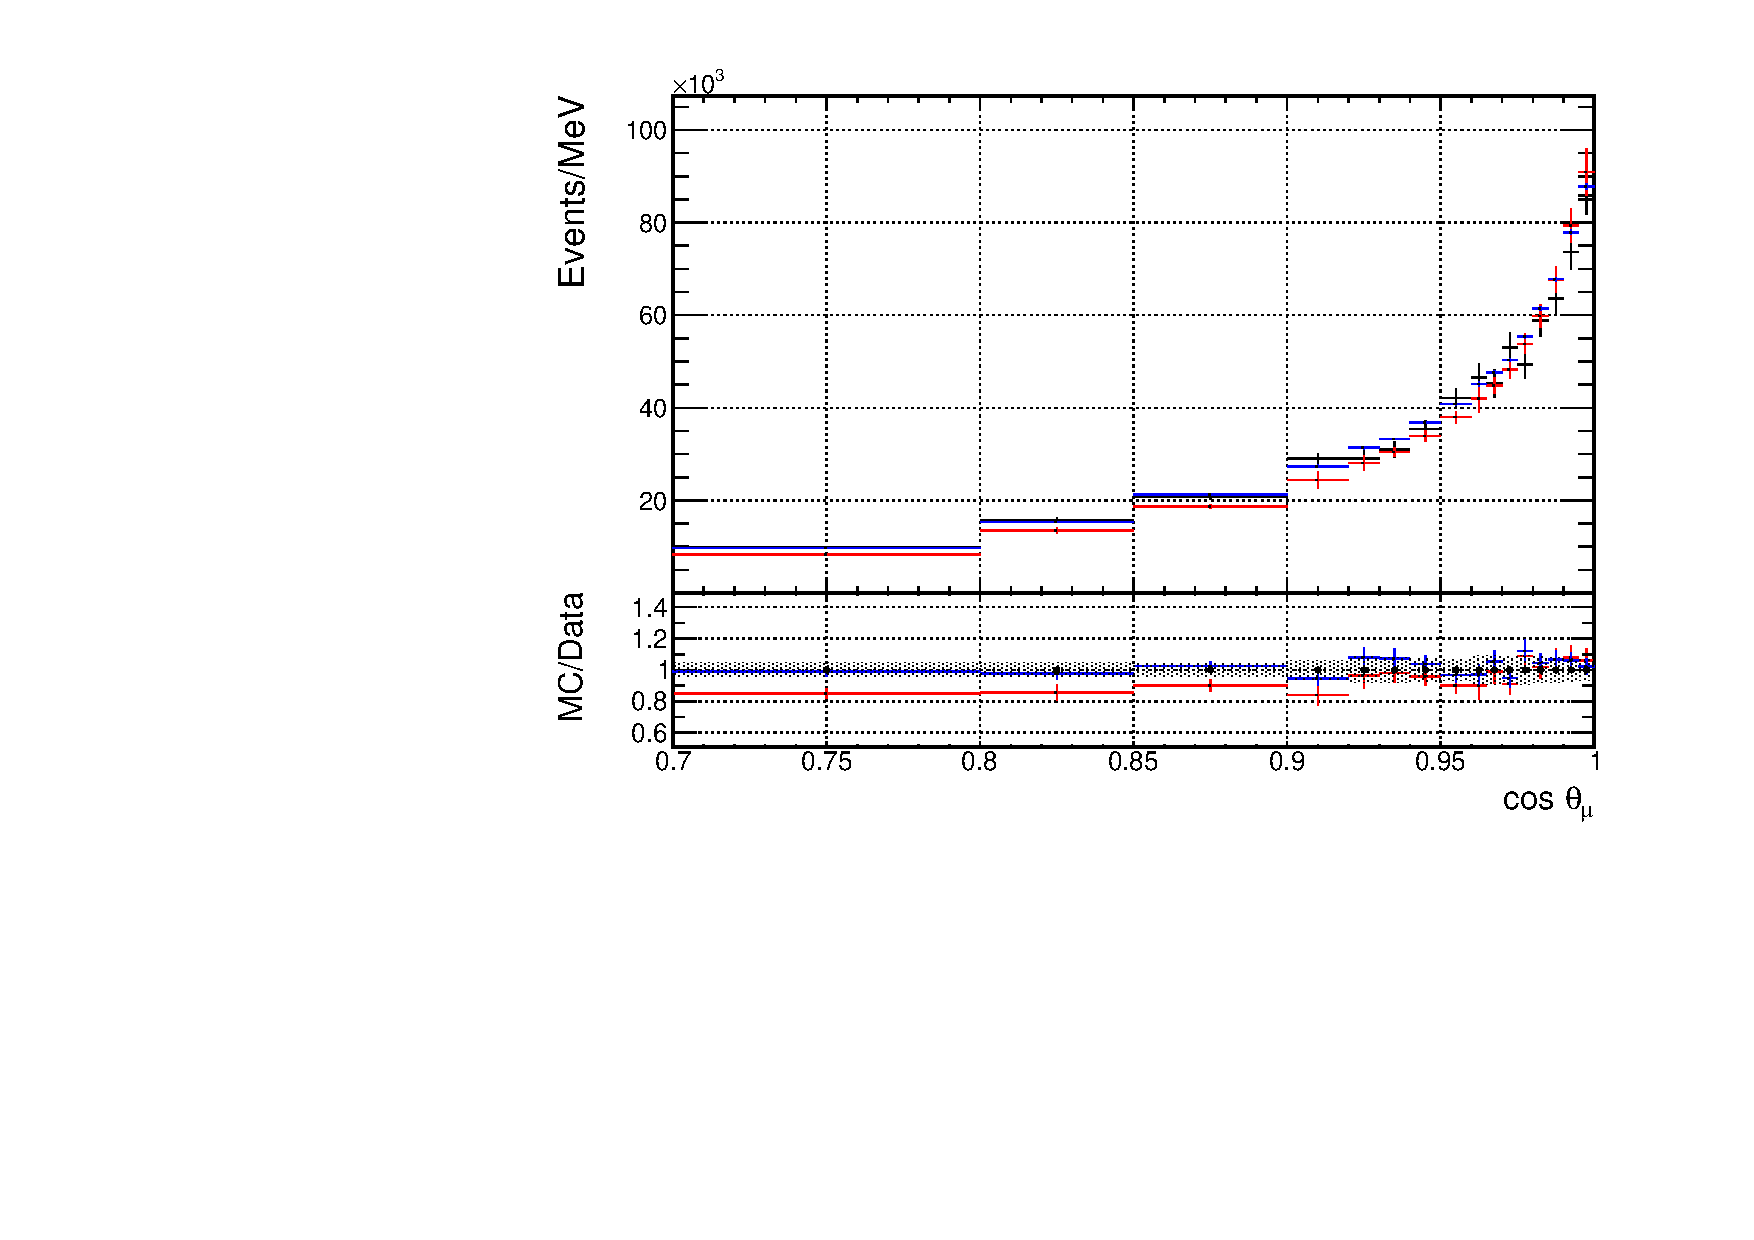
\includegraphics[width=\textwidth]{figs/priorpred1D_t_FGD1_anti-numuCC_0pi}
  \caption{FGD1 RHC $\bar{\nu_{\mu}}$ 0$\pi$}
\end{subfigure}
\begin{subfigure}{0.49\textwidth}
  \centering
  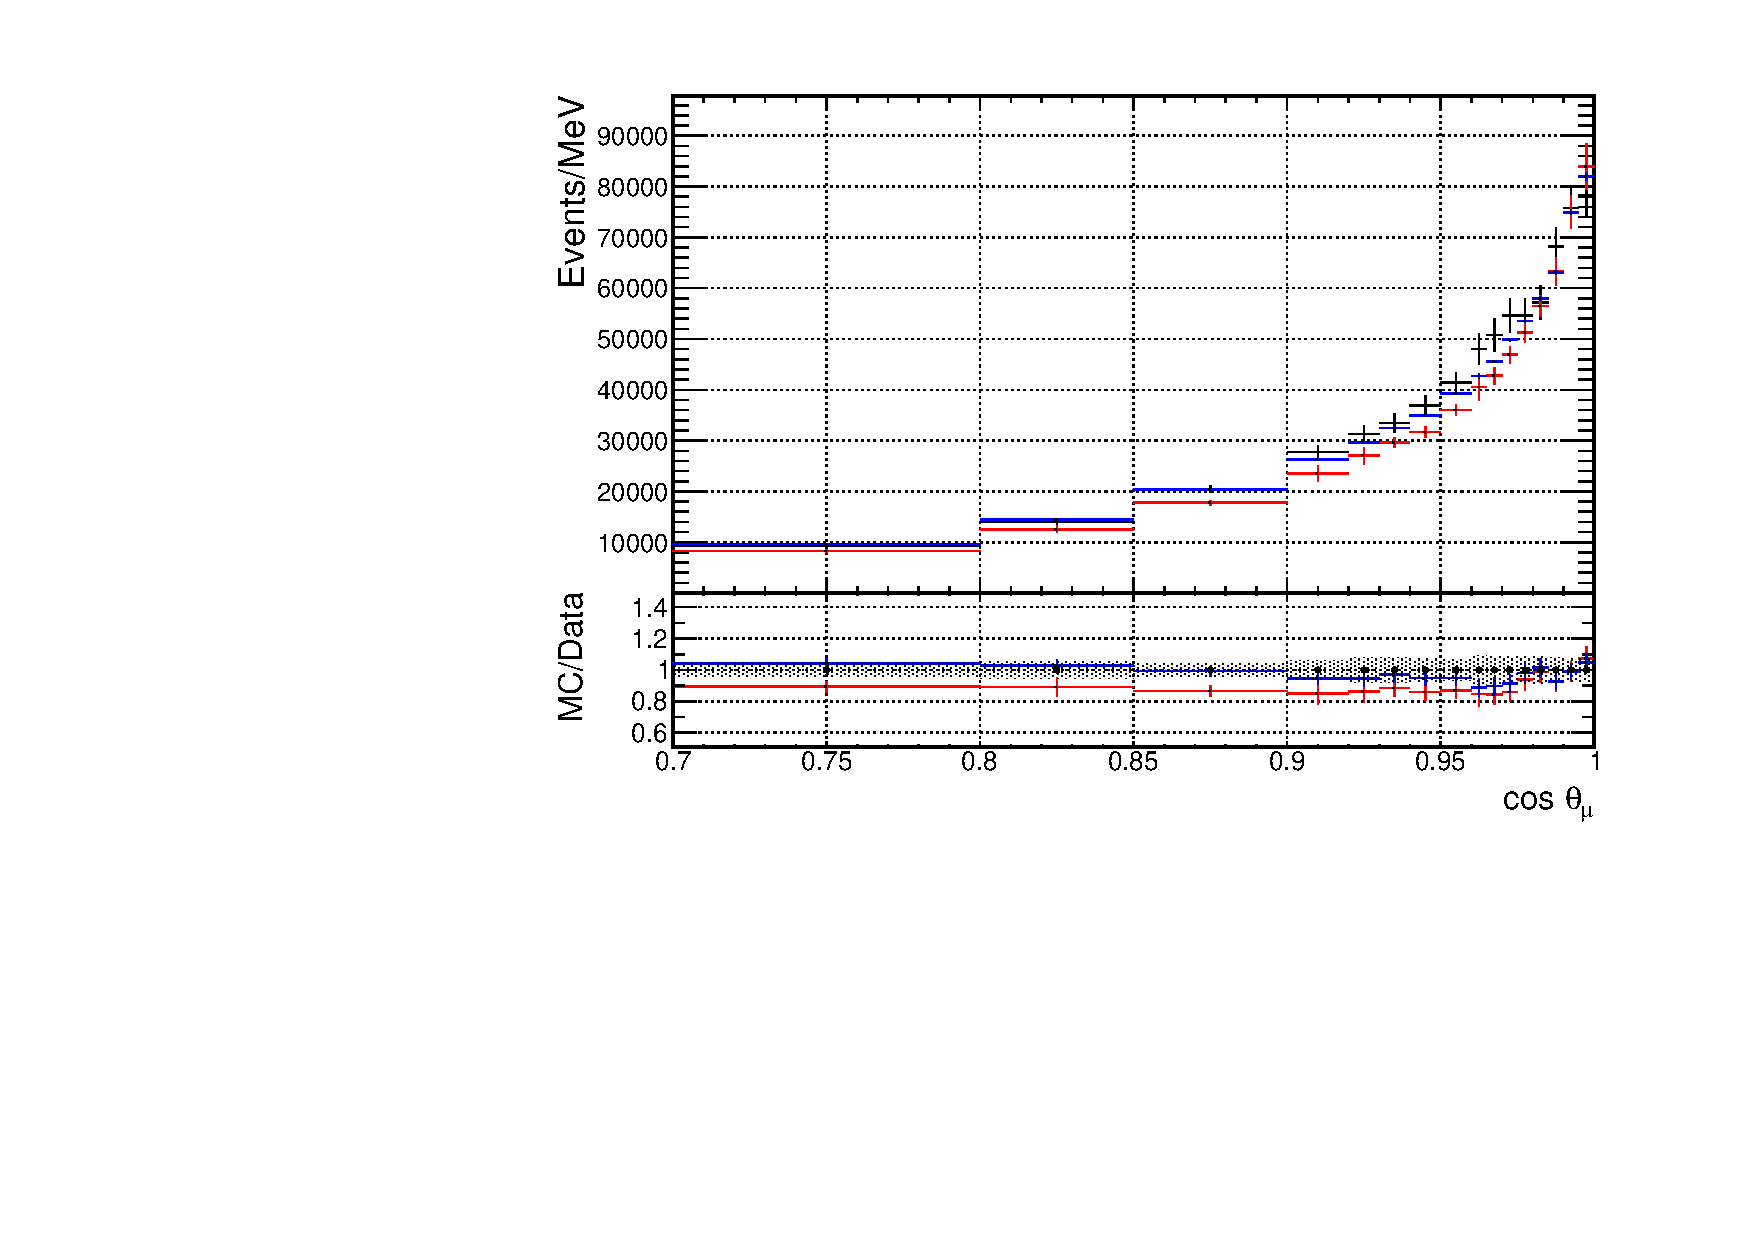
\includegraphics[width=\textwidth]{figs/priorpred1D_t_FGD2_anti-numuCC_0pi}
  \caption{FGD2 RHC $\bar{\nu_{\mu}}$ 0$\pi$}
\end{subfigure}

\begin{subfigure}{0.49\textwidth}
  \centering
  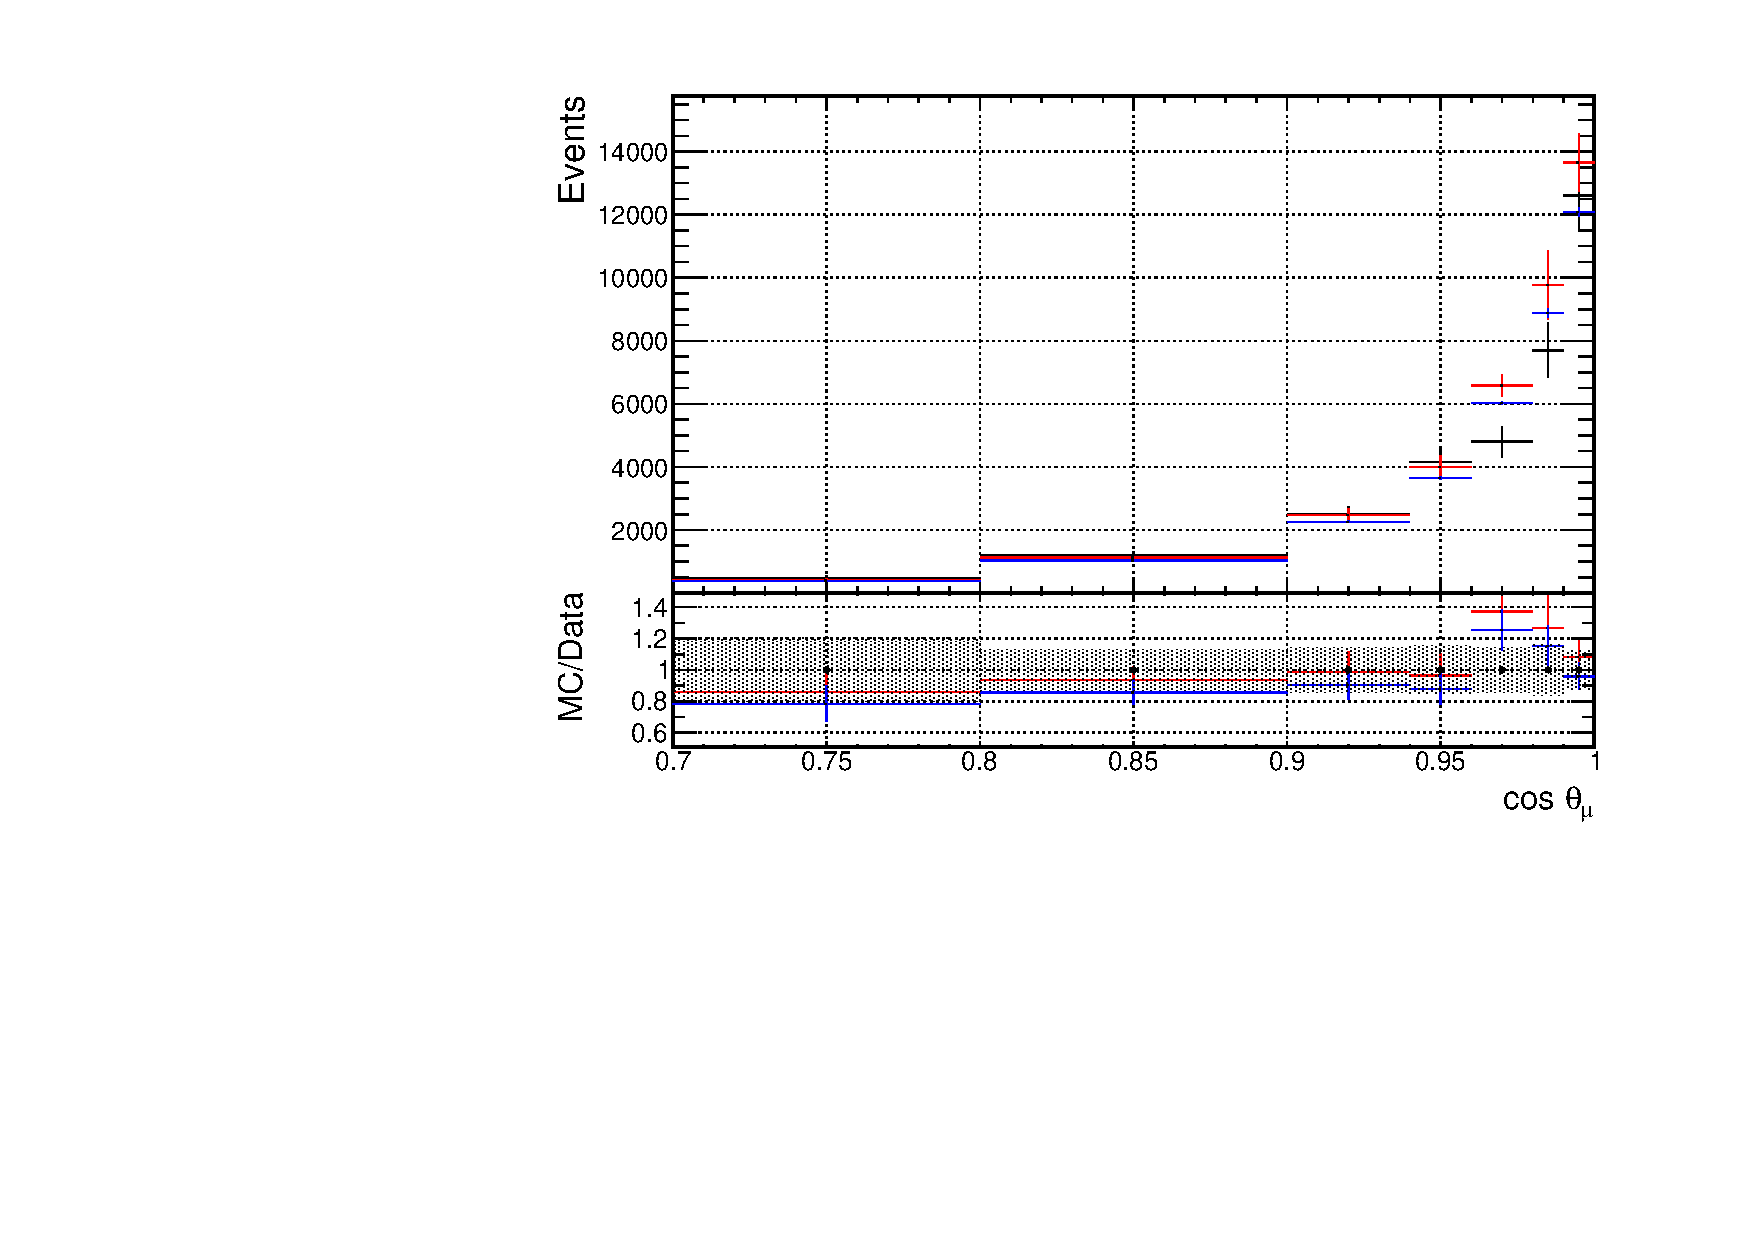
\includegraphics[width=\textwidth]{figs/priorpred1D_t_FGD1_anti-numuCC_1pi}
  \caption{FGD1 RHC $\bar{\nu_{\mu}}$ 1$\pi$}
\end{subfigure}
\centering
\begin{subfigure}{0.49\textwidth}
  \centering
  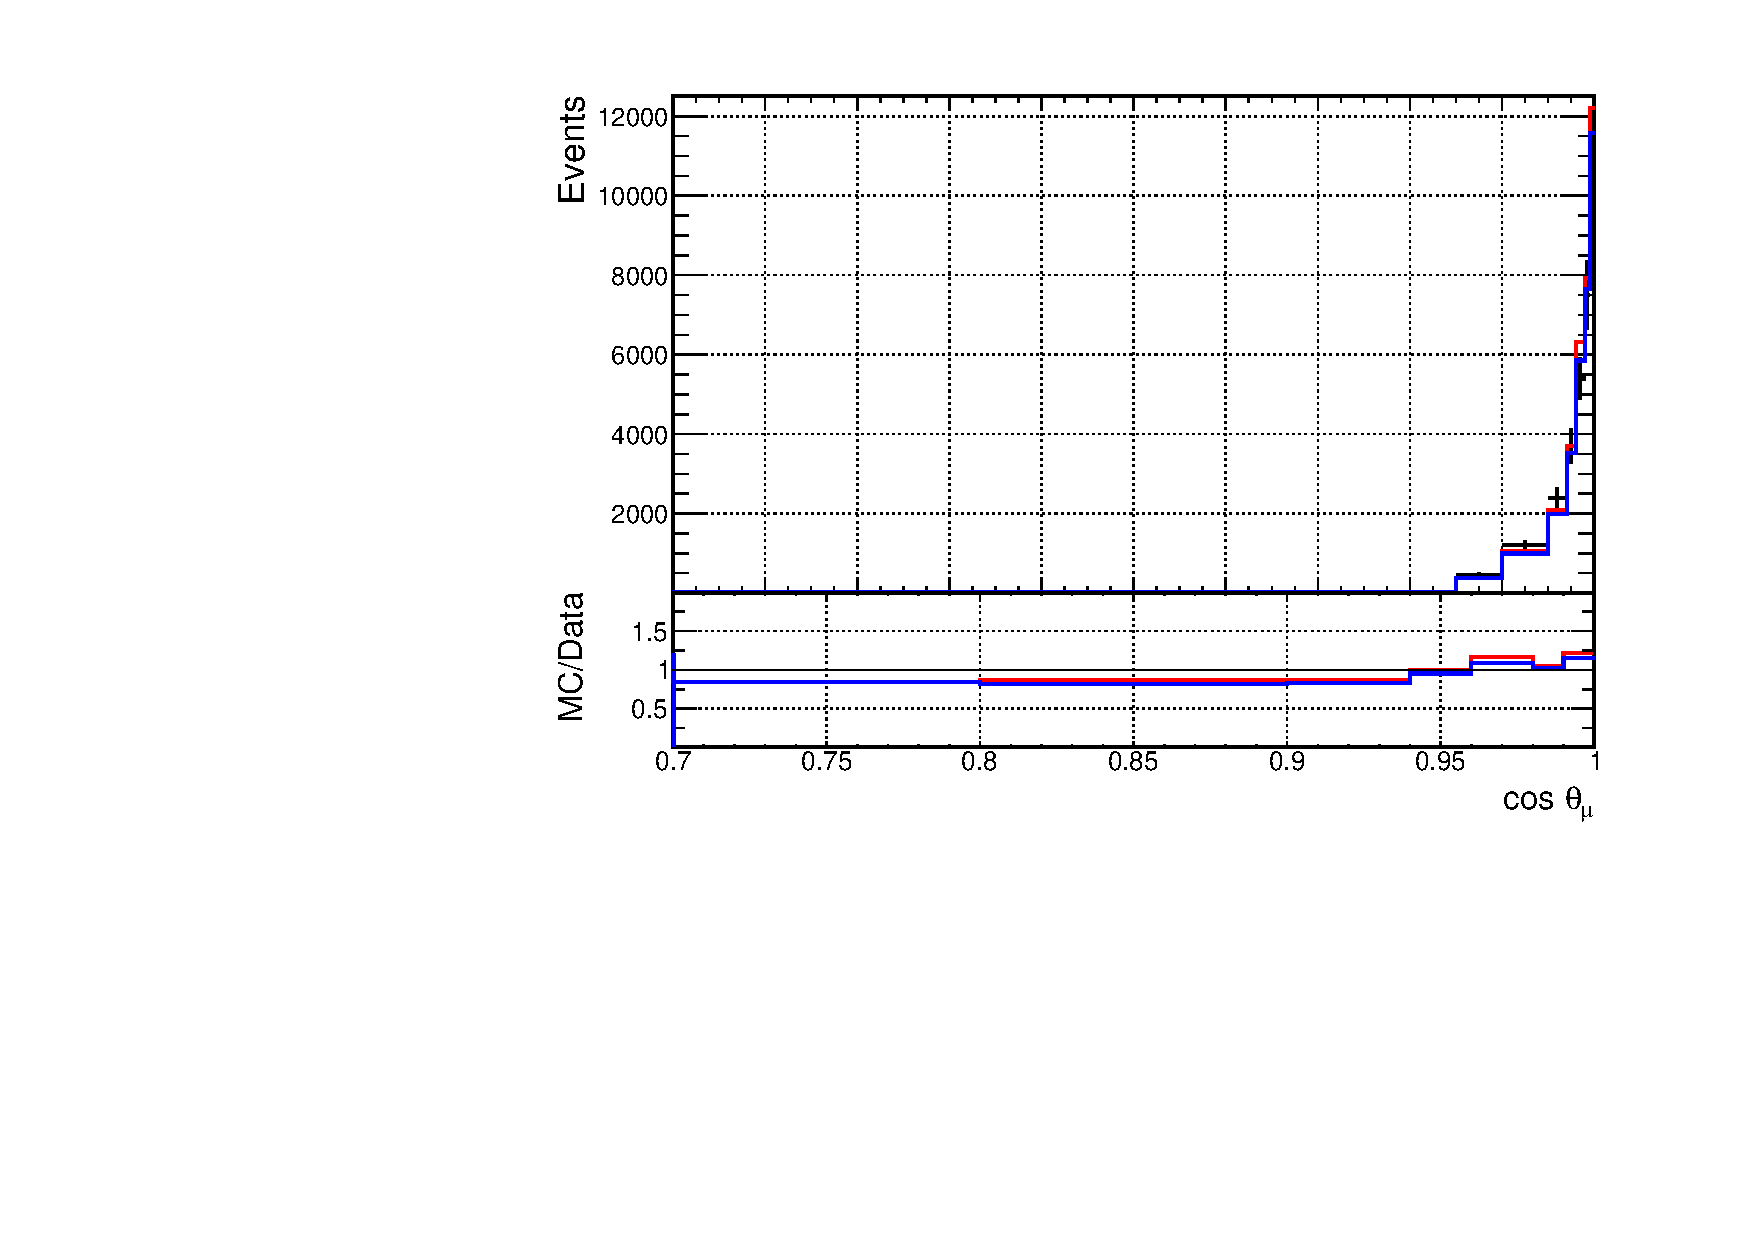
\includegraphics[width=\textwidth]{figs/priorpred1D_t_FGD2_anti-numuCC_1pi}
  \caption{FGD2 RHC $\bar{\nu_{\mu}}$ 1$\pi$}
\end{subfigure}

\begin{subfigure}{0.49\textwidth}
  \centering
  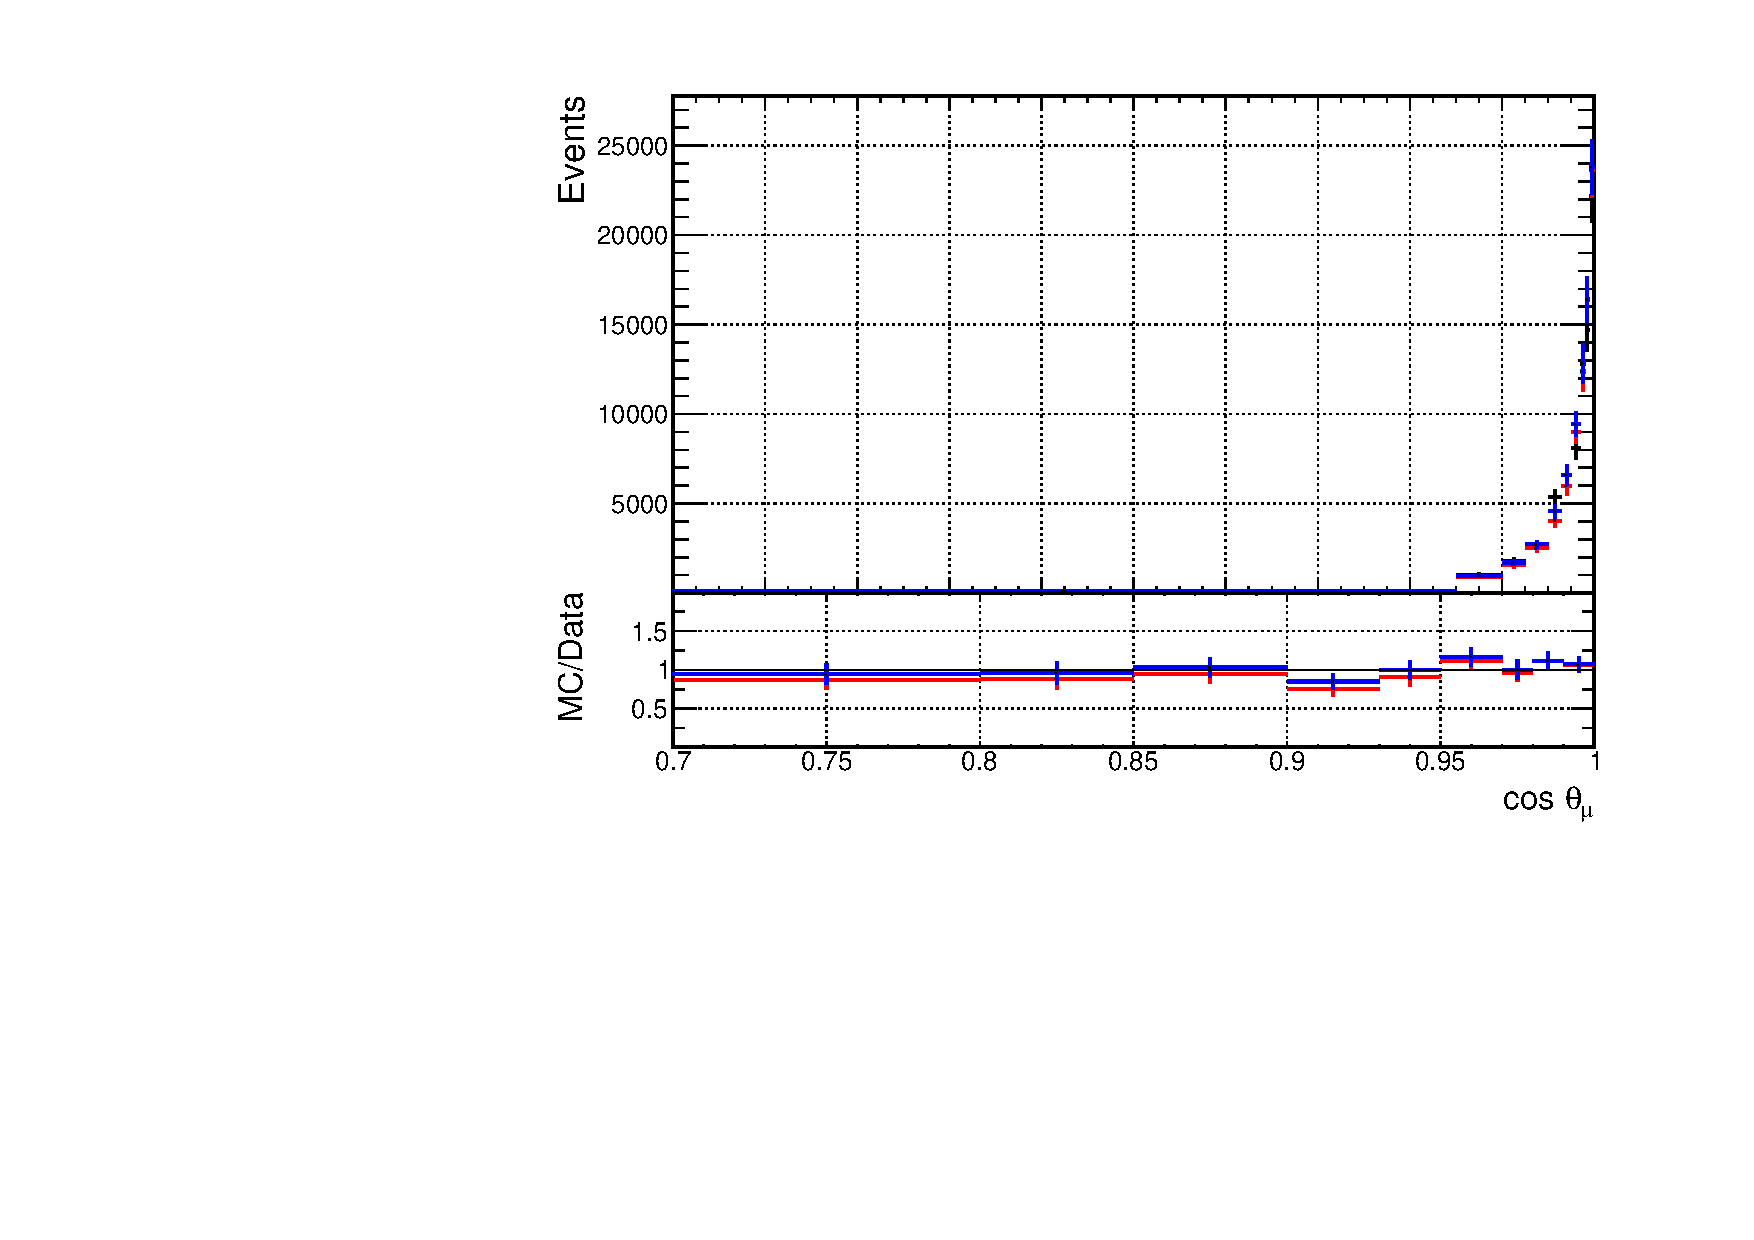
\includegraphics[width=\textwidth]{figs/priorpred1D_t_FGD1_anti-numuCC_other}
  \caption{FGD1 RHC $\bar{\nu_{\mu}}$ Other}
\end{subfigure}
\begin{subfigure}{0.49\textwidth}
  \centering
  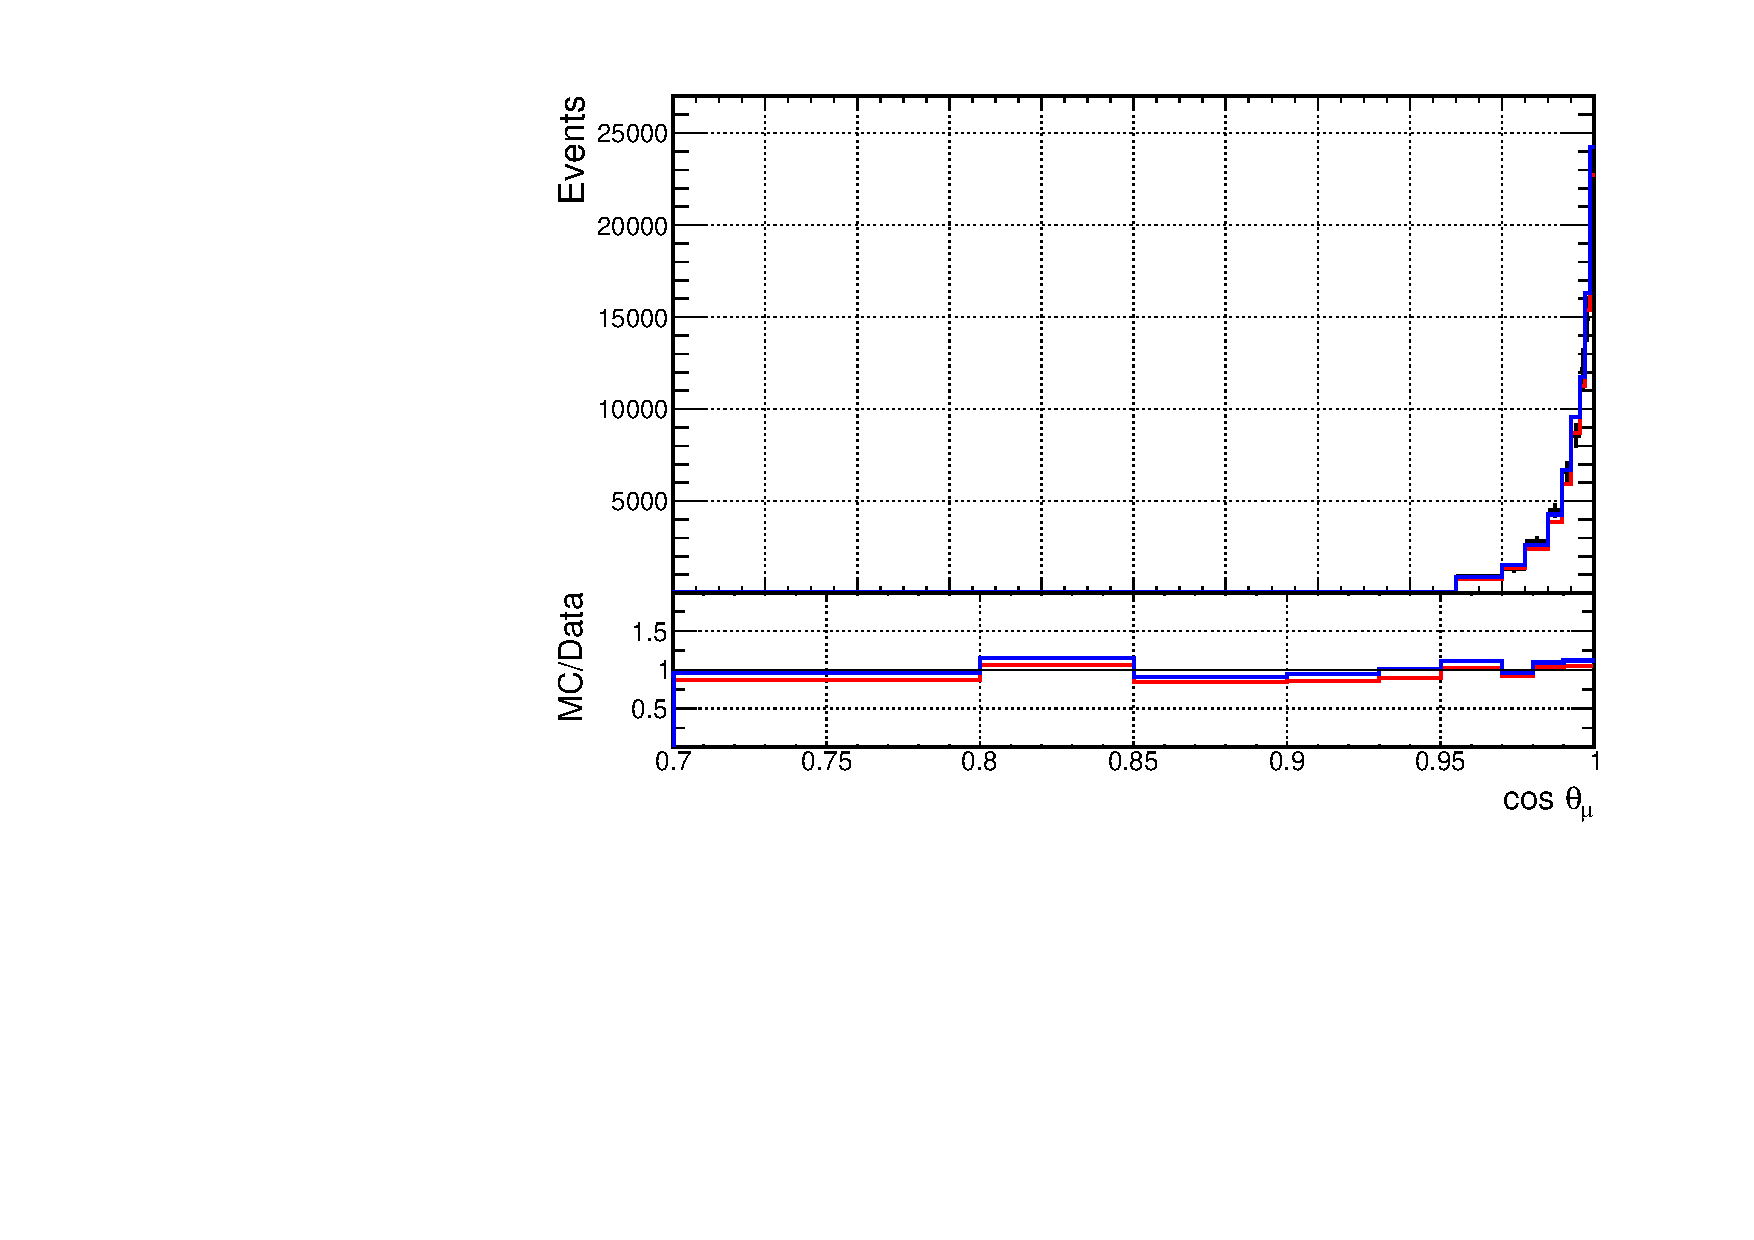
\includegraphics[width=\textwidth]{figs/priorpred1D_t_FGD2_anti-numuCC_other}
  \caption{FGD2 RHC $\bar{\nu_{\mu}}$ Other}
\end{subfigure}
\caption{cos$\theta_{\mu}$ projections of the prior and posterior predictive distributions and data for RHC \numub selections.}
\label{fig:priorpost_rhc_numub_tapp}
\end{figure}

\begin{figure}[!htbp]
\centering
\begin{subfigure}{.24\textwidth}
  \centering
  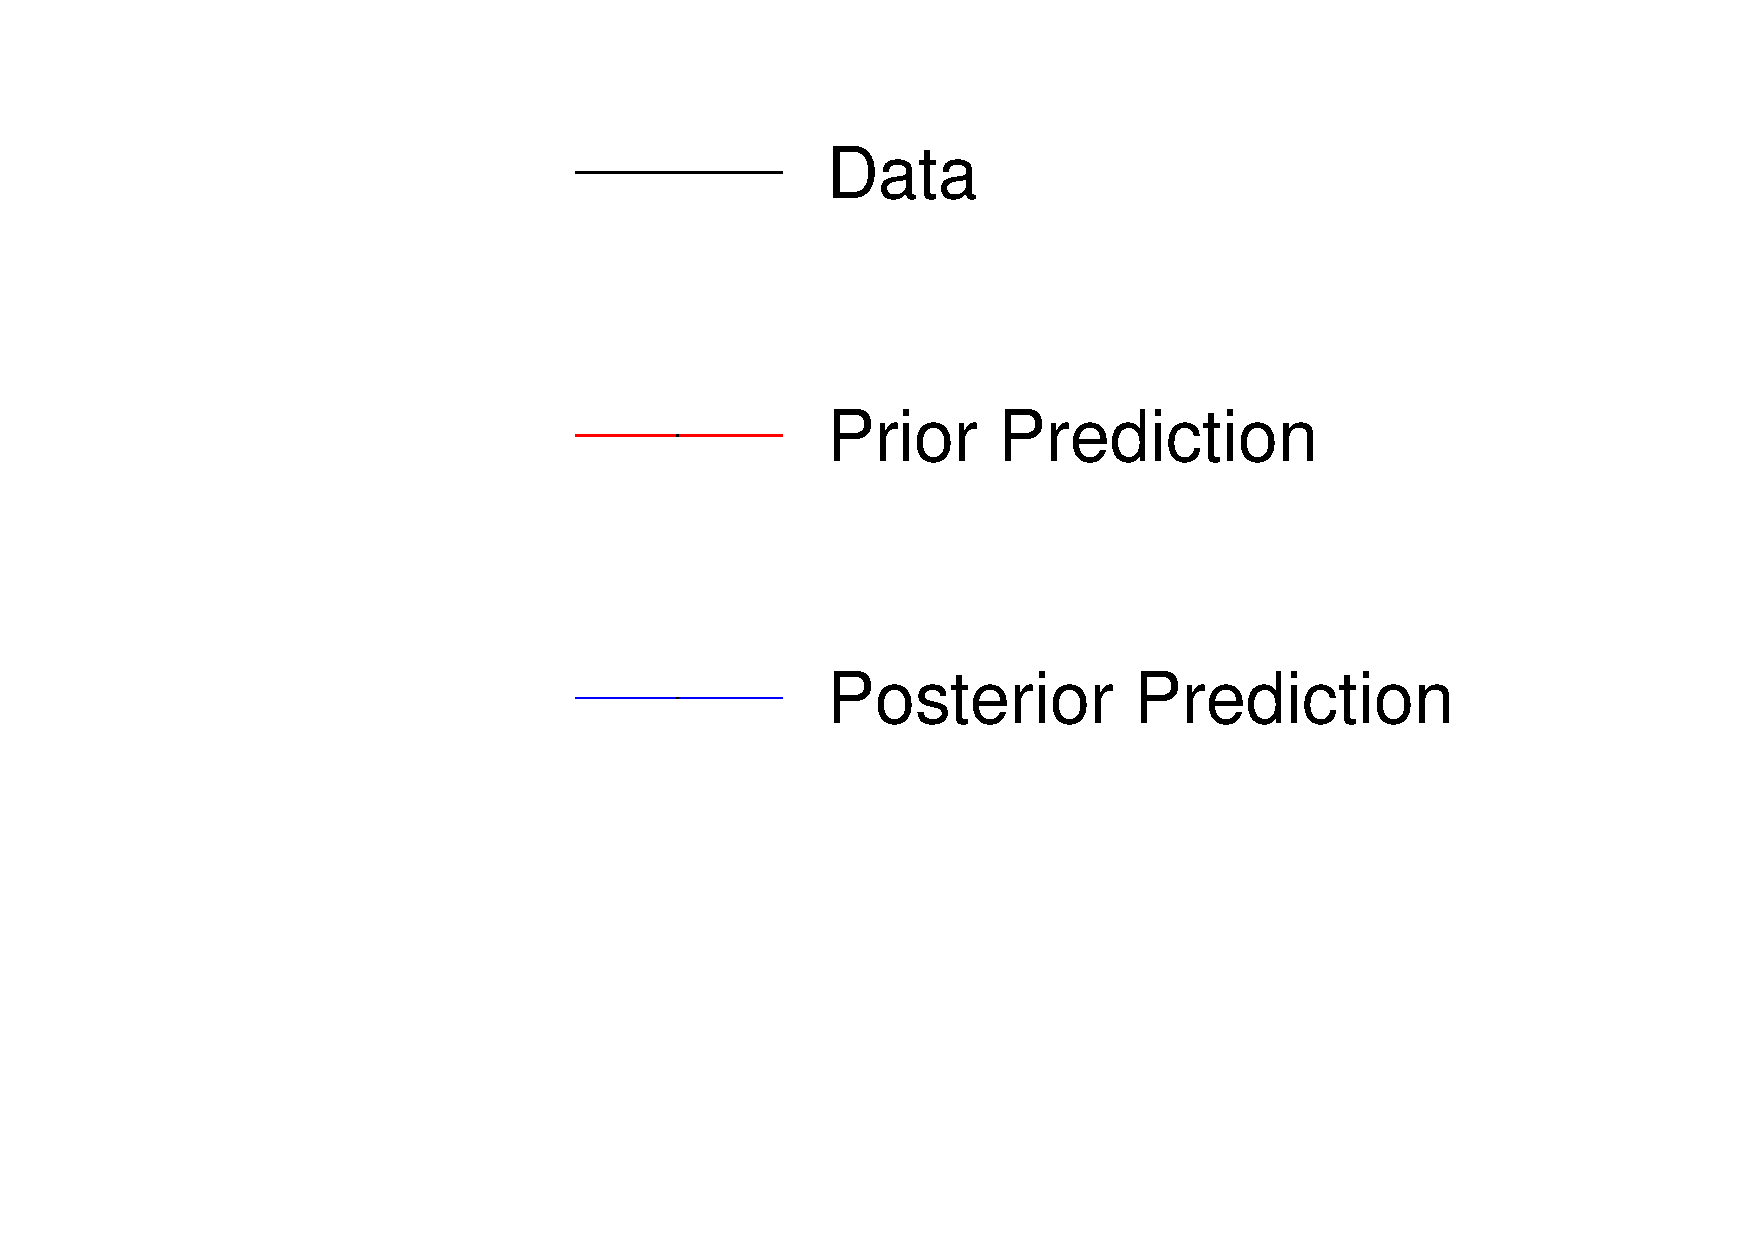
\includegraphics[width=\linewidth, clip]{figs/prior1dleg.pdf}
\end{subfigure}

\begin{subfigure}{0.49\textwidth}
  \centering
  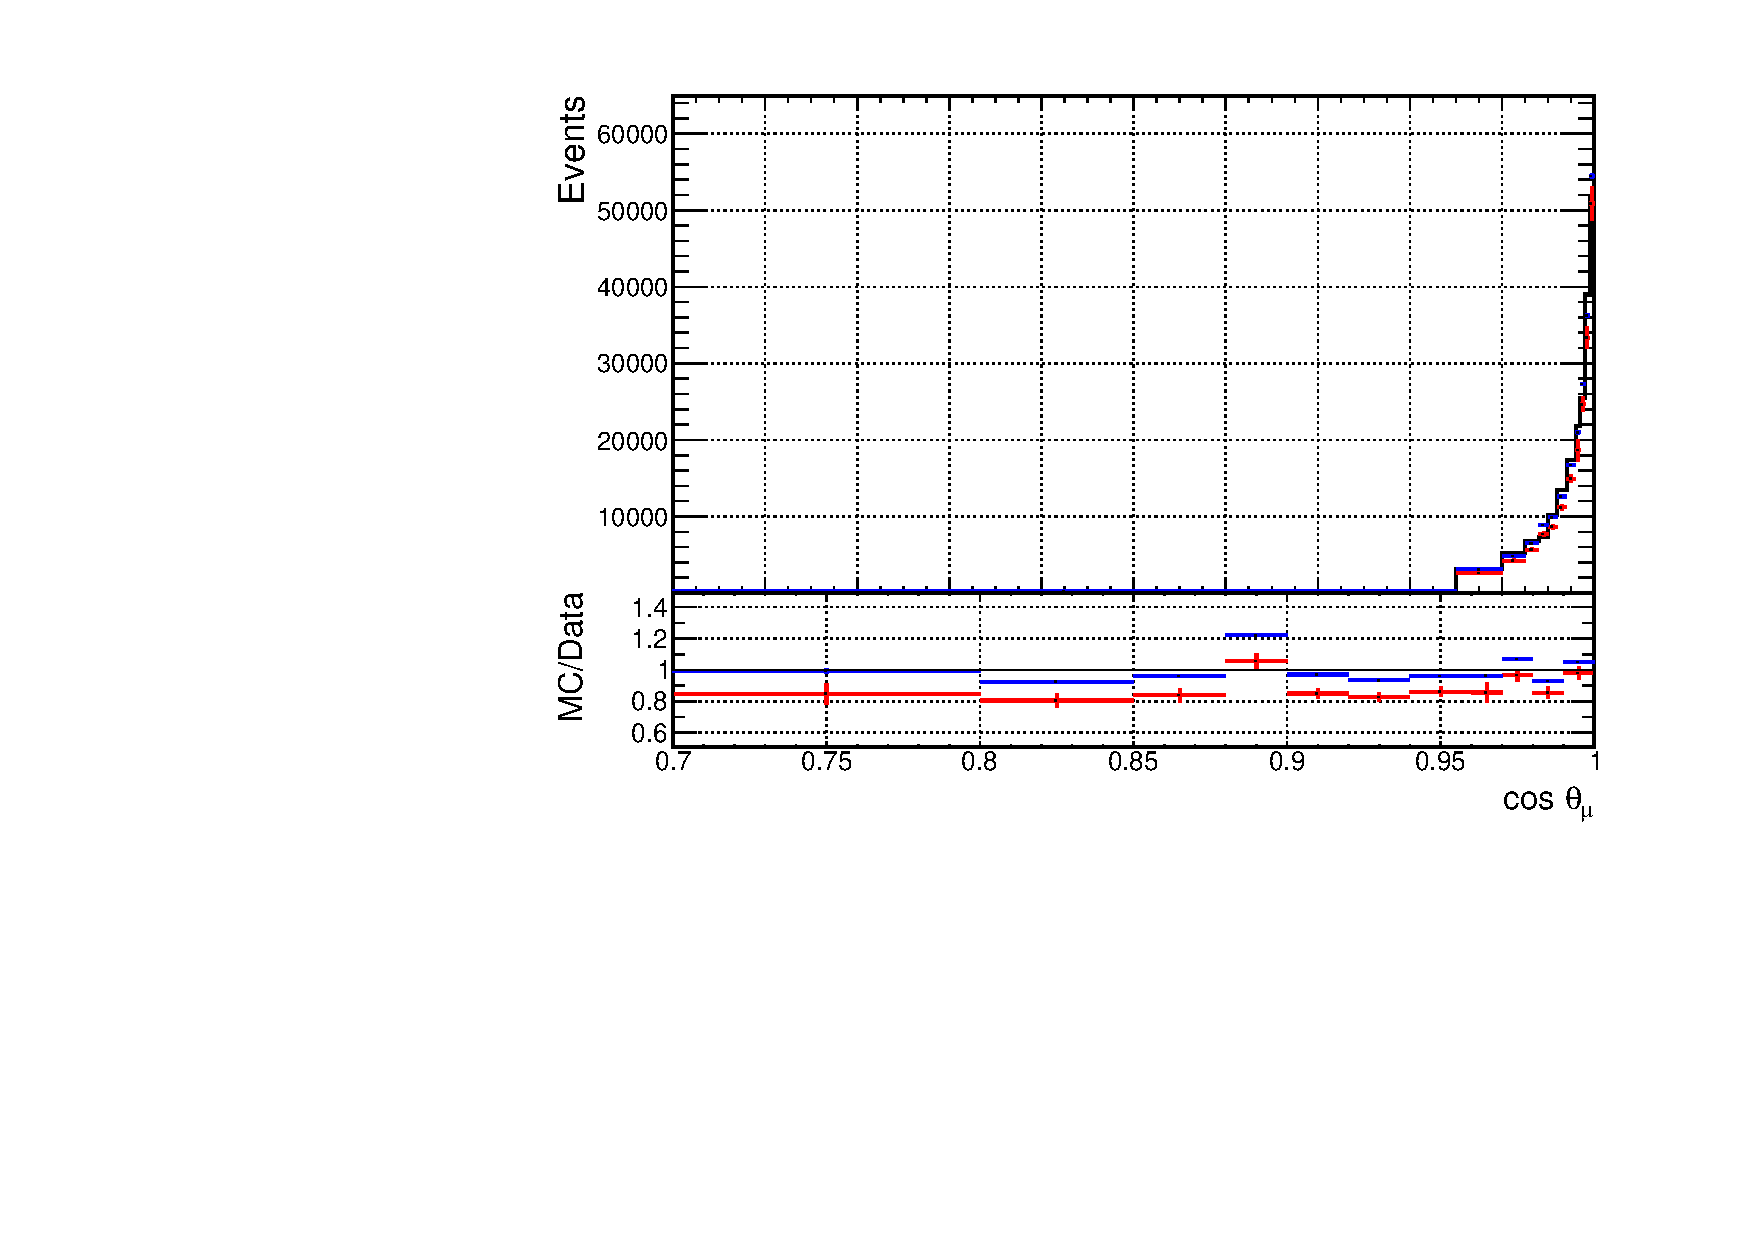
\includegraphics[width=\textwidth]{figs/priorpred1D_t_FGD1_NuMuBkg_CC0pi_in_AntiNu_Mode}
  \caption{FGD1 RHC $\nu_{\mu}$ 0$\pi$}
\end{subfigure}
\begin{subfigure}{0.49\textwidth}
  \centering
  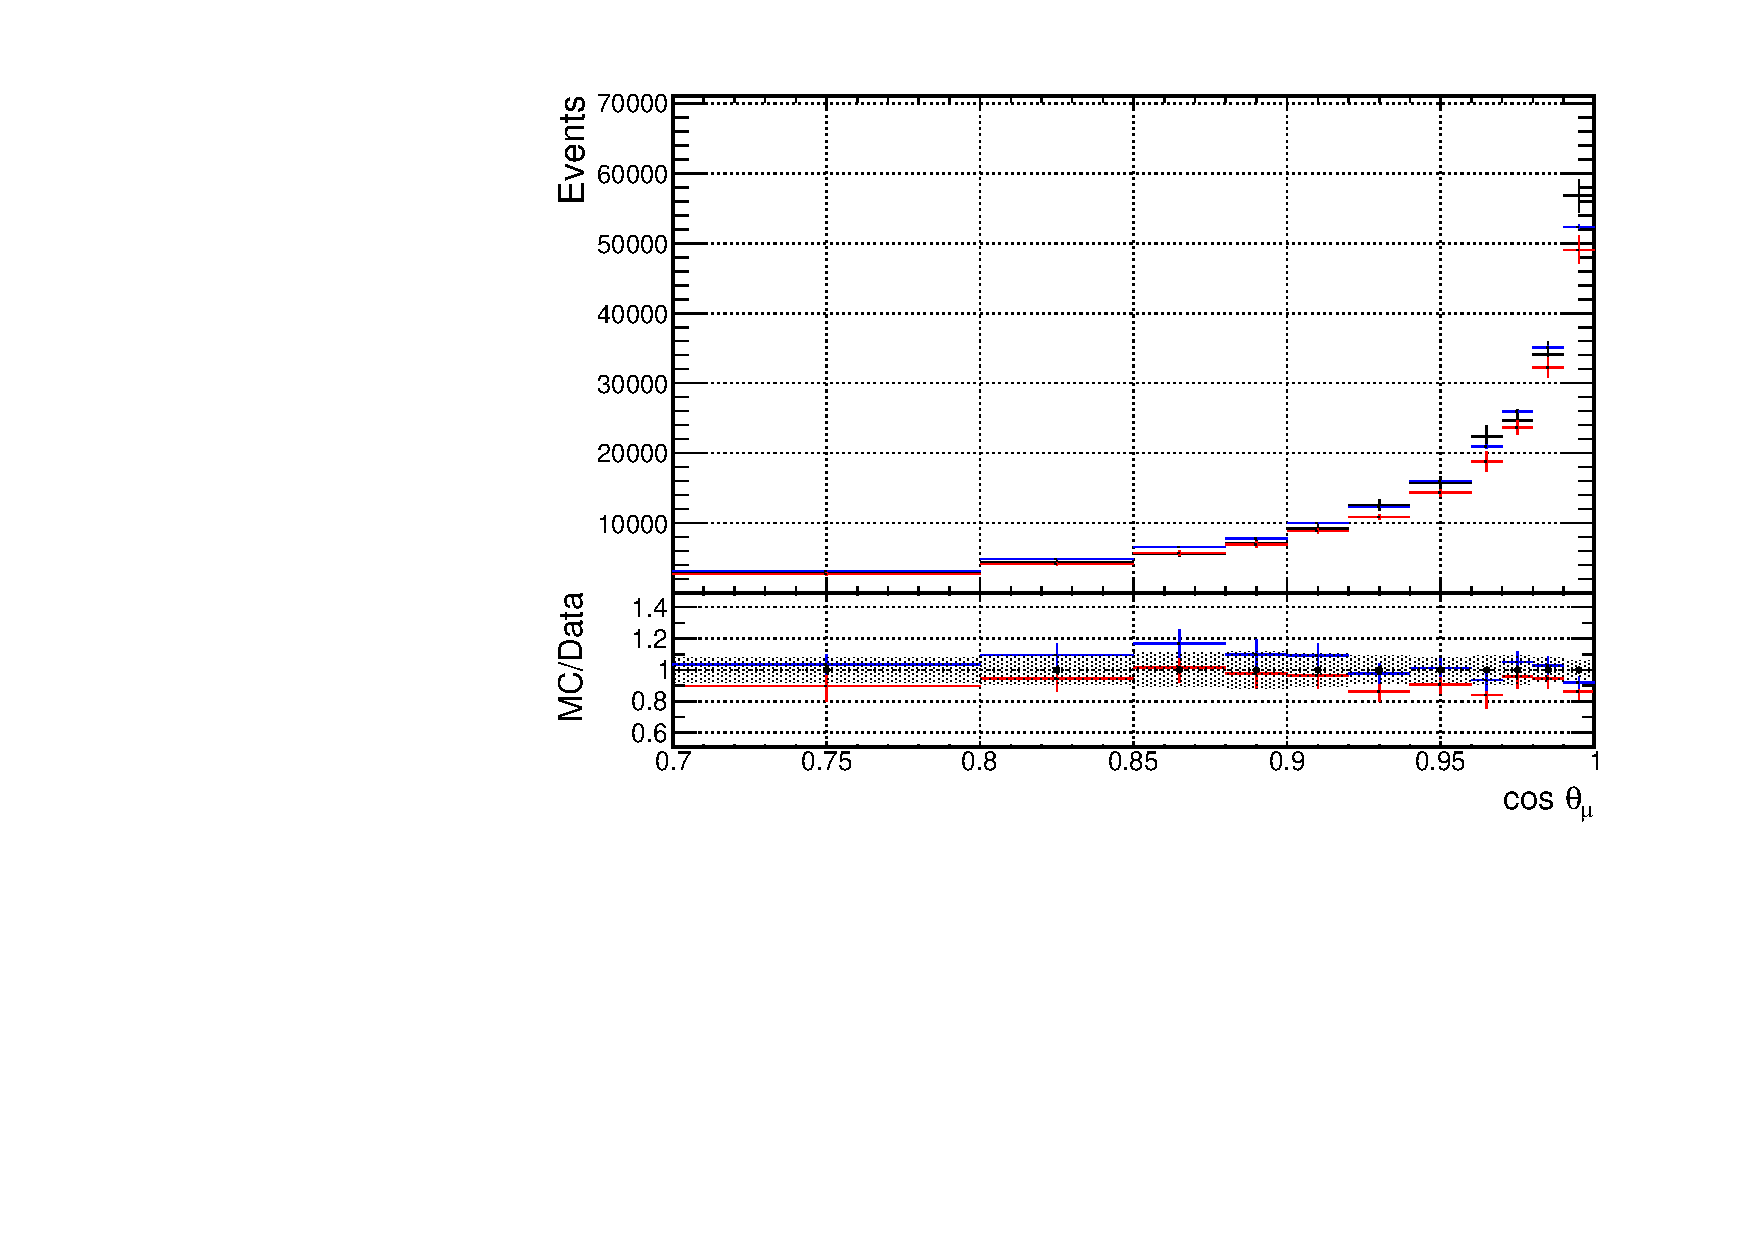
\includegraphics[width=\textwidth]{figs/priorpred1D_t_FGD2_NuMuBkg_CC0pi_in_AntiNu_Mode}
  \caption{FGD2 RHC $\nu_{\mu}$ 0$\pi$}
\end{subfigure}

\begin{subfigure}{0.49\textwidth}
  \centering
  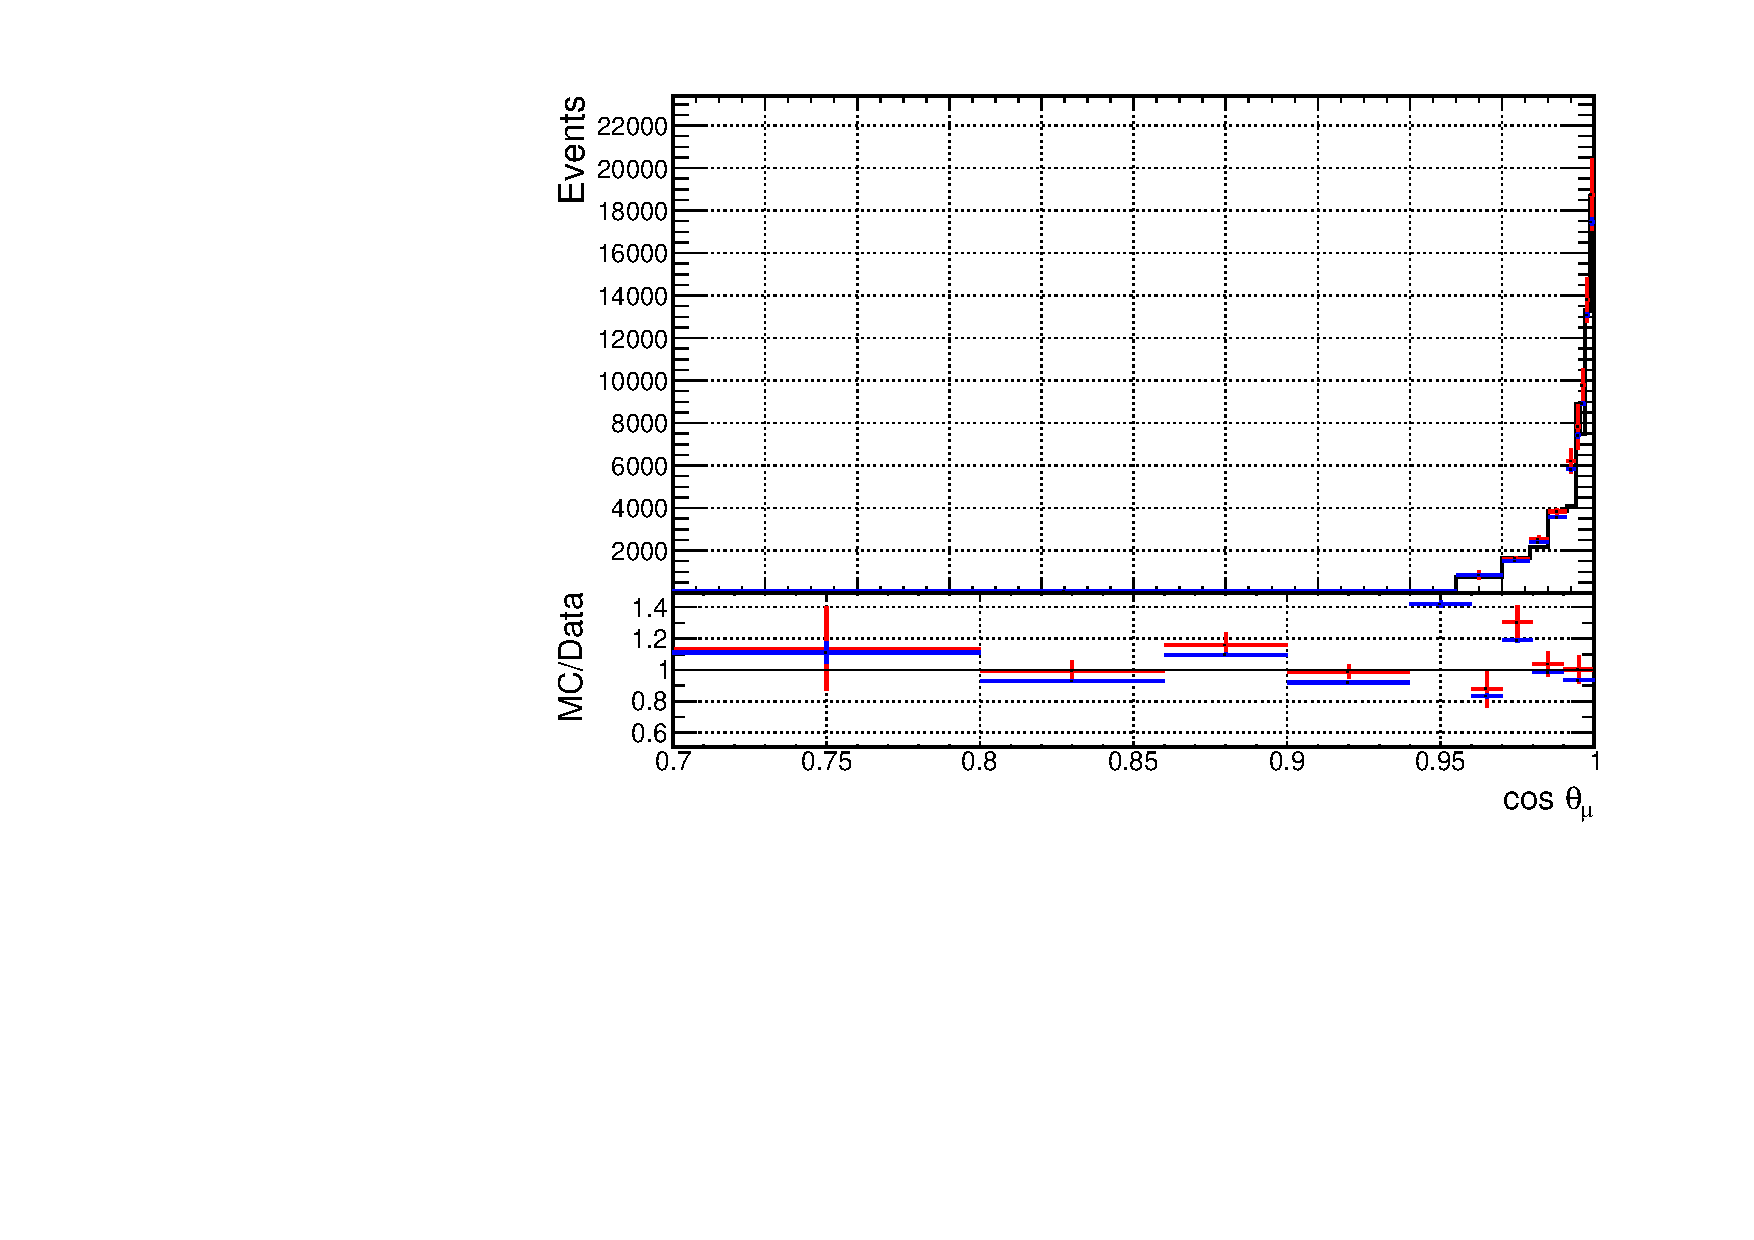
\includegraphics[width=\textwidth]{figs/priorpred1D_t_FGD1_NuMuBkg_CC1pi_in_AntiNu_Mode}
  \caption{FGD1 RHC $\nu_{\mu}$ 1$\pi$}
\end{subfigure}
\begin{subfigure}{0.49\textwidth}
  \centering
  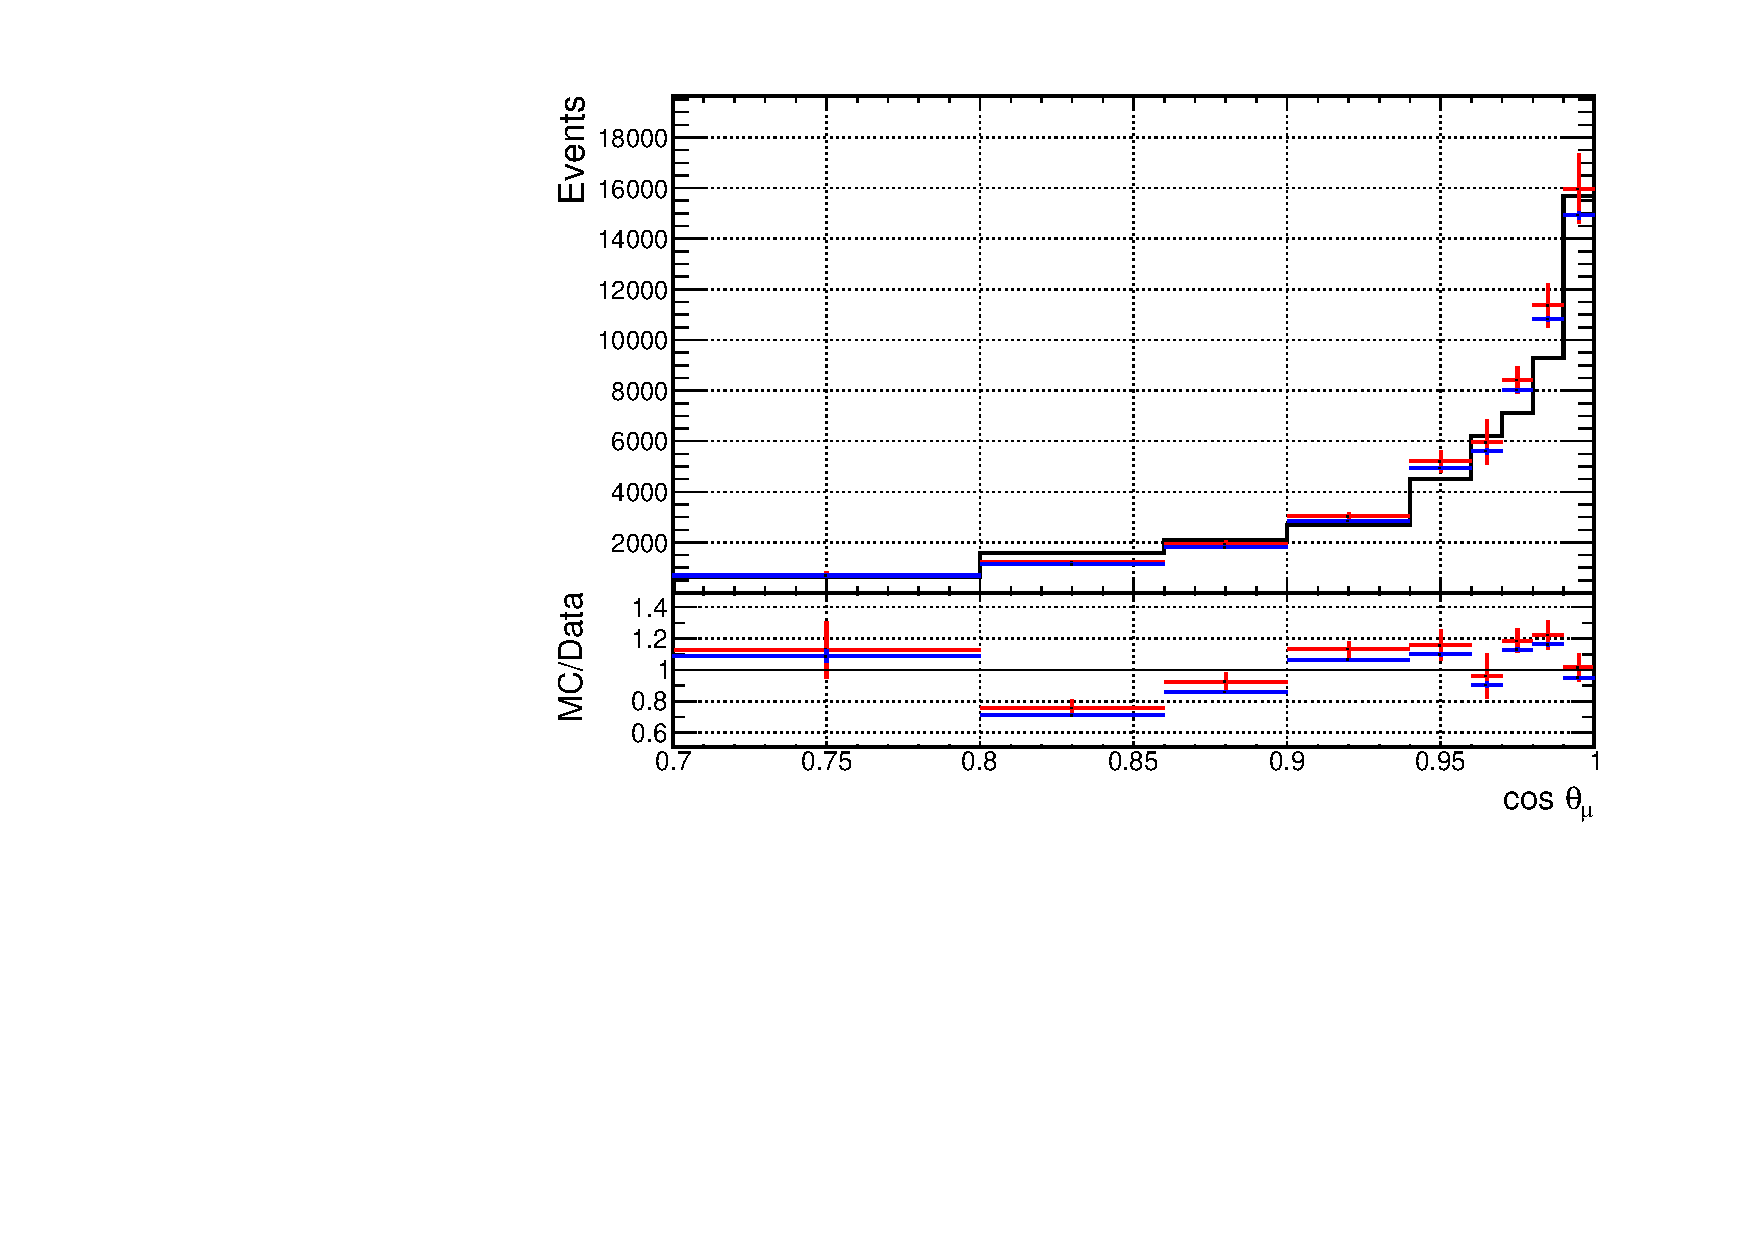
\includegraphics[width=\textwidth]{figs/priorpred1D_t_FGD2_NuMuBkg_CC1pi_in_AntiNu_Mode}
  \caption{FGD2 RHC $\nu_{\mu}$ 1$\pi$}
\end{subfigure}

\begin{subfigure}{0.49\textwidth}
  \centering
  \includegraphics[width=\textwidth]{figs/priorpred1D_t_FGD1_NuMuBkg_CCOther_in_AntiNu_Mode}
  \caption{FGD1 RHC $\nu_{\mu}$ Other}
\end{subfigure}
\begin{subfigure}{0.49\textwidth}
  \centering
  \includegraphics[width=\textwidth]{figs/priorpred1D_t_FGD2_NuMuBkg_CCOther_in_AntiNu_Mode}
  \caption{FGD2 RHC $\nu_{\mu}$ Other}
\end{subfigure}
\caption{cos$\theta_{\mu}$ projections of the prior and posterior predictive distributions and data for RHC \numu selections.}
\label{fig:priorpost_rhc_numu_tapp}
\end{figure}

\newpage